\documentclass[11pt,a4paper]{article}

\usepackage{fullpage}
\usepackage{hyperref}
\usepackage{graphicx}
\usepackage{amsmath}
\usepackage{xcolor}

\usepackage{pdflscape}
\usepackage{afterpage}

\usepackage{footmisc}
\usepackage{caption}

\newcommand{\source}[1]{\vspace{-1em}\caption*{\tiny{Source: \texttt{ {#1} }}} }

\definecolor{red}{RGB}{250, 0, 0}

\usepackage{minted}
% \usemintedstyle{monokai}
\setminted{
    linenos,
    mathescape,
    autogobble,
    showspaces=false,
    fontsize=\small,
    baselinestretch=1
}
\BeforeBeginEnvironment{minted}{\vspace{-0.5em}}
\AfterEndEnvironment{minted}{\vspace{-0.5em}}

\usepackage{everypage}
\usepackage{environ}
\newcounter{abspage}% \thepage not reliab

\makeatletter
\newcommand{\newSFPage}[1]% #1 = \theabspage
  {\global\expandafter\let\csname SFPage@#1\endcsname\null}

\NewEnviron{SidewaysFigure}{\begin{figure}[p]
\protected@write\@auxout{\let\theabspage=\relax}% delays expansion until shipout
  {\string\newSFPage{\theabspage}}%
\ifdim\textwidth=\textheight
  \rotatebox{90}{\parbox[c][\textwidth][c]{\linewidth}{\BODY}}%
\else
  \rotatebox{90}{\parbox[c][\textwidth][c]{\textheight}{\BODY}}%
\fi
\end{figure}}

\AddEverypageHook{% check if sideways figure on this page
  \ifdim\textwidth=\textheight
    \stepcounter{abspage}% already in landscape
  \else
    \@ifundefined{SFPage@\theabspage}{}{\global\pdfpageattr{/Rotate 0}}%
    \stepcounter{abspage}%
    \@ifundefined{SFPage@\theabspage}{}{\global\pdfpageattr{/Rotate 90}}%
  \fi}
\makeatother

\usepackage{fancyhdr}
\pagestyle{fancy}
\fancyhf{}

\renewcommand{\headrulewidth}{0pt}
\renewcommand{\footrulewidth}{0pt}

\fancypagestyle{firstpagefooter} {
    \lfoot{\tiny{Version: 30.11.2017}}
    \cfoot{}
    \rfoot{\thepage}

}

\lfoot{Name: Jakob Beckmann Legi: 17-945-866}
\rfoot{\thepage}

\setlength{\parskip}{0.5em}

\begin{document}

\title{Advanced Systems Lab Report\\ \normalsize{Autumn Semester 2017}}
\author{Name: Jakob Beckmann\\Legi: 17-945-866}
\date{
    \vspace{4cm}
    \textbf{Grading} \\
    \vspace{0.5cm}
    \begin{tabular}{|c|c|}
        \hline  \textbf{Section} & \textbf{Points} \\
        \hline  1                &                 \\
        \hline  2                &                 \\
        \hline  3                &                 \\
        \hline  4                &                 \\
        \hline  5                &                 \\
        \hline  6                &                 \\
        \hline  7                &                 \\
        \hline \hline Total      &                 \\
        \hline
    \end{tabular}
}
\maketitle
\thispagestyle{firstpagefooter}

\newpage

\section{System Overview}
\subsection{Overall Design}
The overall design of the middleware created in this project is quite straight-forward. A single net-thread listens to a server socket and adds any requests sent to this socket to a blocking queue. A fixed number of worker threads then pull requests from the queue and process them one by one. Each of these worker threads is connected to all backend memcached servers at all times. When a request is being processed by a worker thread, this thread calls to at least one memcached server to handle the request. The only exception is an invalid request, such as an unknown command, in which case the middleware does not contact any backend servers.

\begin{figure}[h]
    \centering
    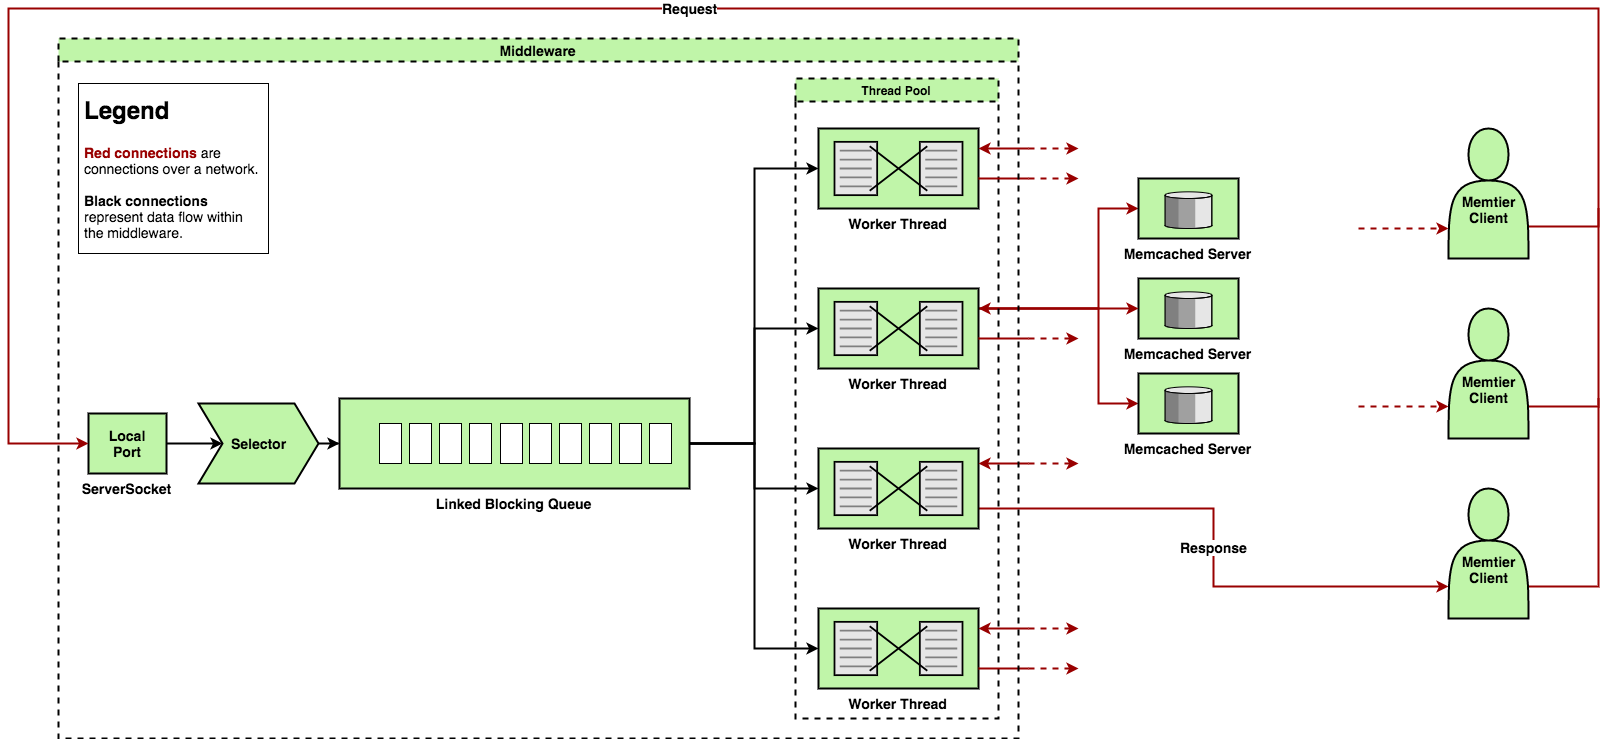
\includegraphics[width=\textwidth]{processing/graphics/system_overview.png}
    \caption{System Overview}
    \label{png::system_overview}
\end{figure}

As can be seen in figure \ref{png::system_overview}, a selector is attached to the server socket in order to accept connections from clients. The key attached to the client connection is then passed with the request such that the workers can communicate the response back to the clients. The selector allows client connections to remain open until explicitly closed by the client. Hence the role of the selector is also to allow new connections and to add them to its internal register of client connections. Once in the internal register (the connection is accepted), the client can send a request which will be read by the net-thread and added to the queue with a reference to the client key. The worker threads then get requests off the queue and process them one by one. The workers first parse the request to get the command type. If the command is invalid, an error message is immediately sent back to the client associated with this request. Otherwise, the worker then communicates with the memcached server(s) in order to store or retrieve data. The servers' response(s) are then parsed again to check for errors and statistics, and a response, potentially merged, is sent to the client.

\subsection{Selector}
The selector serves as a register for connected clients. It is used as passing a socket channel in the queue as part of the request forces the connection to be closed at completion of the request. Hence the selector accepts connections from clients and registers all connected clients. The selector then listens to the registered clients for messages sent to the server socket it is connected to and generates ``read events'' for each client sending messages to the socket. Simultaneously, the net-thread repeatedly checks for read events generated by the selector and reads data from the client associated with the event to a buffer. This buffer is then added as a request to the queue. Note that the selector key and a timestamp are added to the buffer to form a complete request on the queue. The use of a selector forces to use non-blocking IO on the client side. However, this is not a problem since any read event guarantees that data can be read from the socket, hence avoiding the use of reading loops.

\subsection{Worker Threads}
A thread pool executor of fixed size is used to organise the worker threads. This has the advantage that it reduces thread environment switching overhead if there is no need for an extra thread to be used. This could be the case when the connection to the memcached servers are extremely fast. In such a case, the executor will not use more threads than are available from the hardware as reusing the same thread to process the next request does not involve any overhead compared to switching to another thread to perform the same work. However, as soon as server service times increase, the thread pool allows to perform work on some thread while another is idle awaiting a response from memcached. Moreover, the thread pool executor has the advantage that if some thread crashed during the execution of the middleware, it will automatically be relaunched. Hence it should in theory provide more stability to the system.

The worker threads perform close to the entirety of the work within the middleware. The reason these threads perform the most work is that the work can be performed concurrently and, ideally, it is performed in parallel. In the initial design, even the reading from the socket was performed by the workers to avoid creating a buffer (containing the message sent from the client) for each request. However, this leads to request duplication as the read event is active as long as nothing is read from the socket, hence repeatedly adding requests to the queue if the initial request had not been read already. This is easily caused by even non-significant queue times. Therefore the design was changed, at the cost of creating a buffer for each request.

When launching a thread, two buffers are created. One is used for temporary data while the other contains the response from memcached to be sent back to clients. Note that all buffers used in the middleware are of size 16384 bytes as this allows for 10 keys of size 250 bytes and 10 values of 1024 bytes (and some margin) to be stored in the buffer. The temporary data buffer is mostly used to interpret individual responses from the memcached servers and its data is then added to the buffer containing the aggregate data for the client. Creating only two buffers for each worker, without adding buffers for the processing of each request, has the goal to reduce dead times created by the garbage collector. Exactly how individual request types are handled by the middleware and how the buffers are utilised is explained in a later section.

Each worker is connected to all backend memcached servers at all times. These channels are blocking to ensure that the worker awaits a response from the servers when reading from a channel. Should a worker crash, the thread pool executor will rebuild a thread to replace it and the connections to the servers should be reestablished. However, note that such a situation never occurred during testing.

\subsection{Requests}
All requests are built from the following:
\begin{itemize}
    \item A buffer containing the data sent from the client. This is known when the request object is created.
    \item A selection key that refers to the client who sent the request. This is used to recover the channel to said client in order to send him the response. Note this has nothing to do with the memcached key used to refer to the data stored on the backend servers.
    \item A type which can be either:
    \begin{enumerate}
        \item GET: a simple get request with a single key.
        \item SET: a simple set request with one key and the data to be set as the value for that key.
        \item MULTIGET: a get request with more than one key.
        \item INVALID: a request that does not conform to the protocol defining the format of the three commands above.
    \end{enumerate}
    This is not known when the request is created and will only be known once a worker parses the request.
    \item A boolean identifying the request as a hit. Note that the notion of hit is different for each type of request. In the case of a \mintinline{java}{get}, it simply identifies whether a value was returned by the memcached servers. In the case of a \mintinline{java}{set}, this represents whether a server responded with something different to \mintinline{java}{STORED}. In the cases of \mintinline{java}{multiget} and \mintinline{java}{invalid} request, this boolean does not have any meaning. \mintinline{java}{multiget} hits are handled directly as the responses from memcached are parsed.
    \item Several timestamps:
    \begin{enumerate}
        \item The time the request is created. This is (obviously) known when the request is created.
        \item The time the request is dequeued. The worker updates this timestamp as soon as the request is taken from the queue.
        \item The time the request was transmitted to the servers. This timestamp is taken just before any messages are sent to memcached.
        \item The time memcached answered. This is taken once \textit{all} memcached servers that were contacted for this request have answered.
        \item The time the request was completed. This is the timestamp taken when the complete response was sent back to the client.
    \end{enumerate}
\end{itemize}

All requests are parsed only at the worker level, hence the majority of the fields defined above are only known once the request is being processed by some worker.

When parsing a request, the first aspect that is checked is whether the request terminates with \mintinline{java}{"\r\n"}. Then the command is parsed up to the first occurrence of \mintinline{java}{"\r\n"}. The set of bytes preceding these two characters is converted to a string and the first word in said string is compared to known command words (i.e. \mintinline{java}{get} or \mintinline{java}{set}). Once it is established which type the command is, the rest of the command is checked for correctness. In the case of \mintinline{java}{get}, the number of arguments is checked in order to determine whether the command should be treated as a \mintinline{java}{multiget}. In the case of a \mintinline{java}{set}, it is checked if the data block attacked to the request is of the length specified in the command. If any of these tests fail, the command is flagged as invalid and an error string is sent back to the client. In this case there is no communication with the backend memcached servers as the request does not conform to the protocol.

\subsubsection{Sets}
Once a command has been dequeued, parsed, and established as type \mintinline{java}{set}, all worker buffers are cleared and the original request buffer is transmitted to all backend servers. The worker thread then awaits responses from the servers in the same order as he sent out the request. As we use blocking input/output on the server side, the same order is chosen as the first contacted server is likely the first to respond. Note however that if the connection to the first memcached server is significantly slower than other connections, this will result in inefficient time utilisation as the middleware will wait for this response first, even though the responses from other servers might already be available. Every response is then checked, and if anything other than \mintinline{java}{"STORED\r\n"} is returned from any server, that response is returned to the client and the \mintinline{java}{set} is flagged as a miss. The rest of the servers' responses are read in order to make sure all communication channels are cleared for the next request.
\begin{figure}[h]
    \centering
    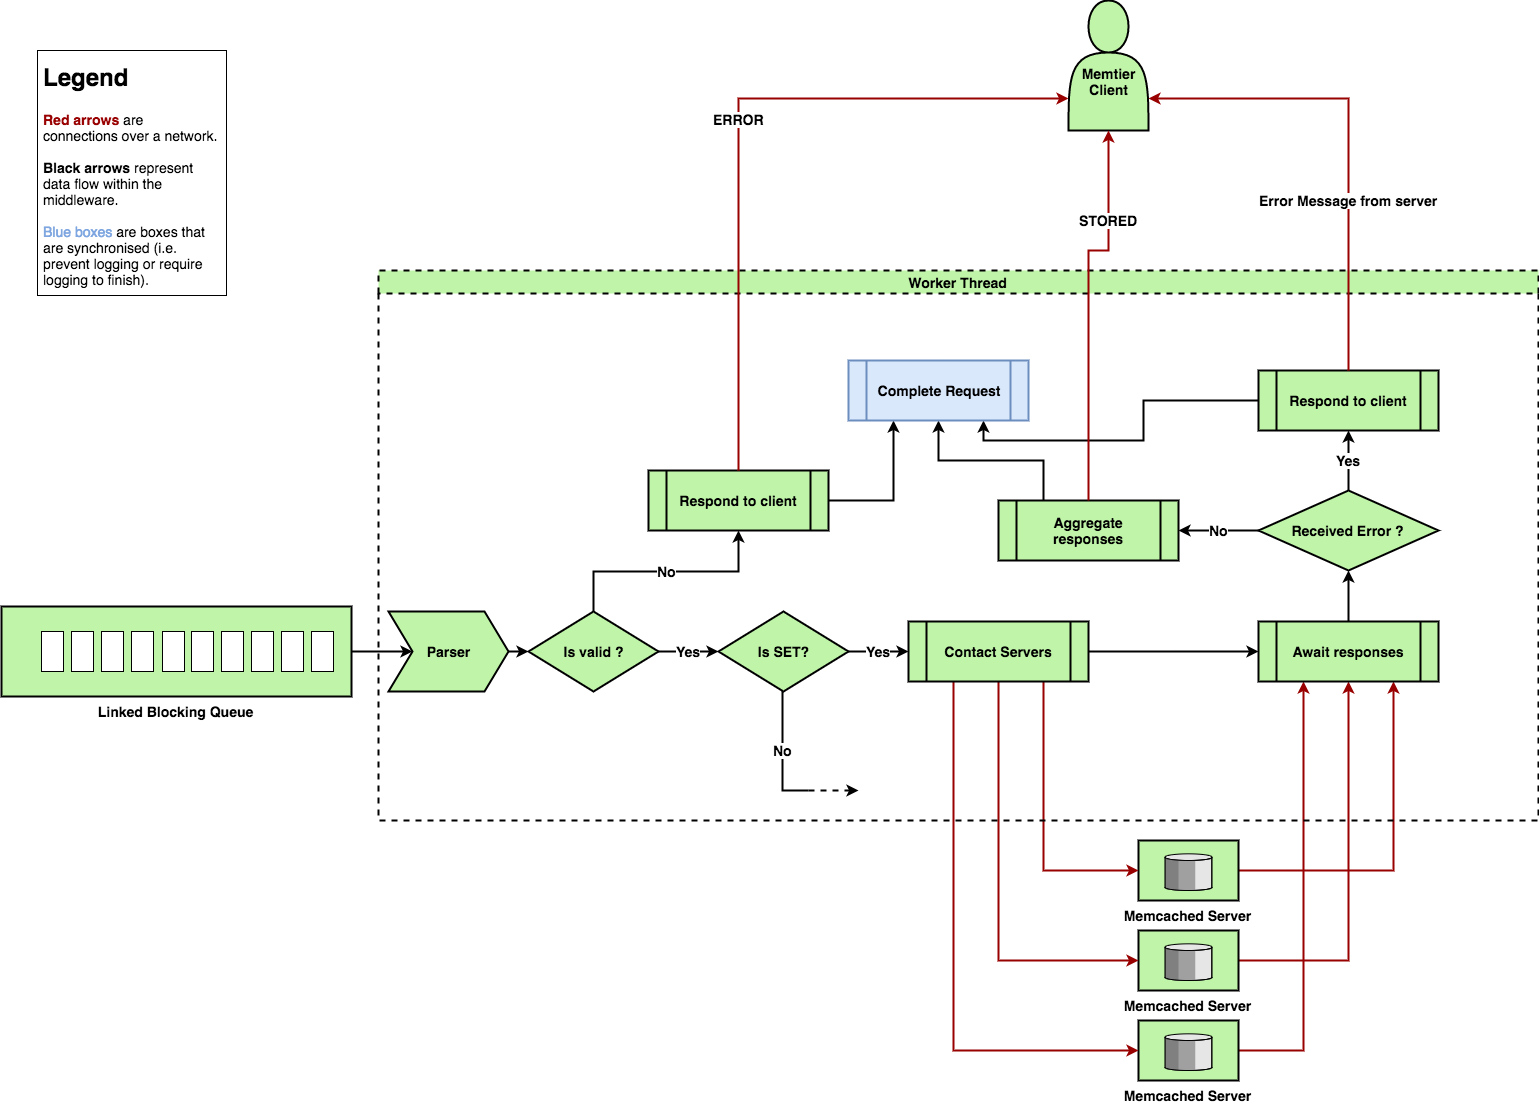
\includegraphics[width=\textwidth]{processing/graphics/sets_handling.png}
    \caption{Handling of \mintinline{java}{SET} requests}
    \label{png::sets_handling}
\end{figure}
In the case of a hit (i.e. all servers responded \mintinline{java}{"STORED\r\n"}), this is relayed to the client and the request is completed. Request completion will be described under logging and thread synchronisation below.

Note that that during the time the request is handled, the appropriate timestamps are updated for the request.

\subsubsection{Gets and Non-Sharded Multigets}
As these requests are not sent to all memcached servers, load balancing is in order. To perform load balancing, a server is chosen by simply taking the least recently used server across all workers. Of course, this can be suboptimal if the least recently used server is still working on a large request and other servers have already freed after handling smaller requests. However, due to relatively strong variations in the network latencies, it is very difficult to predict the time needed for a server to process a request as these latencies account for the majority of the server time.

\begin{figure}[h]
    \centering
    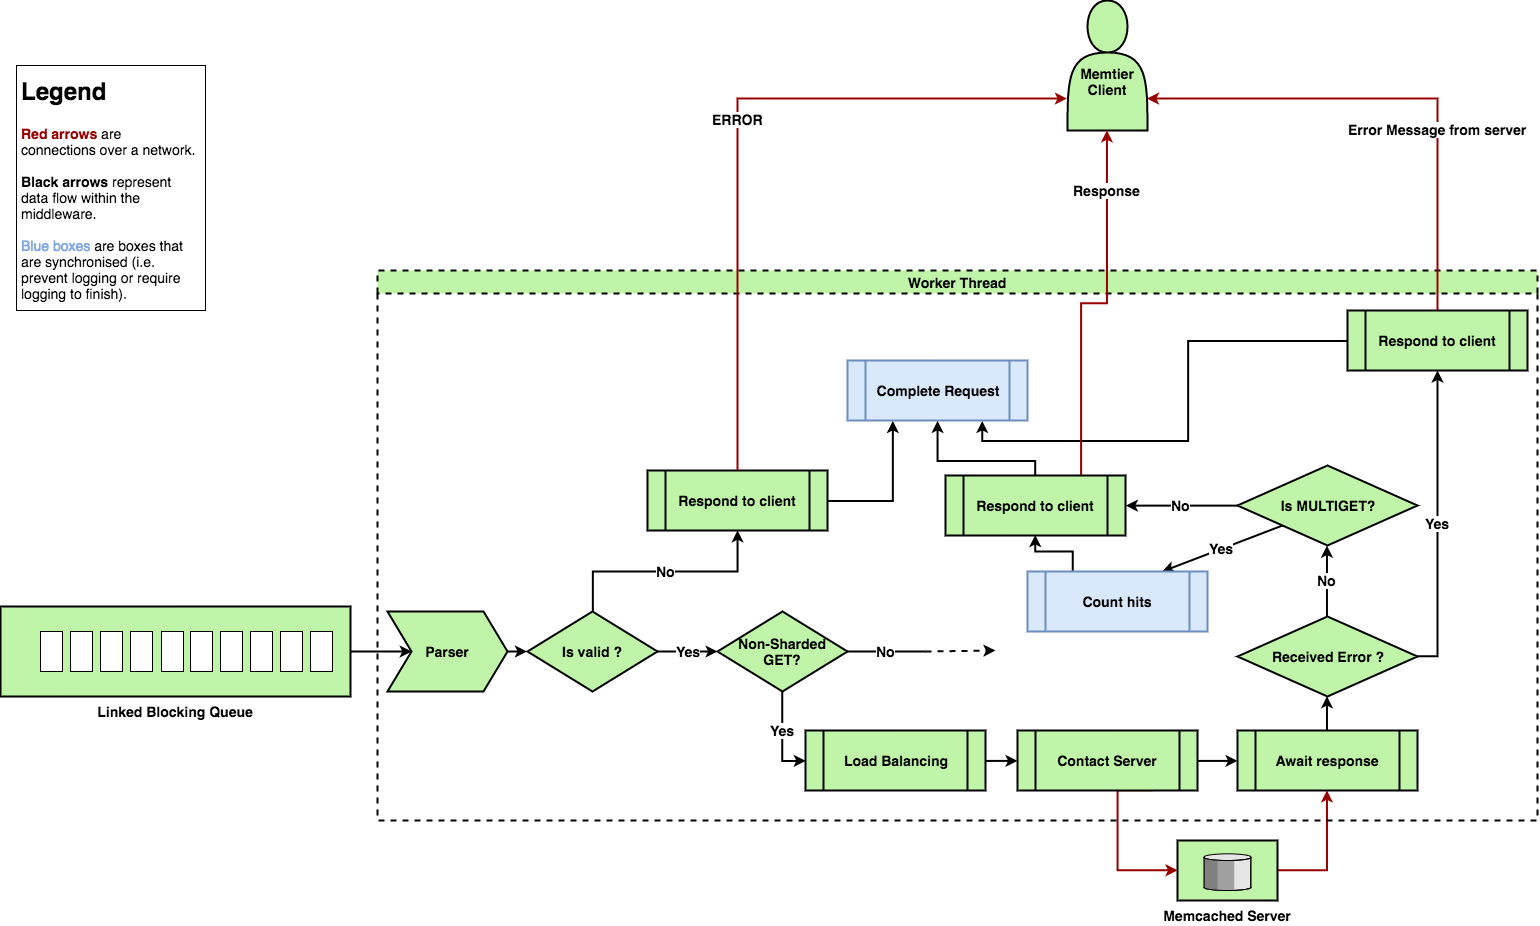
\includegraphics[width=\textwidth]{processing/graphics/gets_handling.png}
    \caption{Handling of \mintinline{java}{GET} and non-sharded \mintinline{java}{MULTIGET} requests}
    \label{png::gets_handling}
\end{figure}

The request, as it was received by the client, is then sent to the selected server. The worker awaits a answer and continuously reads from the channel until the response either ends with \mintinline{java}{"END\r\n"} or matches an error (anything ending with \mintinline{java}{"ERROR\r\n"}, i.e. also \mintinline{java}{"SERVER_ERROR\r\n"} or \mintinline{java}{"CLIENT_ERROR\r\n"}). Note that this does not create a hot loop as the channel reading is blocking.

If the request is of type \mintinline{java}{multiget}, the worker checks how many values were included in the response compared to the number of values requested in the command. This then determined the number of hits and misses of the request.

For a \mintinline{java}{get}, the response is compared to \mintinline{java}{"END\r\n"} and checked if it ends with \mintinline{java}{"ERROR\r\n"}. If neither is the case, the request is flagged as a hit.

Both for \mintinline{java}{multigets} and single \mintinline{java}{get}, the response is then relayed to the client and the request completed.


\subsubsection{Sharded Multigets}
In the case of a sharded \mintinline{java}{multigets}, the \mintinline{java}{readSharded(request, response_buffer, temp_buffer)} function is called. This function completely takes care of the handling of such requests with the exception of request completion. Sharded requests are handled in two ways (graphically shown in figure \ref{png::multigets_handling}):
\begin{enumerate}
    \item If the number of requested values is less than the number of available memcached servers, load balancing is performed and a single \mintinline{java}{get} is sent to a server. Again, the servers responses are interpreted in the same order as the servers were contacted. If an error is received from any server, \mintinline{java}{"ERROR\r\n"} is relayed to the client and the server channels are cleared for the next request. Otherwise individual responses are read into the temporary buffer, \mintinline{java}{"END\r\n"} is removed from the end of the buffer and the entire buffer is appended to the response buffer.
    \item If the number of request values is larger than the number of available memcached servers, no load balancing is required as all servers will need to be contacted anyways. The processing is then performed as above.
\end{enumerate}
\begin{figure}[h]
    \centering
    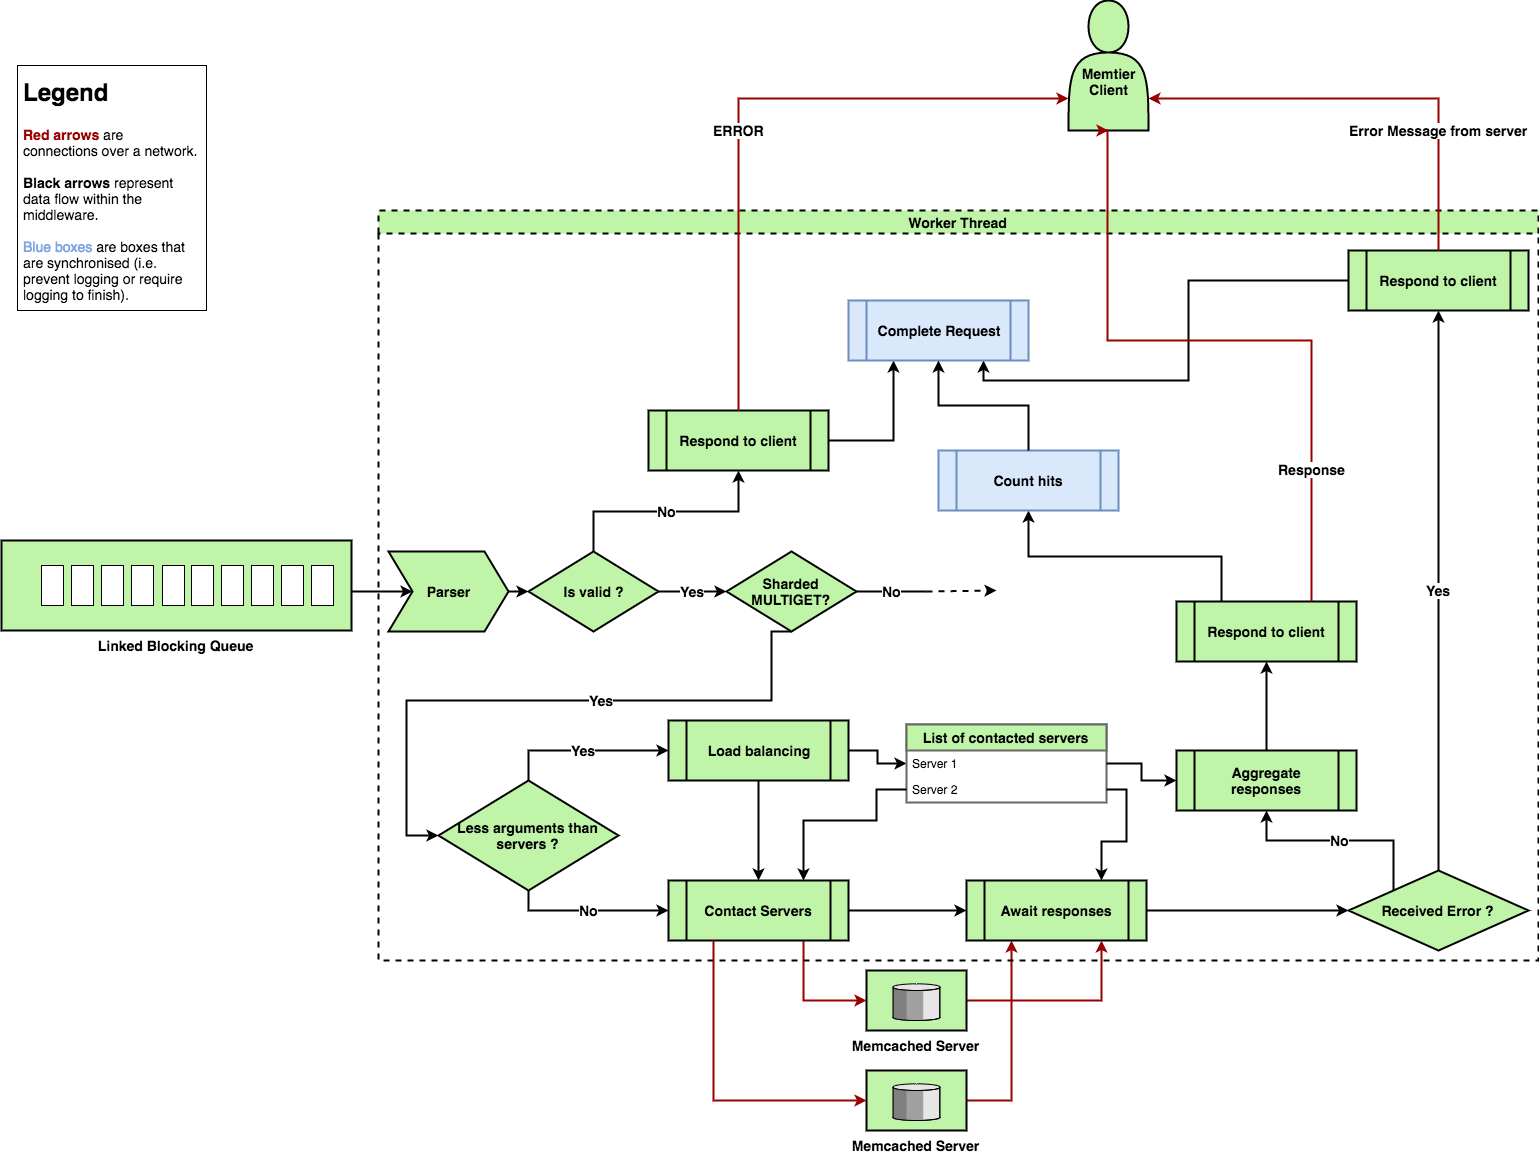
\includegraphics[width=\textwidth]{processing/graphics/multigets_handling.png}
    \caption{Handling of sharded \mintinline{java}{MULTIGET} requests}
    \label{png::multigets_handling}
\end{figure}
When all memcached servers have answered, \mintinline{java}{"END\r\n"} is added to the response buffer and the response is relayed to the client unless an error occurred in one of the servers. The response buffer is then converted into a string to check the number of hits. Note that this is performed irrespective of a server responding \mintinline{java}{"ERROR\r\n"}.


\subsection{Logging, Request Completion and Thread Synchronisation}
All statistical data relating to a request is stored within the request itself, hence the reserved fields for timestamps, type and hit flags. When a request is completed, the \mintinline{java}{complete(request)} private method of that worker object is called. This method then computes the required statistics and stores them internally in the corresponding worker object. Therefore, up until the completion of the request, no internal data of the worker was touched with the exception of \mintinline{java}{multigets} hit counting.

Every part of the workers that accessed internal statistics data is synchronised with respect to the worker object. Hence both the \mintinline{java}{complete(request)} and the \mintinline{java}{multiget} hit counting are synchronised. This ensures memory consistency when accessing the internal statistical data for logging. Thus all data should be consistent and no request should only be partially logged unless the logger kicks in between two blue boxes in figures \ref{png::gets_handling} and \ref{png::multigets_handling}. This can only happen during the handling of multigets and creates hits to be registered even though the request is incomplete. This is very unlikely to happen since close to no work is performed between any two blue boxes. Moreover, note that this does not affect any final statistics.

The logging is performed by a static function:
\begin{minted}{java}
    public static String getRecord(ArrayList<Worker> workers, int queueLength);
\end{minted}
(of the worker class) that, when accessing the internal data of a worker in its argument list, locks that worker, hence preventing it from modifying its internal statistical data. This is done in order to get consistent interval information when logging. \\
Every second, the \mintinline{java}{getRecord()} function is called on all workers and gathers their statistical data to output what has happened in the last second. Note that this does not prevent the worker from performing work until it reaches either request completion or a multiget hit count update. Due to the fact that data gathering is relatively fast compared to the overall time needed to process a request and the server time, this usually does not affect performance. Moreover, note that not all workers are blocked, but only the one currently being accessed. This can create slightly offset data when the middleware is launched with a large number of workers as the last few workers might complete some requests while the data from the first worker is being read. However, this only affects the time interval, not the overall data, because the logger only gathers data from when \mintinline{java}{getRecord()} was called \textit{on that worker}. Hence, even if the last worker completes more requests while the data from the first worker is being collected, these completed requests will not be considered the next time \mintinline{java}{getRecord()} is called on that worker.

Furthermore, \mintinline{java}{getRecord()} also takes care of clearing any histogram information stored in workers when running for the first time. This is to ensure that histogram data does not include requests completed during warm up time. The warm up time is set to ten seconds, therefore \mintinline{java}{getRecord()} is called ten seconds after the launch of the middleware and then again every second after that. This is performed by a scheduled executor service spawning a thread from the net-thread.

The analysis data is logged both to console and to an \mintinline{shell}{analysis.log} file in the home directory. Note that the logs in the log file additionally contain timestamps. Moreover, the middleware logs system information such as interruptions, errors setting up sockets, connection request, etc. to \mintinline{shell}{system_report.log} also in the home directory.

On top of that, when the \mintinline{java}{ShutdownHook} is triggered, statistics for individual workers is gathered and the histogram is printed. The statistic for individual workers include queue time, processing time, server time, total count, hits per second and misses per second for each request type. The final statistics layout is very similar to the one provided my memtier.

\subsection{Terminology}
This section describes the terminology used across all experiments unless explicitly specified otherwise.
\begin{description}
    \item[Response time/latency as given by middleware]\hfill\\ This refers to the time between creation of a request when read from the server socket to the time the request is completed (i.e. the response has been sent to the client). Thus, this does not include the time the request and response spend in the network between the client and middleware hosts.
    \item[Processing time]\hfill\\ This refers to \textit{all} time between the moment a request is dequeued and the moment the request is completed. Hence this fully includes server time.
    \item[Server time]\hfill\\ Server time refers to the time between the moment a request is forwarded to \textit{any} memcached server and the time a response has been received from \textit{all} necessary memcached servers. Therefore, in the case of sharded \mintinline{java}{multigets} and \mintinline{java}{sets}, it is measured from just before the first server is contacted to just after the last response is received. Note that this also includes network latencies between middleware and servers.
    \item[Standard deviation]\hfill\\ Unless explicitly stated otherwise, the standard deviation is the deviation between the average \textit{interval} measurements of some specific software. These intervals are always one second in length. Hence the standard deviation of the latencies measured by 2 clients is the deviation of the results obtained from taking, each second, the average latency measured by both clients. The purpose of this is to show the deviation of the overall system from it's mean behaviour over the experiment time window.
    \item[Server]\hfill\\ A machine running an instance of memcached.
\end{description}

\subsection{Overall Experimental Design}
All repetitions taken are at least 90 seconds long. The ten first seconds are evicted (warm up time) and the 80 next measurements are taken as the data. For client and server data, only the first eight seconds are evicted as the automation scripts allow two seconds for the middleware to boot properly before launching the clients. Note that due to \mintinline{java}{ssh} network latencies, the 80 second windows of measurements might not perfectly coincide between clients, middleware, and servers, but this should be insignificant compared to the overall length of a repetition. The effect of this can be seen in the slight differences of throughput between client and middleware data. However, as will be shown in the first middleware baseline, this is an irrelevant difference.

The error bars used for all graphs are obtained from the standard deviation as described in the terminology subsection above. Deviation of the averages across repetitions are also available in the final data sheets (\mintinline{shell}{/processing/final/<experiment_name>/data.csv}) but will not be used unless relevant. This would be the case if one repetition is deviating from the average significantly.

On top of that, on all memcached host machines, memcached is always launched on a single thread for all experiments.

In order to have a better understanding of system resource bounds and usage, two other pieces of software are used. Firstly, \mintinline{java}{dstat} is launched for each repetition in order to monitor CPU usage, network sends and receives, and disk reads and writes. This allows for a better overview of resource usage. Secondly, \mintinline{java}{iperf} is run at the very beginning of the experiments to measure network bandwidths between machines. This is only run once at the very beginning as all experiments were performed in a single run. Performing all experiments in one go ensures consistency in latencies between machines as no machines are reallocated between different experiments. In order to have an idea of these latencies, \mintinline{java}{ping} is also run between machines before each experiment for about five seconds. \mintinline{java}{ping} is not run during the actual experiments as it sends packets over a network which is the bottleneck for most test scenarios. Hence running it during experiments would restrict the middlewares performance even further.






\newpage

\section{Baseline without Middleware}
The experiments under this section are performed without a middleware. The purpose of this is to establish some benchmark to determine the behaviour of memtier and memcached. For both read-only and write-only workloads, client ranges from two to 56 \textit{per thread} were chosen. In the first experiment, a single memcached machine was connected to three client machines, all of which running on two threads.\\
In the second experiment, a single client machine running two instances of memtier was attached to two server machines. Both instances of memtier running on a single thread.

\subsection{One Server}
This experiment deals with the performance of memcached. Three client machines running memtier with two threads each are connected to a single memcached machine. Figure \ref{png::bench_memcached_through-clients} shows the throughput of read-only and write-only requests with respect to the total number of clients.

\begin{figure}[!h]
    \centering
    \begin{minipage}[b]{.45\textwidth}
        \centering
        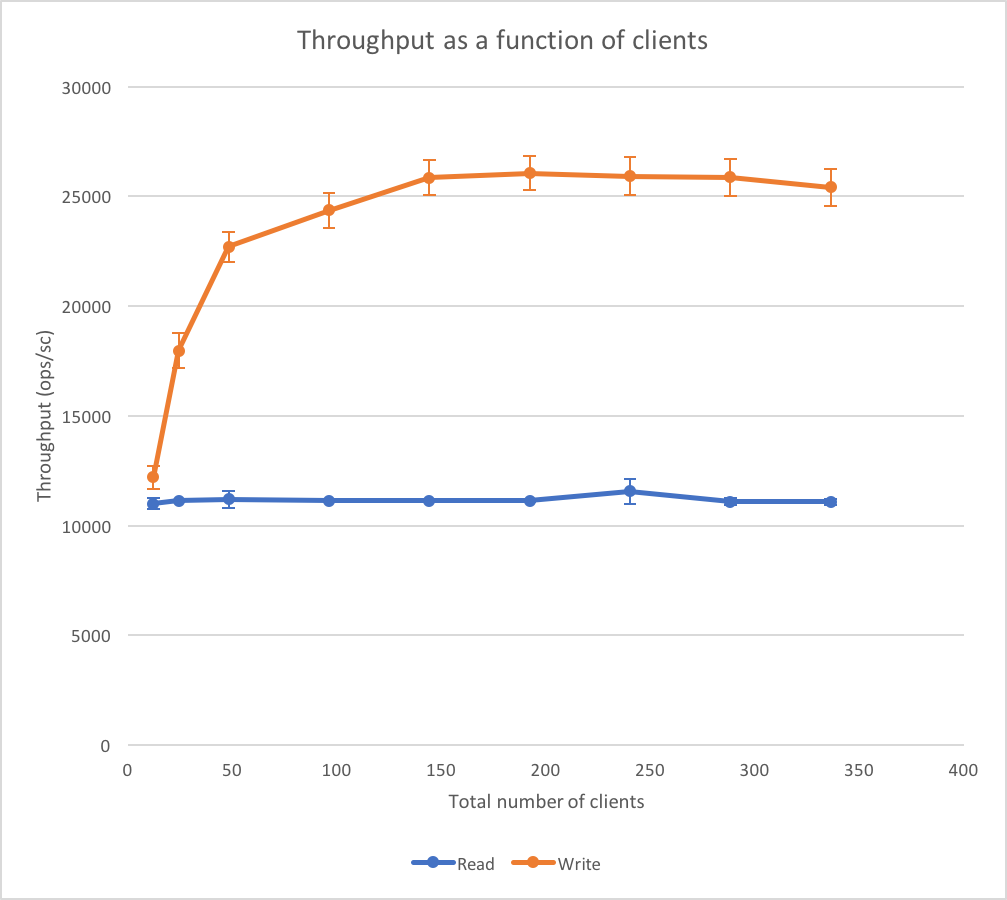
\includegraphics[width=\textwidth]{processing/graphics/bench_memcached_through-clients.png}
        \caption{Throughput as a function of total number of clients}
        \label{png::bench_memcached_through-clients}
    \end{minipage}
    \qquad
    \begin{minipage}[b]{.45\textwidth}
        \centering
        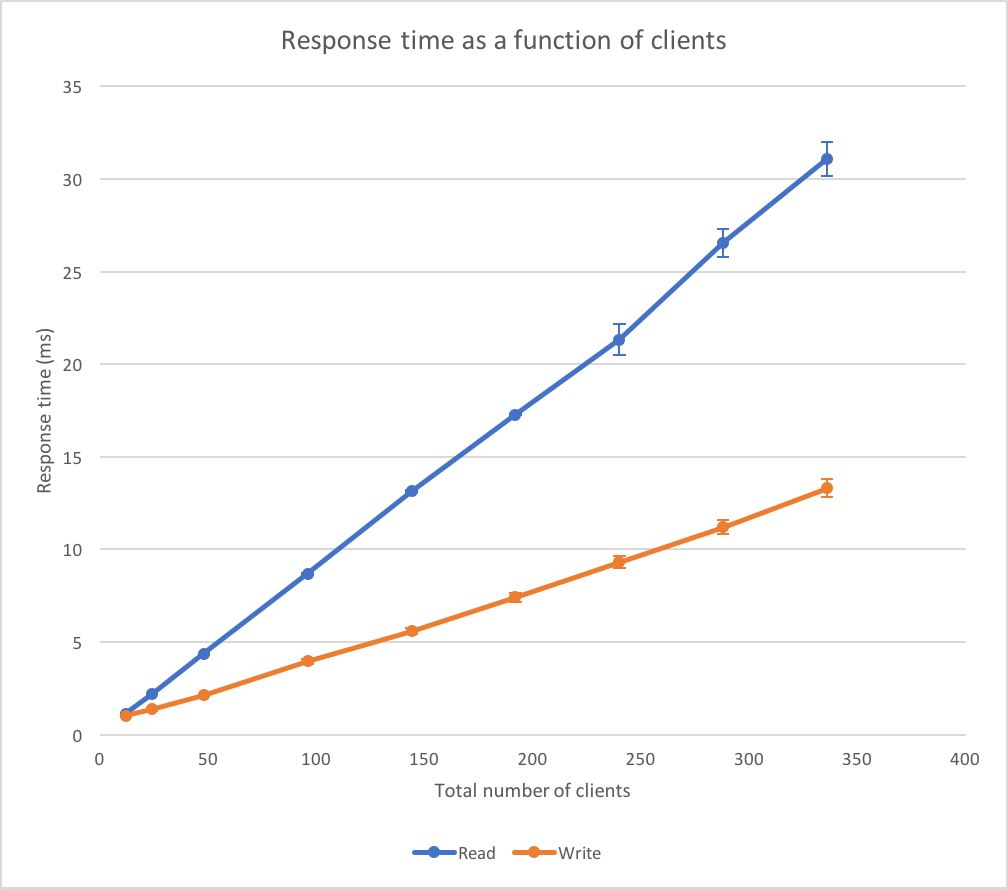
\includegraphics[width=\textwidth]{processing/graphics/bench_memcached_latency-clients.png}
        \caption{Response time as a function of total number of clients}
        \label{png::bench_memcached_latency-clients}
    \end{minipage}
\end{figure}

Figure \ref{png::bench_memcached_latency-clients} shows the respective response time with respect to total number of clients.



\subsubsection{Explanation\label{section::computation_reads}}
First, note that the experiment obeys the interactive law. This can be seen in figure \ref{png::bench_memcached_inter_law}. The response time logged by the clients coincides perfectly with the response time computed by the interactive law. Graphs illustrating the interactive law will not be shown in later experiments unless the measurements used to graph throughput and response time do not obey operational laws.
\begin{figure}[!h]
    \centering
    \begin{minipage}[b]{.45\textwidth}
        \centering
        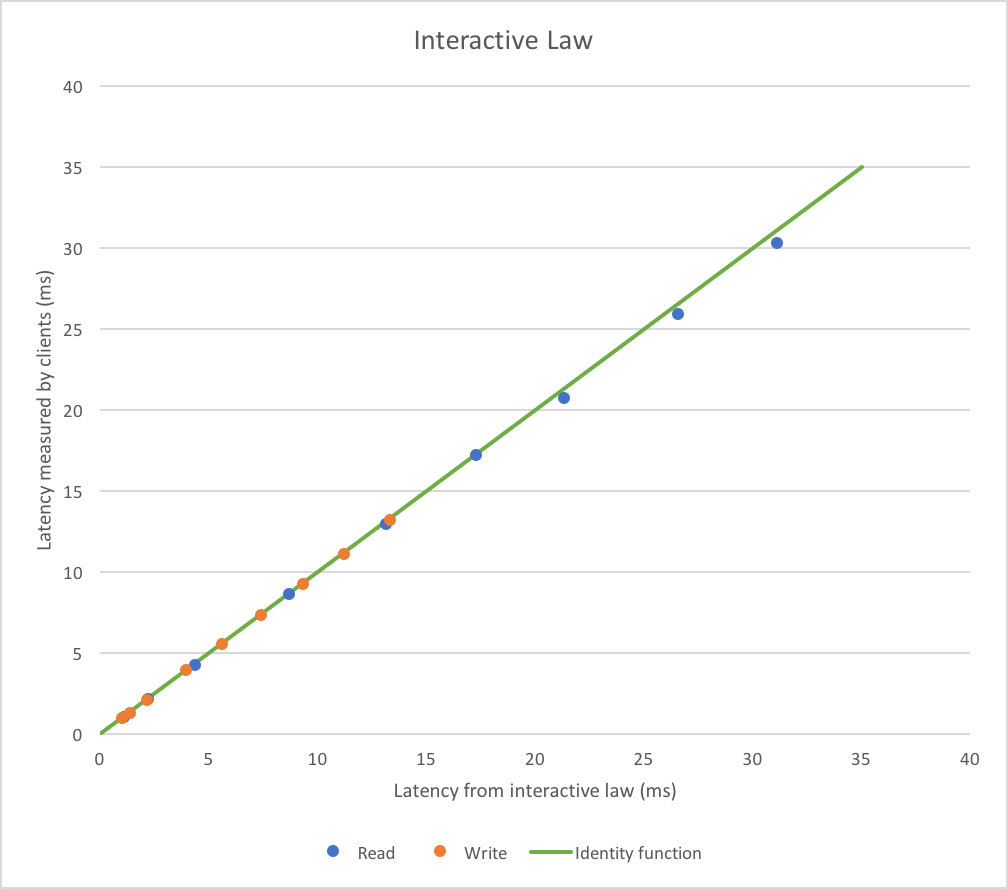
\includegraphics[width=\textwidth]{processing/graphics/bench_memcached_inter_law.png}
        \caption{Latency measured by clients versus interactive law latency}
        \label{png::bench_memcached_inter_law}
    \end{minipage}
    \qquad
    \begin{minipage}[b]{.45\textwidth}
        \centering
        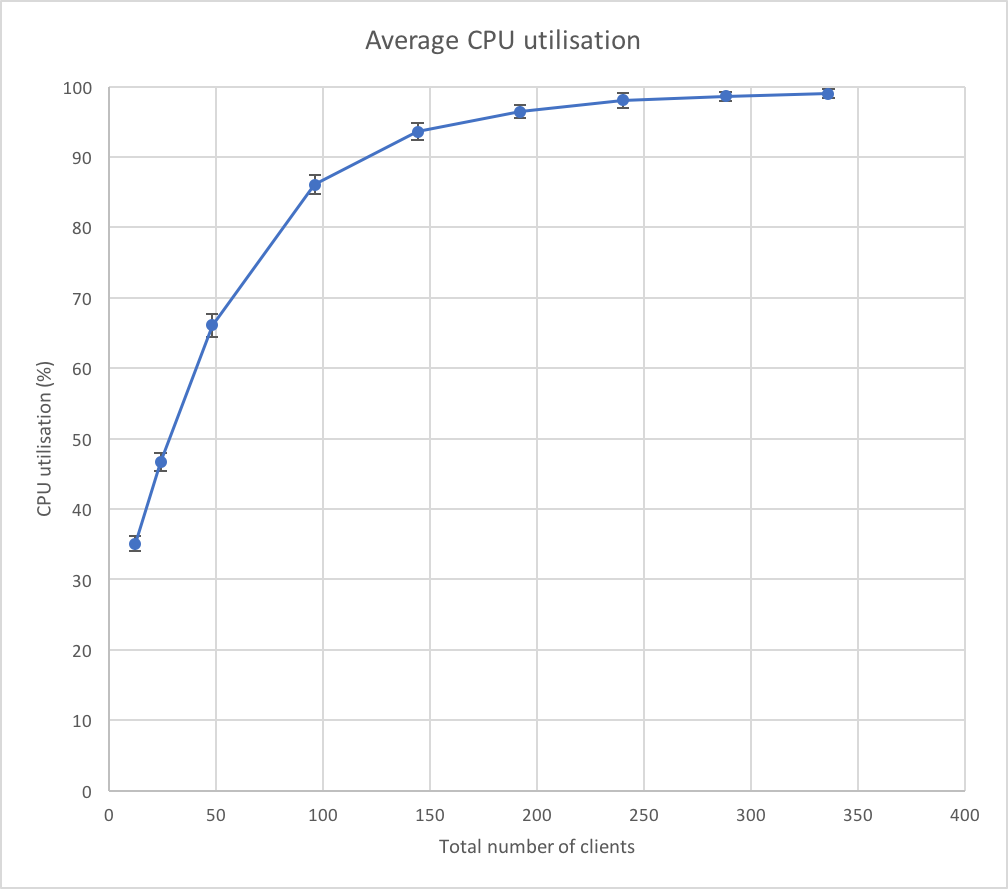
\includegraphics[width=\textwidth]{processing/graphics/bench_memcached_cpu_util.png}
        \caption{Average CPU utilisation based on total client count of memcached servers}
        \label{png::bench_memcached_cpu_util}
    \end{minipage}
\end{figure}

First consider write throughput. Memcached seems to attain saturation at around 150 clients as shown in figure \ref{png::bench_memcached_through-clients}. Figure \ref{png::bench_memcached_cpu_util} indicates that the saturation level is reached due to CPU utilisation.\\
Second, for read throughput, saturation is already reached with 12 clients total. This is due to network bandwidth. \mintinline{java}{dstat} data indicates that the average network upload of memcached is 12 megabytes per second\footnote{\mintinline{shell}{processing/final/benchmark_memcached/dstat.csv}}. From \mintinline{java}{iperf}, we know that the server upload bandwidth is also 12 megabytes per second ($96.4\text{Mbps}/8=12.05\text{MBps}$\footnote{\label{source::server_net}\mintinline{shell}{logs/server1_network.log}}). Hence memcached cannot handle more than around 11 thousand requests per second. This number makes sense since only hits occurred and data blocks are of size 1024 bytes. Then we have $11.000 \times 1024 = 11 264 000$ bytes of data uploaded to the network by the server. Note that this does not include any keys, \mintinline{java}{VALUE} and \mintinline{java}{END} statements, hence the number being slightly lower than the average network upload bandwidth measured by \mintinline{java}{dstat}.


\subsection{Two Servers}
This experiment has the goal to check for saturation levels of client machines. Figures \ref{png::bench_clients_through-clients} and \ref{png::bench_clients_latency-clients} show throughput and response time as a function of the total number of clients respectively. Note that in this case, there is no significant difference in behaviour between read-only and write-only workloads. Still the interactive law hold as shown in figure \ref{png::bench_clients_inter_law}. Note that on low ranges of response times, the response time measured by the clients is higher than the one computed by the interactive law. This is due to the fact that response times observed at low loads vary greatly between memtier instances on the same machine\footnote{\mintinline{shell}{/processing/processed/benchmark_clients/**/clients.csv}}. This is caused by different network latencies between the client machine and the two server machines.
\begin{figure}[!h]
    \centering
    \begin{minipage}[b]{.45\textwidth}
        \centering
        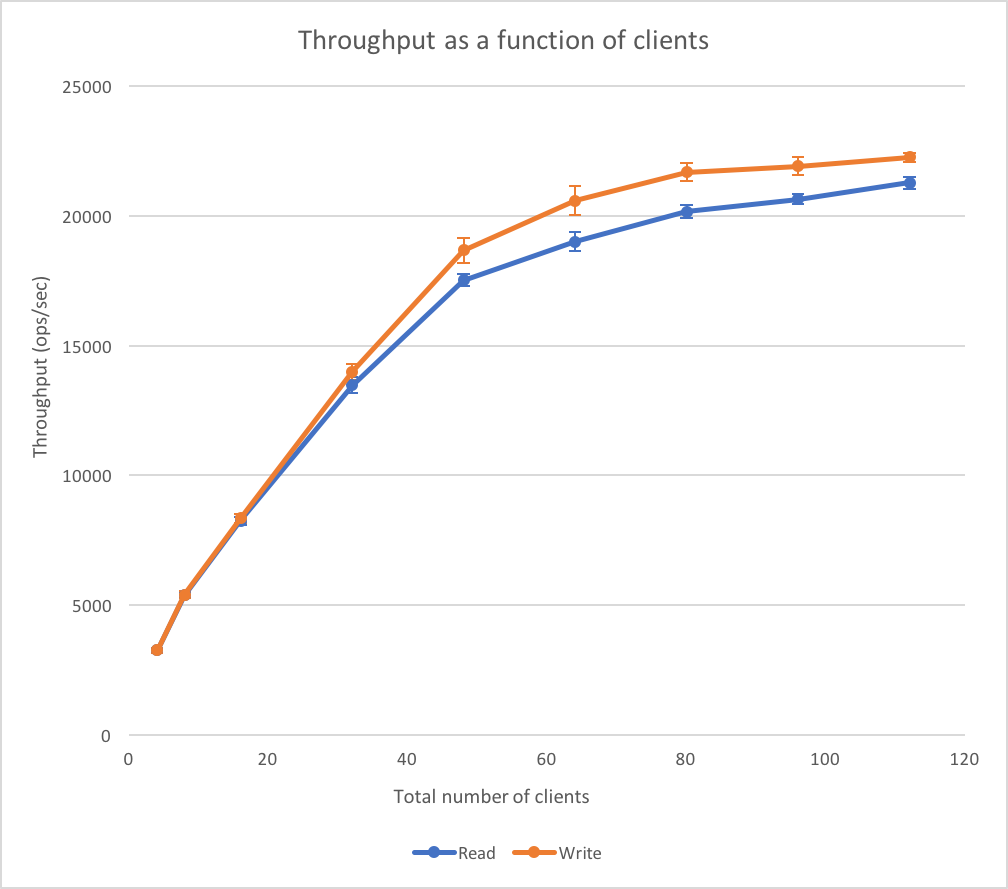
\includegraphics[width=\textwidth]{processing/graphics/bench_clients_through-clients.png}
        \caption{Throughput as a function of total number of clients}
        \label{png::bench_clients_through-clients}
    \end{minipage}
    \qquad
    \begin{minipage}[b]{.45\textwidth}
        \centering
        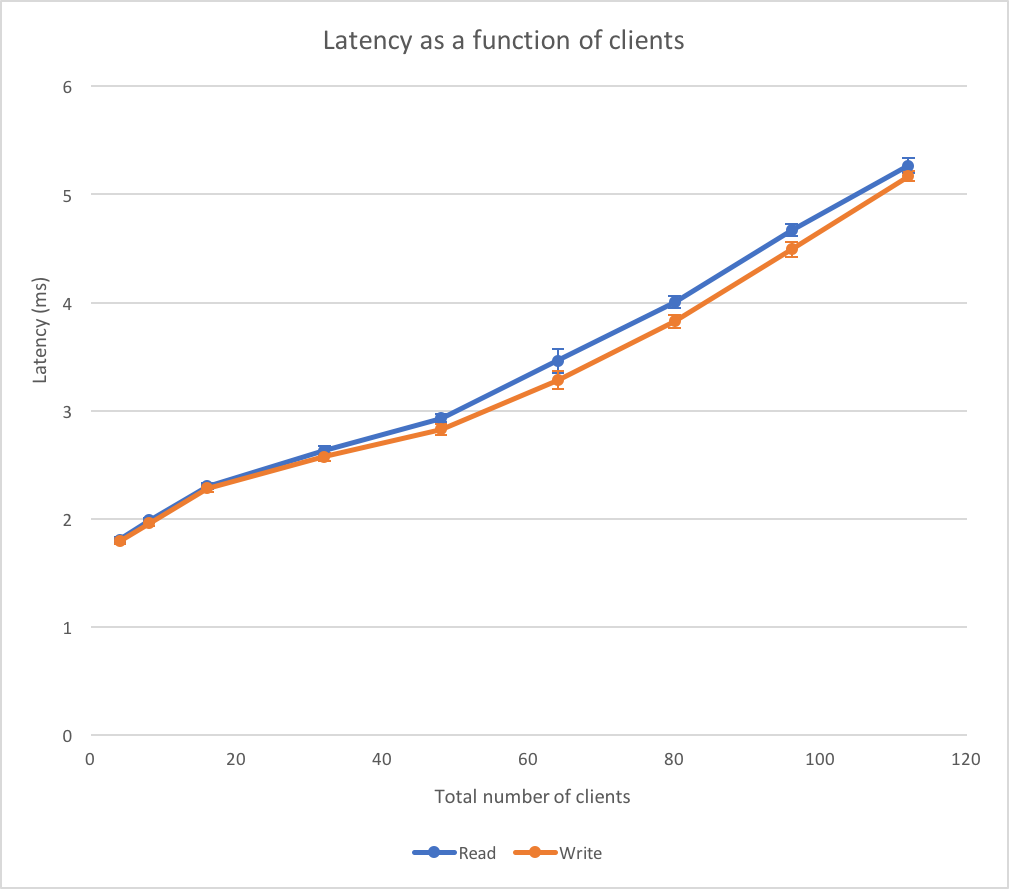
\includegraphics[width=\textwidth]{processing/graphics/bench_clients_latency-clients.png}
        \caption{Response time as a function of total number of clients}
        \label{png::bench_clients_latency-clients}
    \end{minipage}
\end{figure}

\subsubsection{Explanation}
For both reads and writes, the memtier instance connected to the first server attains maximum throughput at 24 clients per thread\footnote{\mintinline{shell}{processing/processed/benchmark_clients/**/clients_24/clients.csv}}. However, the memtier instance connected to the second instance only attains maximum throughput at 48 to 56 clients per thread\footnote{\mintinline{shell}{processing/processed/benchmark_clients/**/clients_48/clients.csv}}. This causes the dent in figure \ref{png::bench_clients_latency-clients} at 48 total clients. Beyond that point, the latency for the first instance of memtier starts to increase much more due to saturation hence dragging the average upwards. Thus, optimally, the first instance would run with 24 clients and the second one with 48 or 56 clients to achieve maximum throughput and low response time. As only configurations with the same number of clients across all memtier threads are considered, the saturation point is at a workload of 80 total clients for reads and for writes (40 clients per thread).

For any operation, the bottleneck is the network. Figures \ref{png::bench_clients_net_reads} and \ref{png::bench_clients_net_writes} show the data written to network per second for reads and writes respectively. Note that for all graphs, averages are taken across machines. Therefore, the data written to network per second given by the blue line in figures \ref{png::bench_clients_net_reads} and \ref{png::bench_clients_net_writes} is the average \textit{per server}.

\begin{figure}[!h]
    \centering
    \begin{minipage}[b]{.45\textwidth}
        \centering
        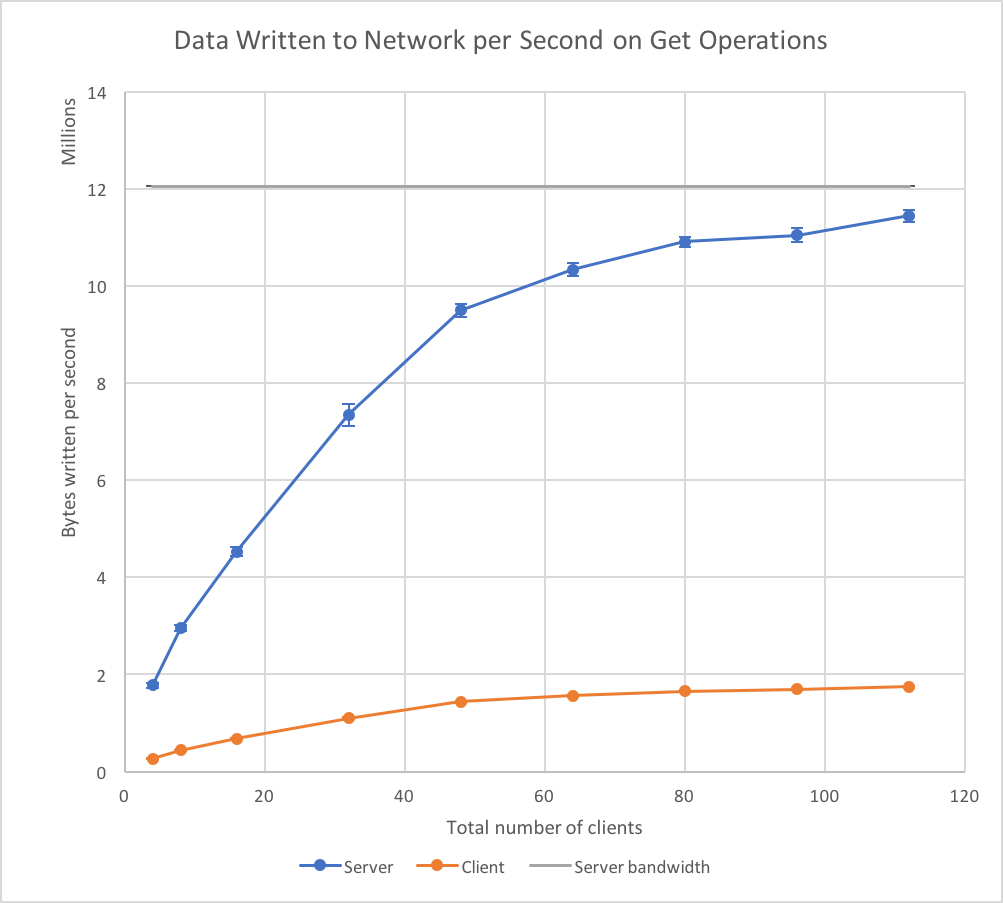
\includegraphics[width=\textwidth]{processing/graphics/bench_clients_net_reads.png}
        \caption{Data written to network per second on reads}
        \label{png::bench_clients_net_reads}
    \end{minipage}
    \qquad
    \begin{minipage}[b]{.45\textwidth}
        \centering
        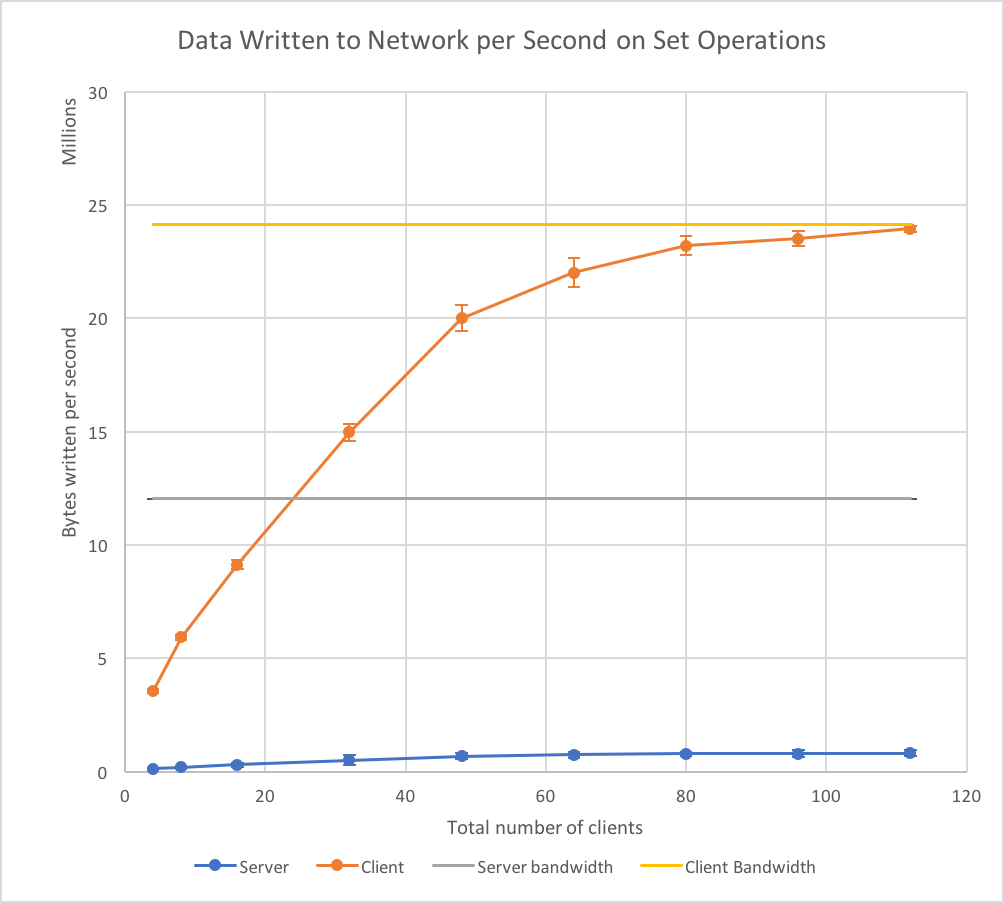
\includegraphics[width=\textwidth]{processing/graphics/bench_clients_net_writes.png}
        \caption{Data written to network per second on writes}
        \label{png::bench_clients_net_writes}
    \end{minipage}
    \begin{minipage}[b]{.45\textwidth}
        \vspace{1cm}
        \centering
        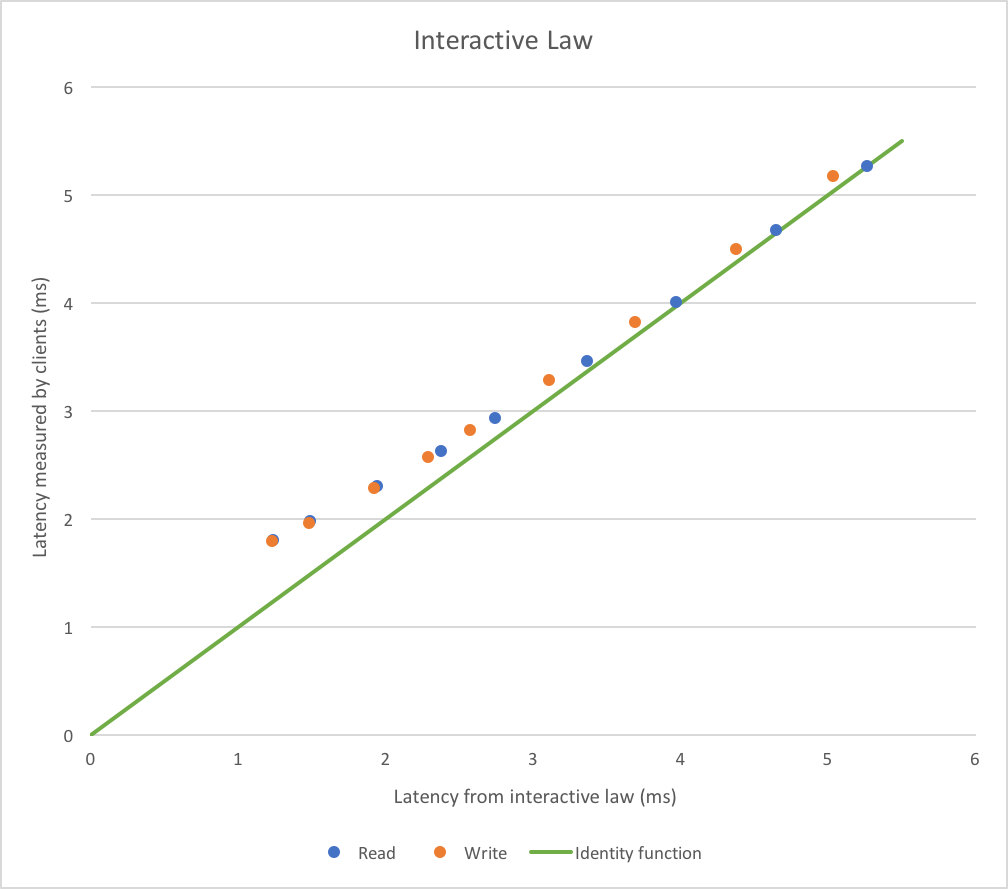
\includegraphics[width=\textwidth]{processing/graphics/bench_clients_inter_law.png}
        \caption{Latency measured by clients versus interactive law latency}
        \label{png::bench_clients_inter_law}
    \end{minipage}
\end{figure}

In the case of reads (depicted in figure \ref{png::bench_clients_net_reads}), one can see that the average data sent over the network per server approaches the bandwidth limit (12.05MB per second\footref{source::server_net}). This is the same situation as in the previous experiment.\\
In the case of writes, the maximum bandwidth for client uploads is 24.125 megabytes per second ($193\text{Mbps}/8=24.125\text{MBps}$\footnote{\mintinline{shell}{logs/client1_network.log}}). Figure \ref{png::bench_clients_net_writes} shows that this is reached relatively fast.

In conclusion, the overall bottleneck in this experiment is the network. For both reads and writes, the network does not allow the machines to reach compute power bounds.

\subsection{Summary}
In both experiments, writes generally allow to reach higher maximal throughputs (and hence lower latencies). Generally, running around 70 to 80 clients per client machines also allows to reach the highest throughput without over-saturation and increased latencies due to network bandwidth limits or server compute power bounds. The only exception to this rule is read-only workloads on a single server. In that case, the network bandwidth limit is already reached with much lower client numbers.

The numbers in table \ref{table::max_through_section_2} give the maximum measured throughputs, irrespective of when this is obtained. In the best scenario, the client number with a single server is around 150 total clients. This provides throughput very close to the numbers shown in table \ref{table::max_through_section_2} but with lower response times. Similarly, for one load generating virtual machine, around 70 to 80 clients generate enough load to achieve numbers close to the ones displayed in table \ref{table::max_through_section_2} but with lower response times than with the configuration given in the table.

\begin{table}[!h]
    \centering
    \begin{tabular}{|l|p{2cm}|p{2cm}|p{4cm}|}
        \hline                        & Read-only workload & Write-only workload & Configuration gives max. throughput \\
        \hline One memcached server   &             11 558 &              26 056 &             Write-only; 200 clients \\
        \hline One load generating VM &             21 283 &              22 264 &             Write-only; 112 clients \\
        \hline
    \end{tabular}
    \caption{Maximum throughput of different VMs}
    \label{table::max_through_section_2}
\end{table}



\newpage

\section{Baseline with Middleware \label{section::net_queues}}
In this set of experiments, one load generating virtual machine and one memcached server are used. In the first experiment, a single middleware is used as intermediary between clients and the memcached server. During the second experiment, the client virtual machine is connected to two middleware machines, each getting requests from a single thread memtier instance. Both middlewares then use the same memcached server as backend.

\subsection{One Middleware}
\subsubsection{Reads}
Firstly, figures \ref{png::bench_1mw_through-clients_read_cdat} and \ref{png::bench_1mw_through-clients_read_mdat} show that there is close to no mismatch between throughput data gathered from the client and from the middleware for read operations. The small differences in throughput are caused by the fact that the measurement windows might not coincide perfectly.

\begin{figure}[!h]
    \centering
    \begin{minipage}[b]{.45\textwidth}
        \centering
        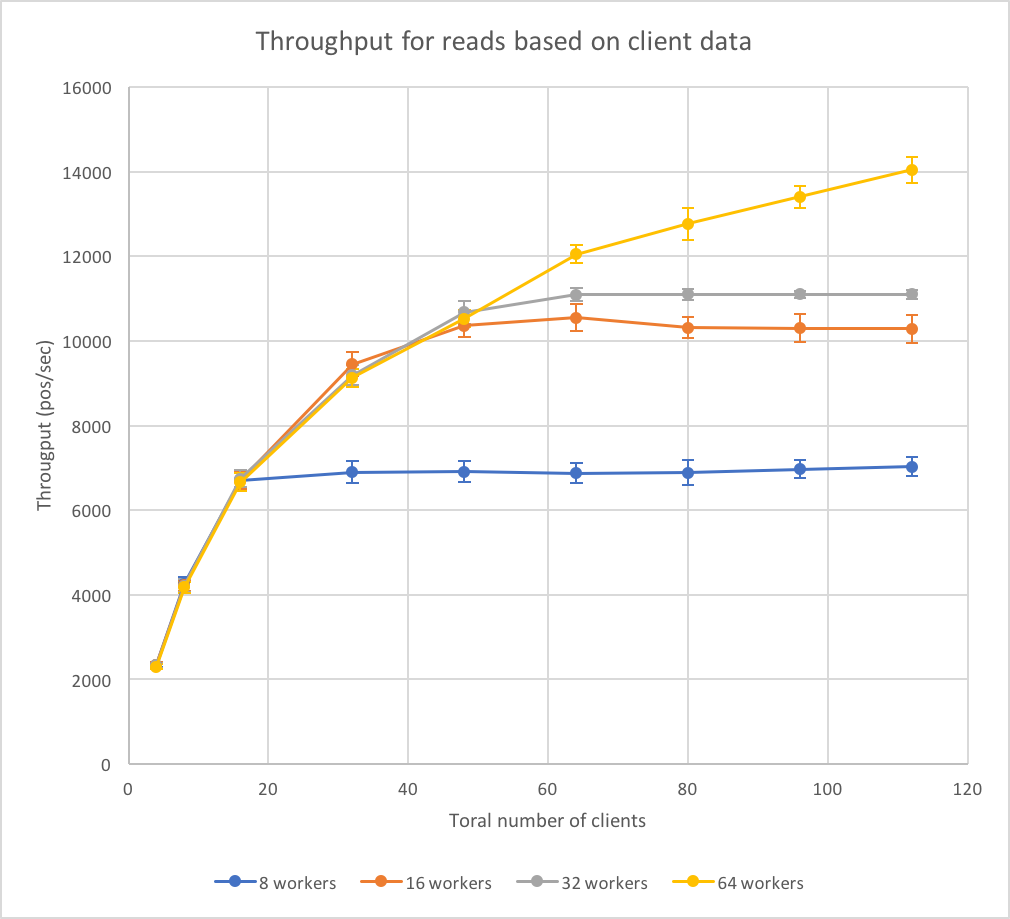
\includegraphics[width=\textwidth]{processing/graphics/bench_1mw_through-clients_read_cdat.png}
        \caption{Throughput as measured by the client machine for reads}
        \label{png::bench_1mw_through-clients_read_cdat}
    \end{minipage}
    \qquad
    \begin{minipage}[b]{.45\textwidth}
        \centering
        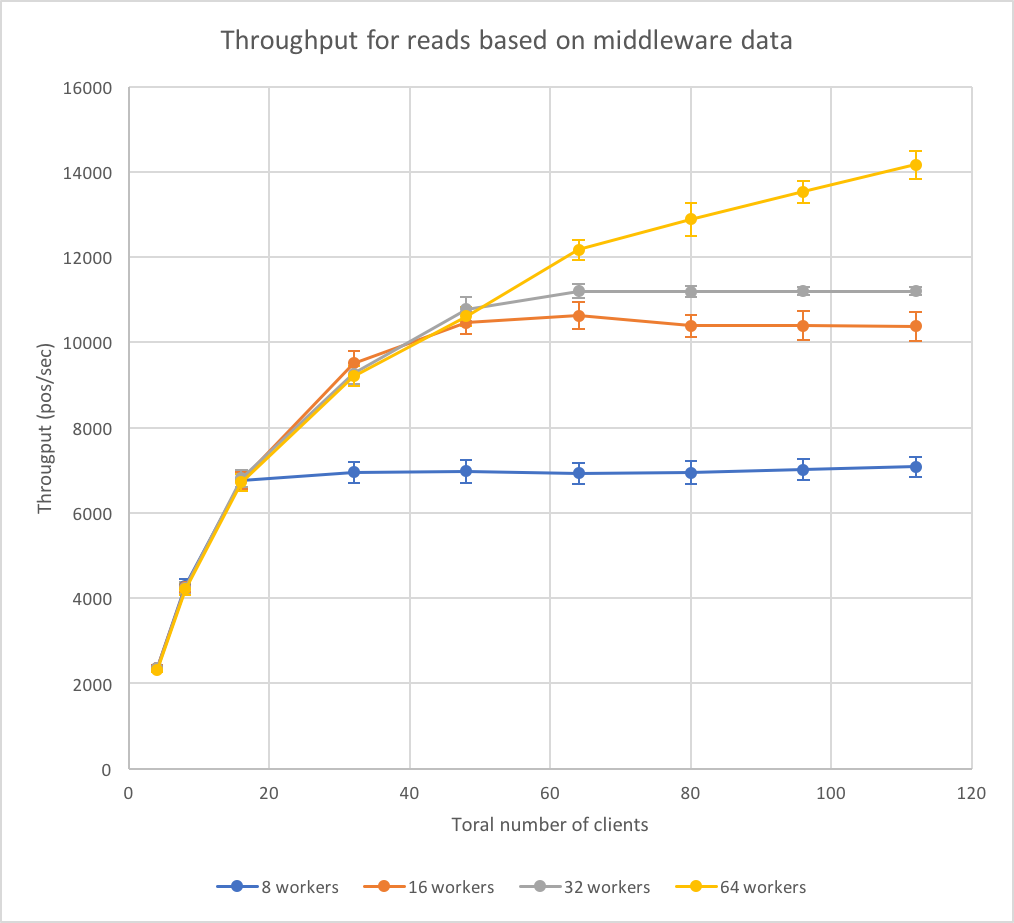
\includegraphics[width=\textwidth]{processing/graphics/bench_1mw_through-clients_read_mdat.png}
        \caption{Throughput as measured by the middleware for reads}
        \label{png::bench_1mw_through-clients_read_mdat}
    \end{minipage}
\end{figure}

Similarly, the graphs displaying response time versus total number of clients for reads shown in figures \ref{png::bench_1mw_latency-clients_read_cdat} and \ref{png::bench_1mw_latency-clients_read_mdat} are very similar. Note that there is an initial offset of about one millisecond between the data provided by the middleware and the data provided by the client. This is due to network latencies. The response time measured in the middleware is measured from the moment a request is read from the server socket up to the point the response is sent back to the client. Hence it does not include the time spend in the network by both the request before arrival in the middleware, and by the response before reaching the client. This adheres to the ping data gathered before the experiment which resulted in an average of around 0.8 millisecond network latencies between those specific client and middleware hosts\footnote{\mintinline{shell}{logs/benchmark_1mw(2017-11-17_20h58)/mw_1_ping.log}}.

\begin{figure}[!h]
    \centering
    \begin{minipage}[b]{.45\textwidth}
        \centering
        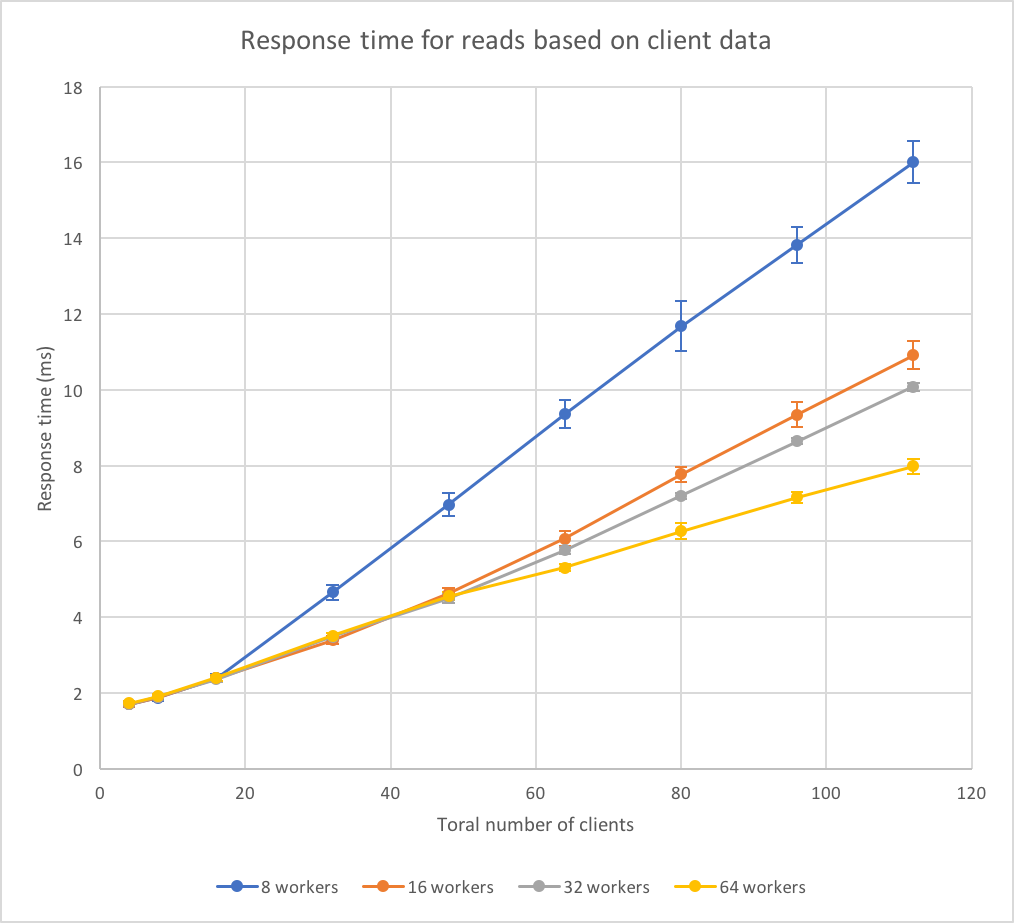
\includegraphics[width=\textwidth]{processing/graphics/bench_1mw_latency-clients_read_cdat.png}
        \caption{Response time as measured by the client machine for reads}
        \label{png::bench_1mw_latency-clients_read_cdat}
    \end{minipage}
    \qquad
    \begin{minipage}[b]{.45\textwidth}
        \centering
        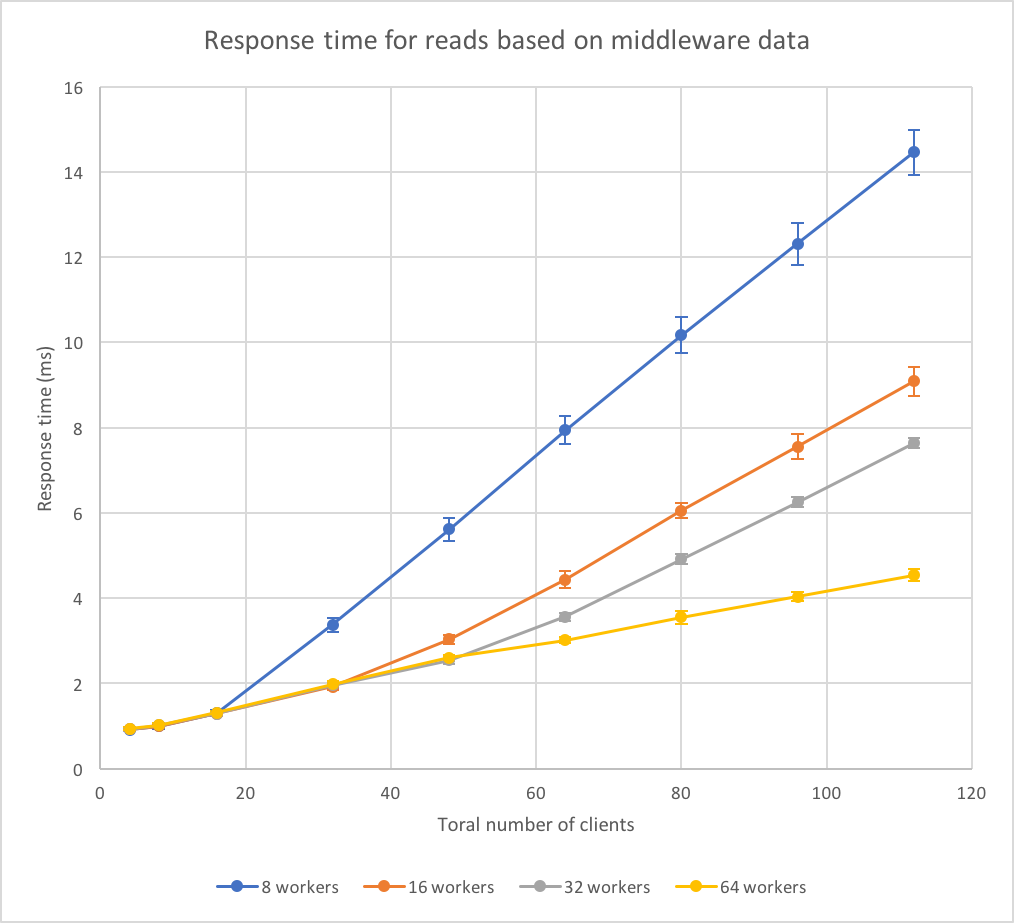
\includegraphics[width=\textwidth]{processing/graphics/bench_1mw_latency-clients_read_mdat.png}
        \caption{Response time as measured by the middleware for reads}
        \label{png::bench_1mw_latency-clients_read_mdat}
    \end{minipage}
\end{figure}

This kind of comparison between middleware and client data will not be included in future experiments. In the case of discrepancies between data aggregated by the middleware and the clients, this will be made explicit and explained. Hence no such comparison implicitly means that the data has no significant enough mismatches to require explanations.

\paragraph{8 workers}
In the case of 8 workers, the saturation is reached due to time taken to process a request, i.e. the time from the moment the request is dequeued to the time the response is sent back to the client. Note that the average time spent in the network between client and middleware (both when sending a request and receiving a response), is about one millisecond. Now note that the average time taken to process a single request when using 8 workers is also about one millisecond. Hence, as long as less two times more clients than workers are sending requests, workers are efficient enough. This can easily be seen by considering that after a worker has completed a request for a client, it will take about 1 millisecond for another request from said client to arrive in the queue (due to network latencies), during which the worker can perform exactly one other request. Hence any number of clients superior to 16 ($2\times8$ workers) will not increase throughput as all workers will necessarily already be busy. A consequence of this is increased queue times and thus increased queue lengths (as seen in figure \ref{png::bench_1mw_ql_reads}). Therefore the middleware saturates at exactly 16 clients as can be seen in figure \ref{png::bench_1mw_latency-clients_read_mdat}. Of course this number depends on the environment the middleware is used in, as shorter network latencies between middleware and servers will allow to reduce processing times, and thus higher throughputs for more clients.\\
Beyond the client number for which the middleware saturates, server times also stabilise. This is due to the fact that memcached has to handle only as many request per second as the middleware can process. This becomes constant beyond the point of saturation, hence server times become constant as well (see figure \ref{png::bench_1mw_st_reads}).

\paragraph{16 workers}
For 16 workers, we encounter the same problem as for 8 workers. However, since we now have 16 workers working concurrently, the phenomenon only occurs with a number of clients superior to 32 ($2\times16$ workers). This is obvious when looking at figure \ref{png::bench_1mw_ql_reads}. As a direct consequence of this, server times stabilise beyond this point (see figure \ref{png::bench_1mw_st_reads}). The change is not as drastic as with 8 workers since the probability for slight changes in network latencies to result in a worker being idle increases with the number of workers. For example, due to a slight increase in network latency, more than 16 requests might be in the network between client and middleware, hence resulting in at least one worker being idle (by pigeonhole principle) if only 32 clients are used.

\paragraph{32 workers}
With this configuration, the network bandwidth becomes a problem once more. With 48 total clients, the memcached server has already nearly reached the network bandwidth limit. Again, this is can be computed manually as in section \ref{section::computation_reads}. As the throughput reaches levels close to 11k reads, the network becomes the bottleneck.

\paragraph{64 workers}
Note that this data is skewed. Obviously, if for 32 workers the network bandwidth was a bottleneck, increasing the number of worker should not increase throughput as indicated in figure \ref{png::bench_1mw_latency-clients_read_mdat}. The reason that throughput can increase beyond the levels without middleware is the following. The experiment was run on a rather large range of clients and all read repetitions were performed collectively. Hence during several hours the only operations sent to memcached were reads, this resulted in all cached data being evicted while running the experiment with 64 workers. Table \ref{table::data_eviction} shows at what point exactly the data was evicted.

\begin{table}[!h]
    \centering
    \begin{tabular}{|l|l|r|r|r|}
        \hline Ratio & Sharded & Workers & Client per thread & Hit/request ratio \\
        \hline 0:1 & false & 64 & 2 & 1 \\
        \hline 0:1 & false & 64 & 4 & 1 \\
        \hline 0:1 & false & 64 & 8 & 1 \\
        \hline 0:1 & false & 64 & 16 & 1 \\
        \hline 0:1 & false & 64 & 24 & 0.963838567 \\
        \hline 0:1 & false & 64 & 32 & 0 \\
        \hline 0:1 & false & 64 & 40 & 0 \\
        \hline 0:1 & false & 64 & 48 & 0 \\
        \hline 0:1 & false & 64 & 56 & 0 \\
        \hline
    \end{tabular}
    \caption{Data Eviction}
    \source{/processing/final/benchmark\_1mw/data.csv}
    \label{table::data_eviction}
\end{table}

Therefore note that beyond 48 clients ($24\times2$ threads), memcached responses contain no more data, hence effectively removing the network bandwidth bound. In fact, average network sends per second are reduces from 11MB to slightly more than 8MB\footnote{\mintinline{shell}{processing/final/benchmark_1mw/dstat.xlsx!Sheet1}} per second even though throughput rises as indicated by figure \ref{png::bench_1mw_through-clients_read_mdat}. This also causes queue lengths to increase slower than normally as more requests per second can be handled by memcached. This can be seen in figure \ref{png::bench_1mw_ql_reads}. In the case of server times, they are first reduced due to less data having to be sent over the network, then increase beyond the level of 32 workers (figure \ref{png::bench_1mw_st_reads}) simply because much more requests have to be handled by memcached, hence increasing response time of the server. Normally, if the data eviction had not occurred, throughput with 64 workers should have behaved similarly to throughput with 32 workers.


\begin{figure}[!h]
    \centering
    \begin{minipage}[b]{.45\textwidth}
        \centering
        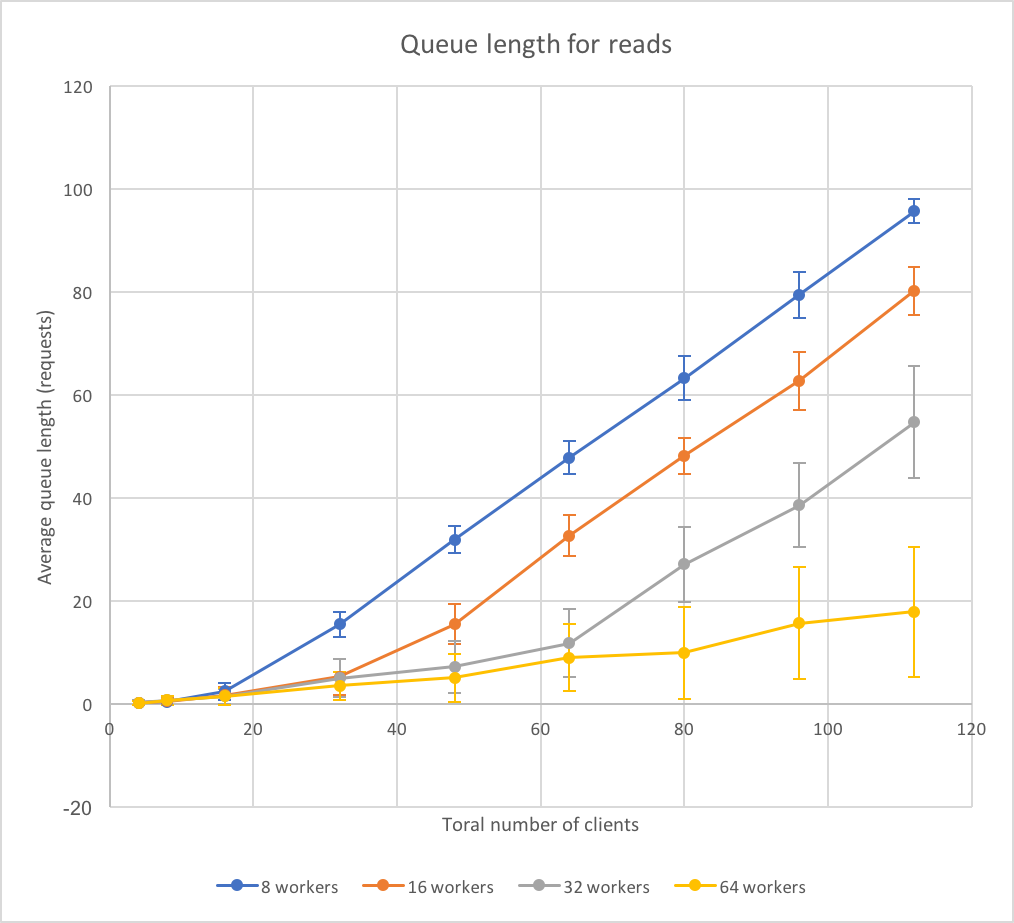
\includegraphics[width=\textwidth]{processing/graphics/bench_1mw_ql_reads.png}
        \caption{Queue length for reads}
        \label{png::bench_1mw_ql_reads}
    \end{minipage}
    \qquad
    \begin{minipage}[b]{.45\textwidth}
        \centering
        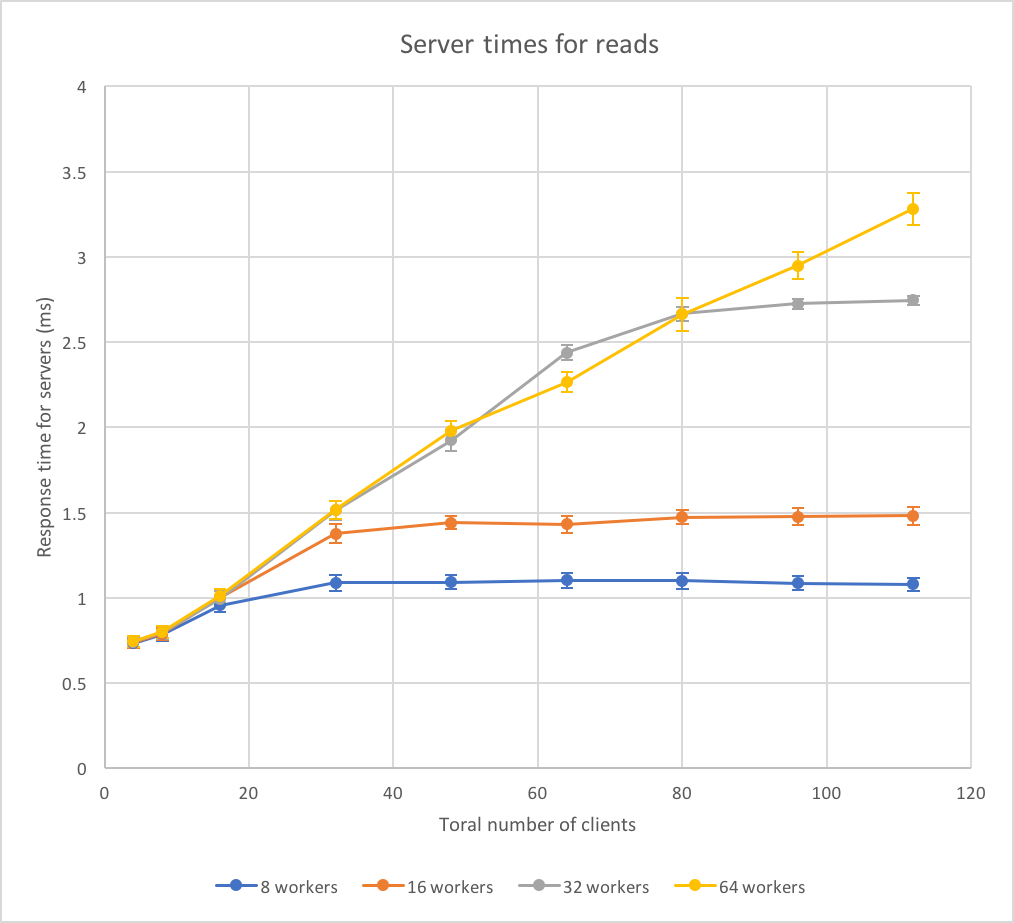
\includegraphics[width=\textwidth]{processing/graphics/bench_1mw_st_reads.png}
        \caption{Server time for reads}
        \label{png::bench_1mw_st_reads}
    \end{minipage}
\end{figure}


\subsubsection{Writes}
As discussed above, only middleware data will be shown in this section as it does not differ from client based data. Figure \ref{png::bench_1mw_through-clients_write_mdat} shows throughput as a function of number of clients for write operations. Similarly, figure \ref{png::bench_1mw_latency-clients_write_mdat} shows response time as a function of total client number for write operations based on middleware data.

\begin{figure}[!h]
    \centering
    \begin{minipage}[b]{.45\textwidth}
        \centering
        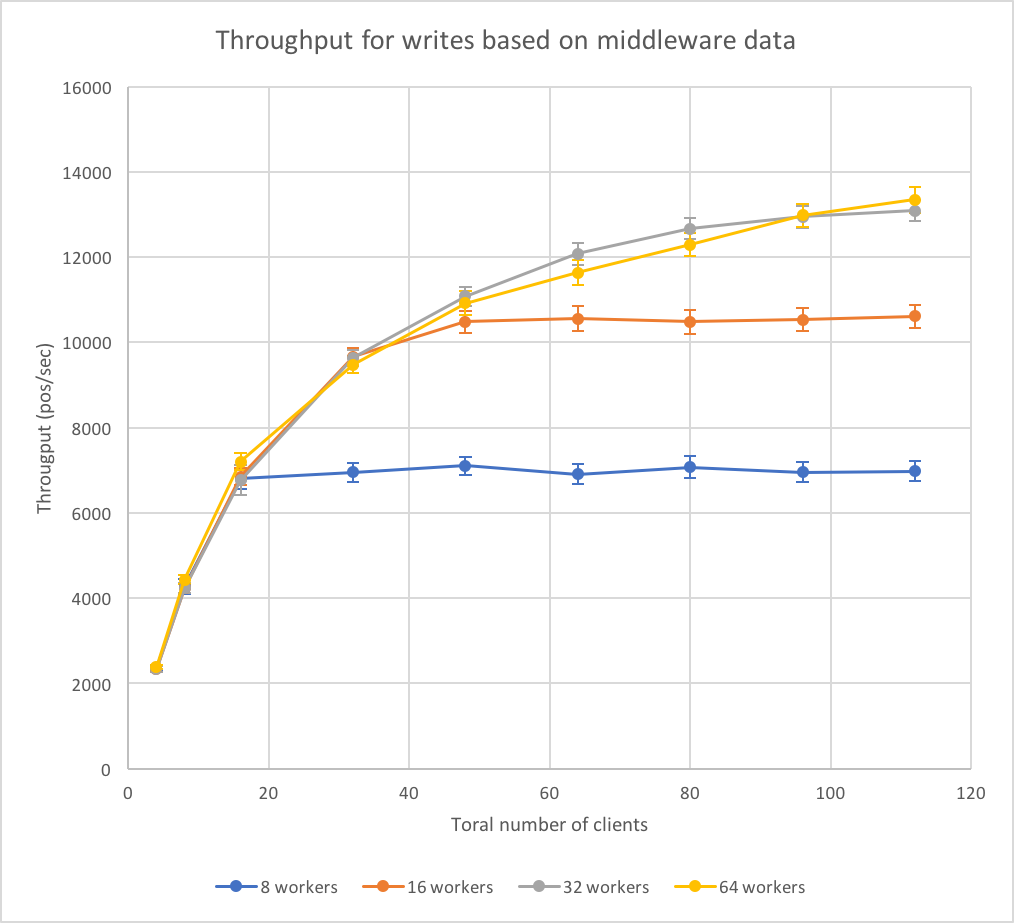
\includegraphics[width=\textwidth]{processing/graphics/bench_1mw_through-clients_write_mdat.png}
        \caption{Throughput as a function of clients for writes}
        \label{png::bench_1mw_through-clients_write_mdat}
    \end{minipage}
    \qquad
    \begin{minipage}[b]{.45\textwidth}
        \centering
        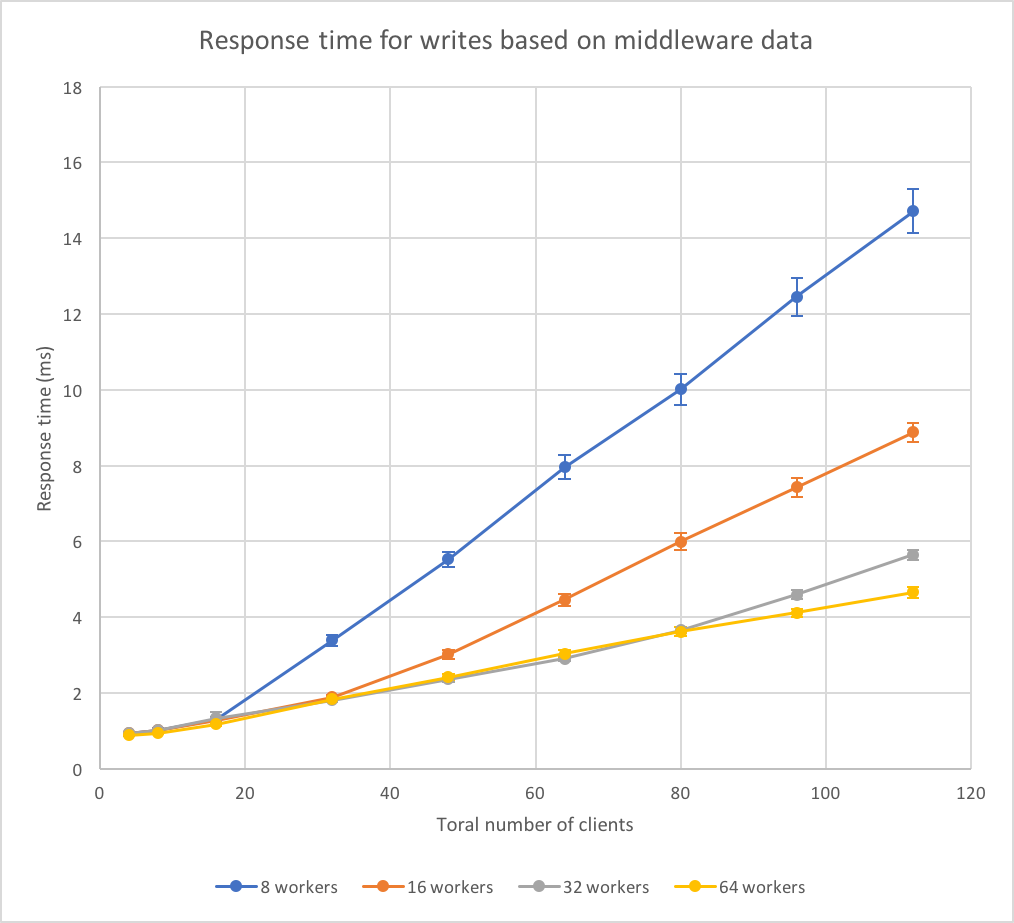
\includegraphics[width=\textwidth]{processing/graphics/bench_1mw_latency-clients_write_mdat.png}
        \caption{Response time as a function of clients for writes}
        \label{png::bench_1mw_latency-clients_write_mdat}
    \end{minipage}
\end{figure}

\paragraph{All worker counts}
With 8 workers, the same issue as for reads with 8 workers is encountered. One can clearly see in figure \ref{png::bench_1mw_through-clients_write_mdat} that past 16 clients the system is saturated. Unsurprisingly, as network latencies between client and middleware, and between middleware and server are similar to the ones for reads, the throughput attained when saturated is comparable. Note that the same problem is encountered for all worker configurations. The server response time increases as throughput increases (see figure \ref{png::bench_1mw_st_writes}), just as presented in the server baseline and shown in figure \ref{png::bench_memcached_latency-clients}. This causes increasing processing times in the middleware thus reducing the speed up by doubling worker counts. Moreover, the network latencies between client and middleware increase in parallel to this hence preserving the ratio of about 2 clients per worker before reaching saturation. For example, figure \ref{png::bench_1mw_netlat_st_64writes} shows the change in server times and network latencies between middleware and clients. Note that the network latencies are computed by taking the difference in response time measured by the middleware and the response time measured by the client machine. The increase in this latency is likely due to the fact that the net-thread in the middleware cannot read from requests from the network fast enough. Thus, when a large amount of requests arrive in very short time windows, some of the request need to wait a relatively long time before being read by the net-thread and added to the queue.

\begin{figure}[!h]
    \centering
    \begin{minipage}[b]{.45\textwidth}
        \centering
        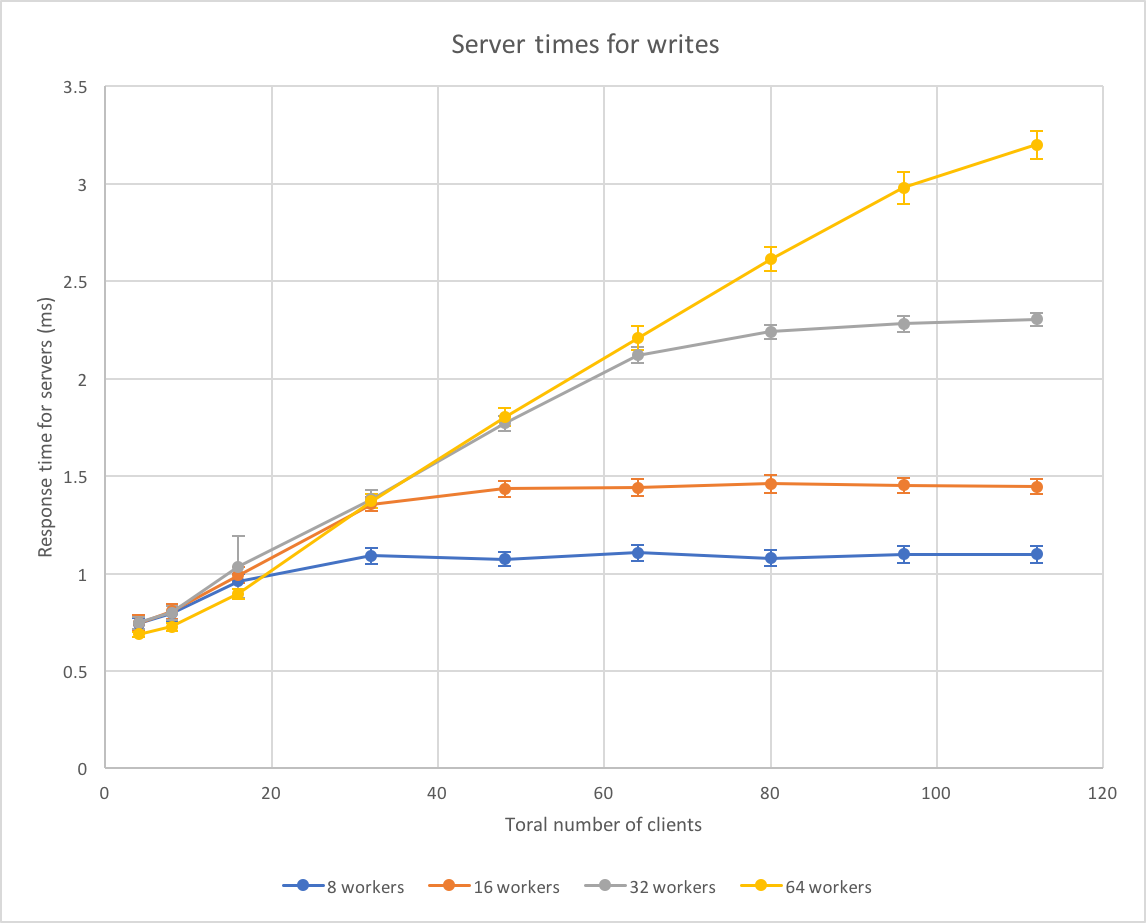
\includegraphics[width=\textwidth]{processing/graphics/bench_1mw_st_writes.png}
        \caption{Server time (time in network + time in server) for writes}
        \label{png::bench_1mw_st_writes}
    \end{minipage}
    \qquad
    \begin{minipage}[b]{.45\textwidth}
        \centering
        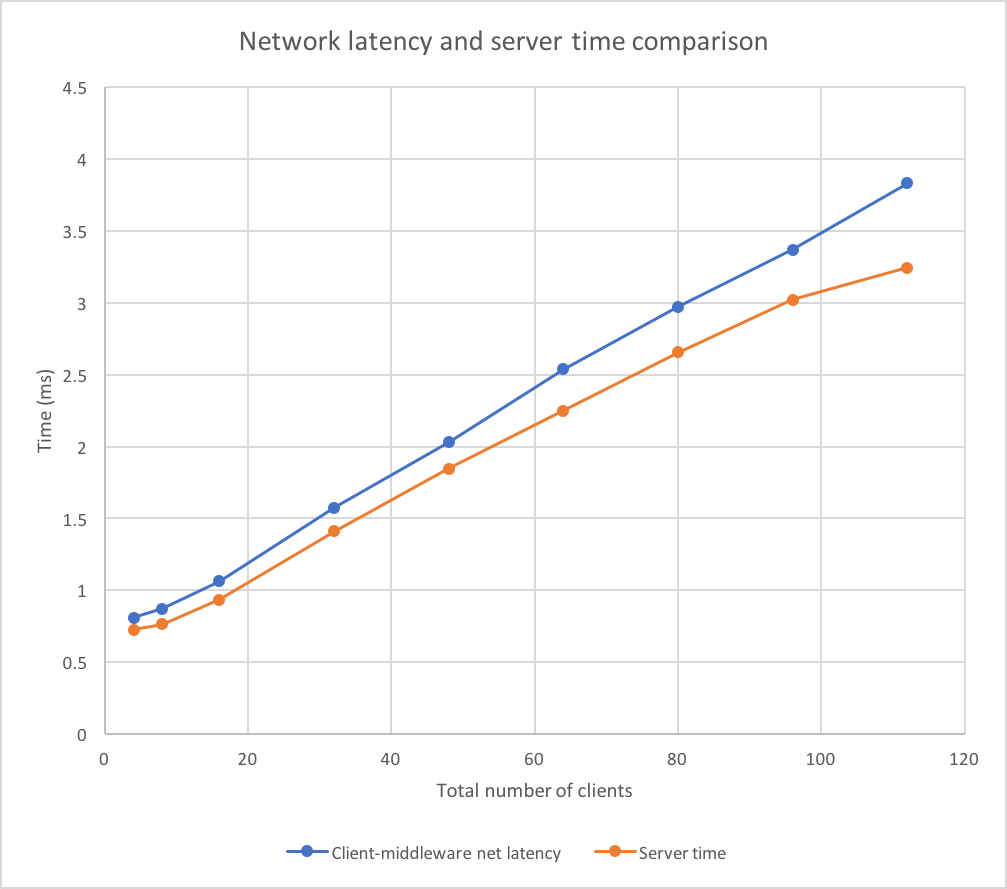
\includegraphics[width=\textwidth]{processing/graphics/bench_1mw_netlat_st_64writes.png}
        \caption{Network latency and server time for writes with 64 workers}
        \label{png::bench_1mw_netlat_st_64writes}
    \end{minipage}
\end{figure}



\subsection{Two middlewares}
In this subsection, two middleware machines are used. Each is connected to the same memcached server and a single load generating virtual machine hosts clients. Two instances of memtier, each running on a single thread, are connected to the two middlewares and the client count per thread is increased to study its impact on the behaviour of the system.

\subsubsection{Reads}
Figures \ref{png::bench_2mw_through-clients_reads} and \ref{png::bench_2mw_latency-clients_reads} show the throughput and response time as a function of client count for reads. Figure \ref{png::bench_2mw_through-clients_reads} shows the total throughput across both middlewares. Once again, data was evicted while the experiment was running. This causes throughput with 64 workers to increase above levels with other configurations. This is again due to the fact that the network is a bottlenecks for 8, 16, and 32 workers. The server cannot upload data fast enough to handle more requests. However, as data gets evicted, requests require less data to be uploaded by the server (due to empty responses), hence allowing more requests to be performed per second. Average hit to request ratio drops from 79.6\% to 8.7\%\footnote{\mintinline{shell}{processing/final/benchmark_2mw/benchmark_2mw.xlsx}} between 16 and 24 client runs with 64 workers. This results in a drop from 11.6MB to 2.6MB\footnote{\mintinline{shell}{processing/final/benchmark_2mw/dstat.csv}} of data per second uploaded by the server. Therefore, higher throughputs are possible.

\begin{figure}[!h]
    \centering
    \begin{minipage}[b]{.45\textwidth}
        \centering
        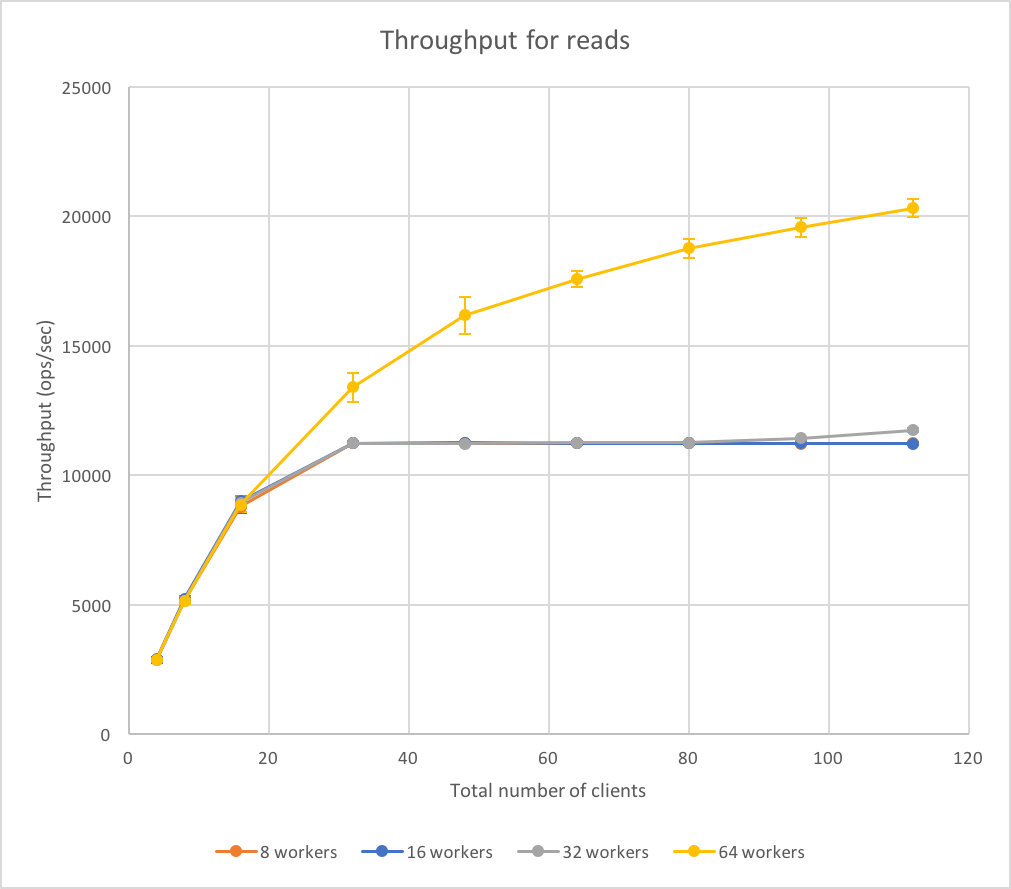
\includegraphics[width=\textwidth]{processing/graphics/bench_2mw_through-clients_reads.png}
        \caption{Throughput as a function of clients for reads}
        \label{png::bench_2mw_through-clients_reads}
    \end{minipage}
    \qquad
    \begin{minipage}[b]{.45\textwidth}
        \centering
        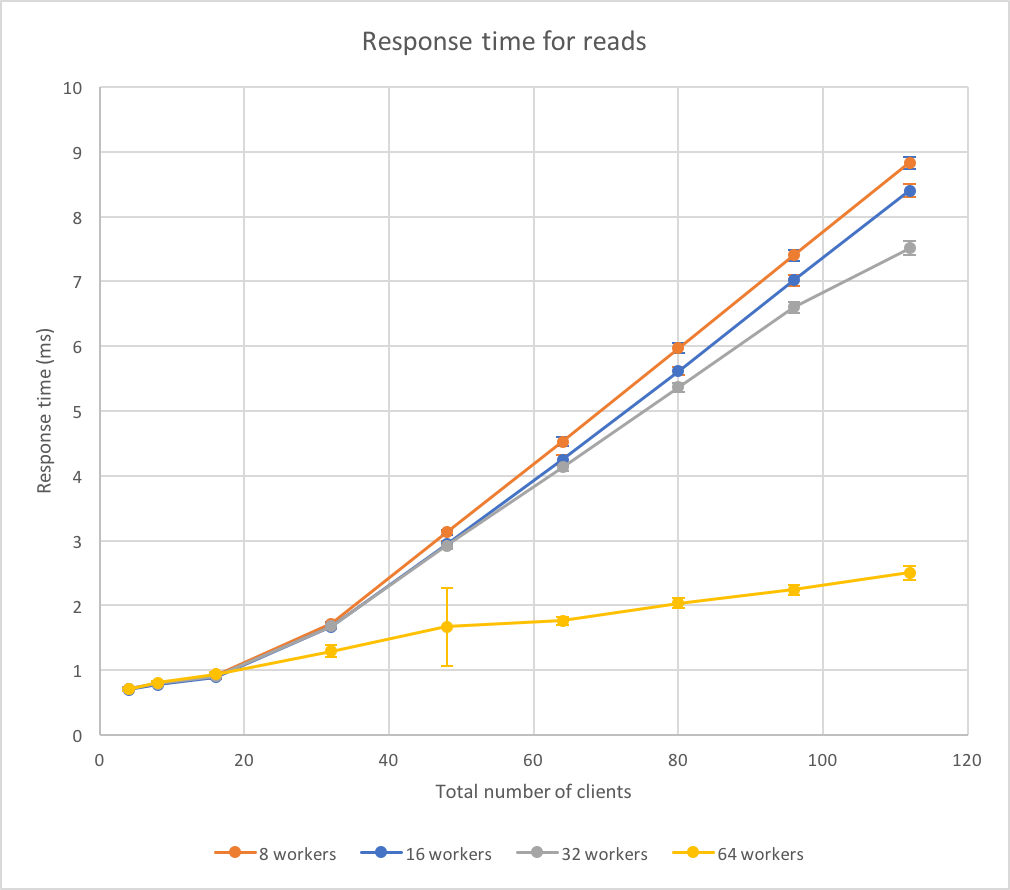
\includegraphics[width=\textwidth]{processing/graphics/bench_2mw_latency-clients_reads.png}
        \caption{Response time as a function of clients for reads}
        \label{png::bench_2mw_latency-clients_reads}
    \end{minipage}
\end{figure}

\subsubsection{Writes}
Figure \ref{png::bench_2mw_through-clients_writes} clearly has a dent with 16 workers. This is caused by a sudden increase in network latencies between the middleware and the memcached server. When testing with 16 workers, the last repetition with 32 clients per threads and the first repetition with 40 clients per thread experienced server times more than 2 times higher than normal\footnote{\mintinline{shell}{processing/processed/benchmark_2mw/ratio_1:0/sharded_false/workers_16/clients_32/mws.csv}}. The standard deviation in throughput and response time between repetitions hence increased thirtyfold between 24 and 32 clients\footnote{\mintinline{shell}{processing/final/benchmark_2mw/data.csv}}. It actually reached normal levels again only when testing with 56 clients per thread.

The increase in network latencies between middlewares and server is likely caused by a short burst in network traffic on Microsoft Azure resulting in higher network latencies between middlewares and server. Hence processing requests takes more time resulting in lower throughput and higher response times.

\begin{figure}[!h]
    \centering
    \begin{minipage}[b]{.45\textwidth}
        \centering
        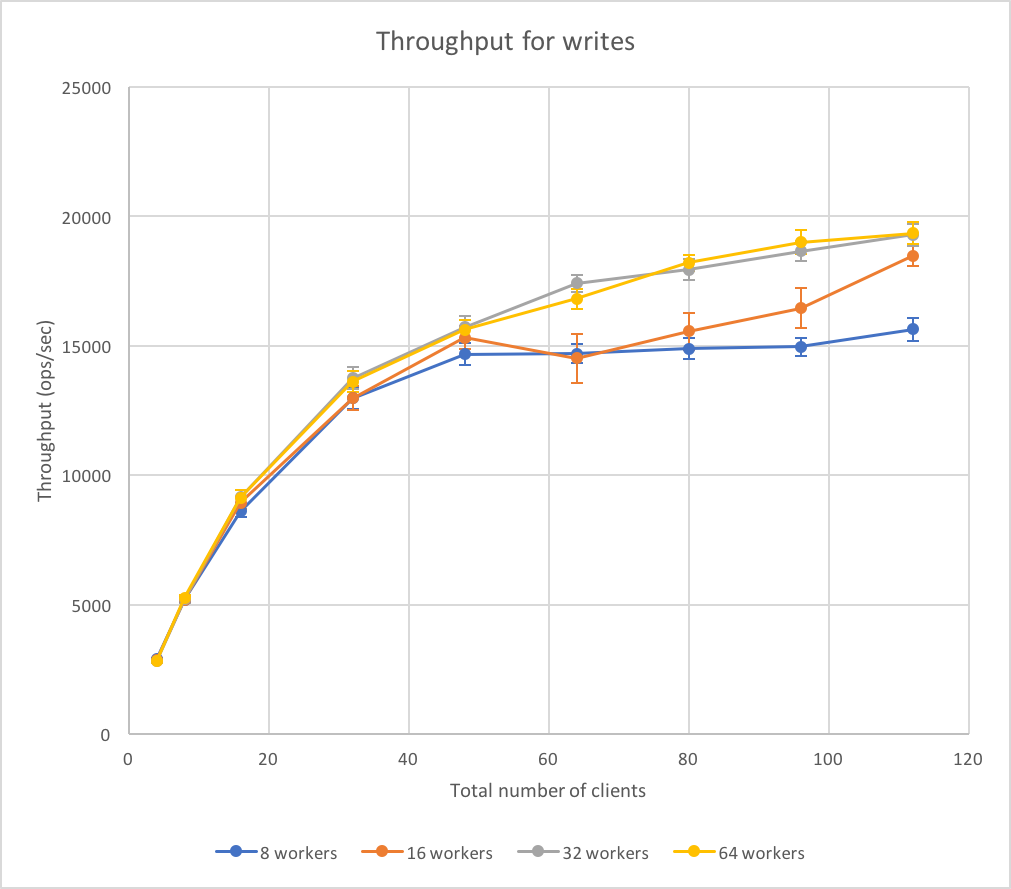
\includegraphics[width=\textwidth]{processing/graphics/bench_2mw_through-clients_writes.png}
        \caption{Throughput as a function of clients for writes}
        \label{png::bench_2mw_through-clients_writes}
    \end{minipage}
    \qquad
    \begin{minipage}[b]{.45\textwidth}
        \centering
        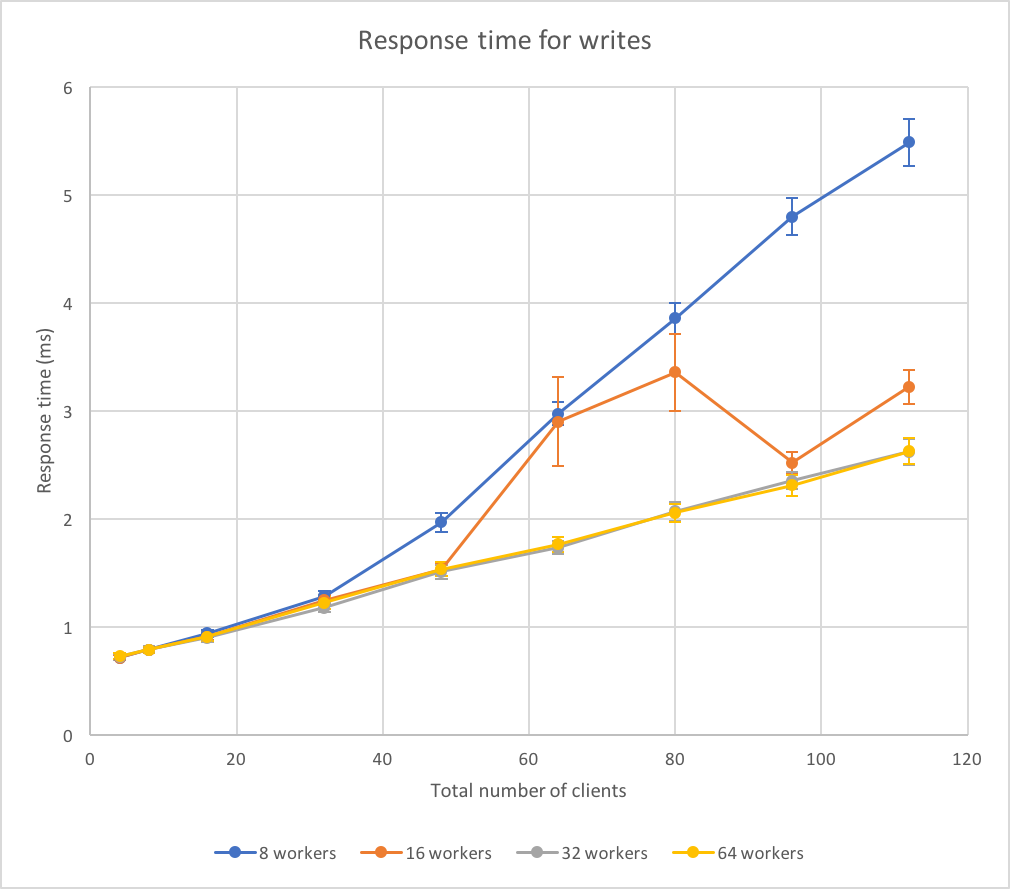
\includegraphics[width=\textwidth]{processing/graphics/bench_2mw_latency-clients_writes.png}
        \caption{Response time as a function of clients for writes}
        \label{png::bench_2mw_latency-clients_writes}
    \end{minipage}
\end{figure}

With these configurations, the bottleneck remains the server time. The queues in the middlewares are nearly empty potentially indicating that the net-thread cannot read the requests fast enough compared to the workers processing them. However, as the maximum of total clients is 112 (56 per middleware), it makes sense for the queues to be empty as the middleware uses more workers than the number requests it can receive at any one time.\\
Figure \ref{png::bench_2mw_netlat_writes} shows the difference in response time measured by the client and the middlewares. The dent for 16 workers is due to the fact that middleware 2 had very low server times at 96 clients\footnote{\mintinline{shell}{processing/processed/benchmark_2mw/ratio_1:0/sharded_false/workers_16/clients_48/mws.csv}}. This lead to reduced response times for said middleware, decreasing the average response time of the middleware and increasing the difference in measured response times between client and middlewares.

In all cases (8, 16, 32 and 64 workers), the response time difference between client and middlewares increases steadily. This suggests that the net-thread cannot read the requests fast enough to put them on the queue, hence creating latencies between client and middlewares. The reason the increase is less significant for 8 clients is that response time increases much more than for 32 or 64 clients. Hence less requests are in the network between client and middlewares at any given time, thus making the net-thread reading less of a bottleneck.

\begin{figure}[!h]
    \centering
    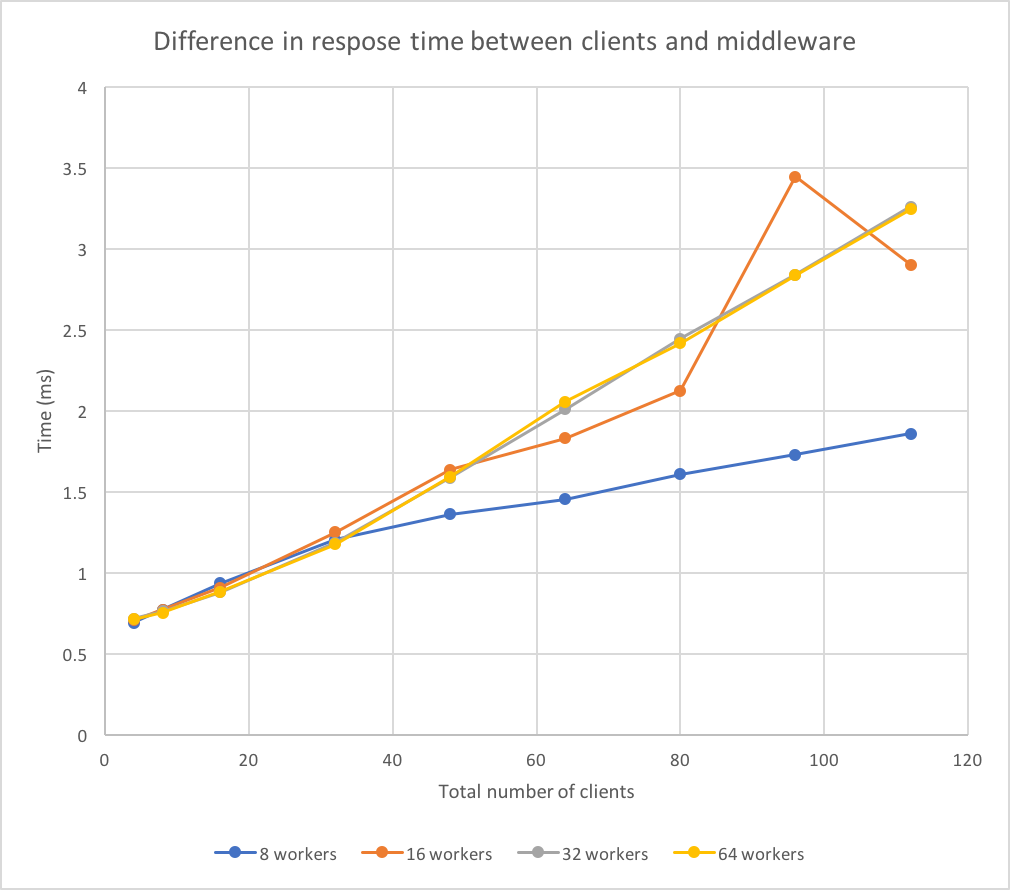
\includegraphics[width=.45\textwidth]{processing/graphics/bench_2mw_netlat_writes.png}
    \caption{Difference in response time between clients and middleware for writes}
    \label{png::bench_2mw_netlat_writes}
\end{figure}

\subsection{Summary}
Tables \ref{table::max_through_section_3_1mw} and \ref{table::max_through_section_3_2mw} show the maximum throughputs and the corresponding response times as measured by middlewares and the client machine. Note that for reads, the maximum throughputs were chosen irrespective of miss rates, hence the figures are much higher than could be expected with low miss rates. If hit rates were taken into account, the maximum throughput for reads would be comparable to the one in figure \ref{table::max_through_section_2} for a single server. This would be the case for both a system with a single middleware, and one with two middlewares. However, due to high miss rates, the server does not require much data to be sent back to the middleware(s). Therefore the network bandwidth no longer creates a bottleneck, allowing to obtain higher throughput.

Moreover, the system with two middlewares performs nearly twice as well as the system with a single one. Response times are reduced by about two milliseconds both as measured by middlewares and by clients. Average time spent in queue is also reduced considerably. This directly follows from the fact that less requests have to be handled \textit{per middleware} in a system with more middlewares.


\begin{table}[!h]
    \centering
    \begin{tabular}{|l|p{2cm}|p{2cm}|p{2cm}|p{2cm}|}
        \hline                                & Throughput & Response time & Average time in queue & Miss rate \\
        \hline Reads: Measured on middleware  &     14 162 &          4.54 &                  1.21 &     100\% \\
        \hline Reads: Measured on clients     &     14 049 &          7.98 & n/a                   &     100\% \\
        \hline Writes: Measured on middleware &     13 343 &          4.66 &                  1.41 & n/a       \\
        \hline Writes: Measured on clients    &     13 208 &          8.49 & n/a                   & n/a       \\
        \hline
    \end{tabular}
    \caption{Maximum throughput for one middleware}
    \label{table::max_through_section_3_1mw}
\end{table}

\begin{table}[!h]
    \centering
    \begin{tabular}{|l|p{2cm}|p{2cm}|p{2cm}|p{2cm}|}
        \hline                                & Throughput & Response time & Average time in queue & Miss rate \\
        \hline Reads: Measured on middleware  &     20 303 &          2.50 &                  0.47 &     100\% \\
        \hline Reads: Measured on clients     &     20 113 &          5.60 & n/a                   &     100\% \\
        \hline Writes: Measured on middleware &     19 349 &          2.63 &                  0.46 & n/a       \\
        \hline Writes: Measured on clients    &     19 205 &          5.87 & n/a                   & n/a       \\
        \hline
    \end{tabular}
    \caption{Maximum throughput for two middlewares}
    \label{table::max_through_section_3_2mw}
\end{table}

\newpage

\section{Throughput of writes \label{section::queue_model}}
During this experiment, three load generating virtual machines, running two instances of memtier each, are connected to two middlewares. Each instance of memtier runs on a single thread. The two middlewares are hosted on different virtual machines and are connected to three backend memcached servers.

As the title indicates, the experiment is run on write-only workloads with a range of different client numbers. Moreover, the number of worker threads is changed in the middlewares, same as in the last section.

As shown in figure \ref{png::throughput_writes_through-clients}, each increase in workers increases the overall performance of the system. The middlewares already saturate at 24 clients when running with 8 workers. This follows from the time taken for servers to respond to the middlewares. Note that the base time spent waiting for servers is much higher when using three backend servers compared to a single memcached server. This is caused by the fact that if one of the three servers is very slow (due to network latencies or CPU bounds), the worker is idle waiting for a response. Moreover, much more data has to be sent over the network since \textit{all} data from \mintinline{java}{set} requests is sent to all servers (not just parts such as in sharded \mintinline{java}{mutliget} requests). Hence, it requires the middlewares to send exactly three times as much data as with a single server. This results in longer response times and, by operational laws, in lower throughput.

\begin{figure}[!h]
    \centering
    \begin{minipage}[b]{.45\textwidth}
        \centering
        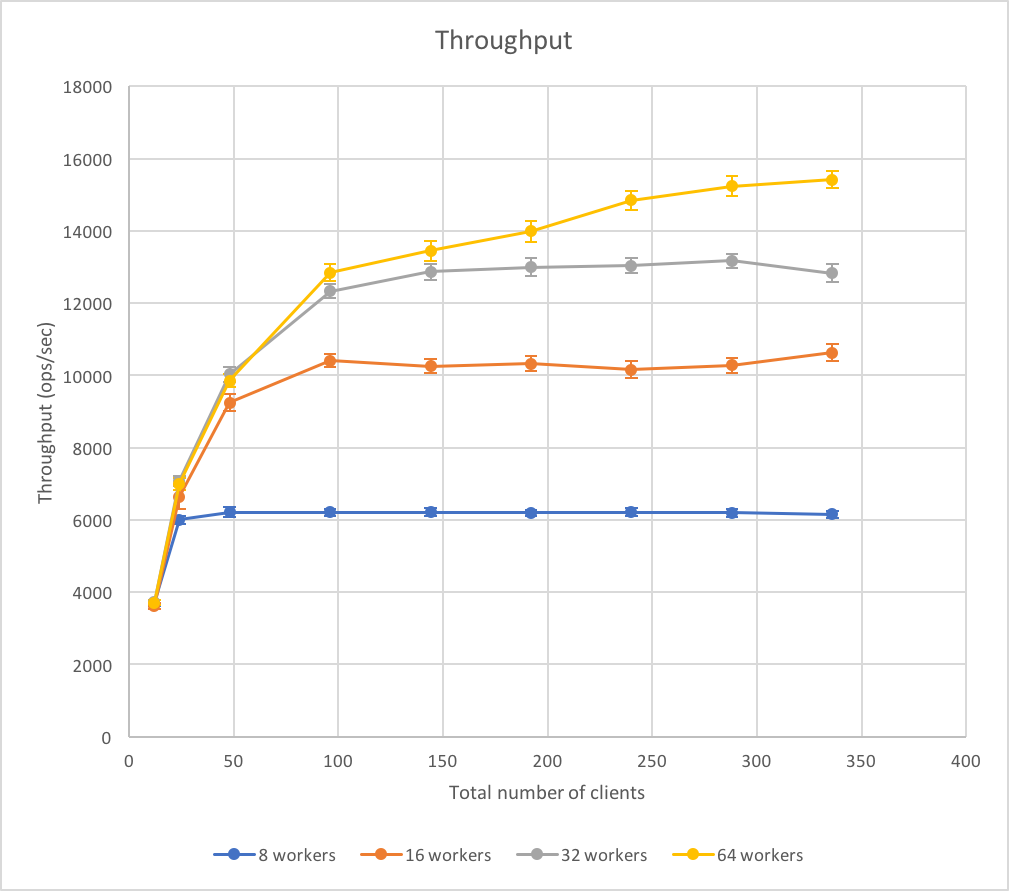
\includegraphics[width=\textwidth]{processing/graphics/throughput_writes_through-clients.png}
        \caption{Throughput as a function of clients}
        \label{png::throughput_writes_through-clients}
    \end{minipage}
    \qquad
    \begin{minipage}[b]{.45\textwidth}
        \centering
        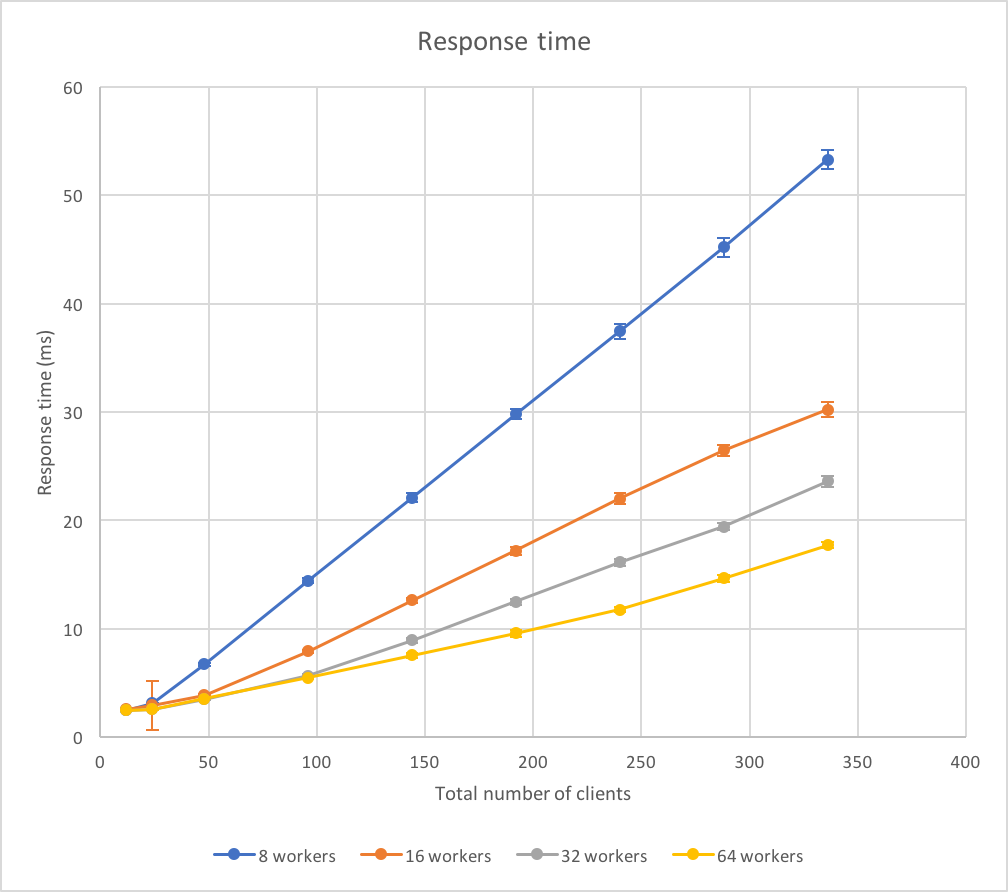
\includegraphics[width=\textwidth]{processing/graphics/throughput_writes_latency-clients.png}
        \caption{Response time as a function of clients}
        \label{png::throughput_writes_latency-clients}
    \end{minipage}
\end{figure}

Note that the drop in throughput compared to single server systems is very significant. In figure \ref{png::bench_2mw_through-clients_writes}, one can see throughput levels above 10 thousand requests per second. In the current case, 24 total clients results in barely over 6 thousand requests per second (figure \ref{png::throughput_writes_through-clients}). When comparing the time spend processing a request for both these system setups, one can see that the actual time spent processing (without time spent waiting for servers) is about the same at 0.03 milliseconds\footnote{\mintinline{shell}{processing/final/*/data.csv}}. However, the time spent waiting for servers changes considerably. With three servers, this is more constant as clients increase, only ranging from 2.38 to 2.55 milliseconds over the entire range of clients\footnote{\mintinline{shell}{processing/final/throughput_writes/data.csv}}. With a single server, the server time is less constant but much lower, increasing from 0.63 milliseconds for 4 clients to 1.41 milliseconds for 112 clients\footnote{\mintinline{shell}{processing/final/benchmark_2mw/data.csv}}. This stability in server time is only present for low worker count though. When running the middlewares with more workers, server times increase with client count as seen in figure \ref{png::throughput_writes_st}.

This general offset in server times when using three backend servers results in earlier saturation of the middlewares. Taking the configuration with 8 workers as an example once more, the system with a single memcached server saturates at 48 total clients (24 per middleware) as seen in figure \ref{png::bench_2mw_through-clients_writes}. In the case considered during this experiment, the system already saturates at 24 total clients (12 per middleware) as seen in figure \ref{png::throughput_writes_through-clients}.

For all worker configurations, the bottleneck is the service time of the servers. Moreover, due to the increase in server time, doubling the number of workers does not quite double the throughput at saturation level. However, note that in the case of switching from 8 workers to 16, the server time does not increase considerably, hence allowing for nearly twice the throughput at saturated levels (from about 6 thousand to about 10 thousand requests per second).

Figure \ref{png::throughput_writes_ql} shows how queue length varies with increases in client counts. On this graph, one can distinctly see how an increase in the number of clients on a saturated system simply increases the queue length linearly. For 8 workers, this happens beyond 24 clients; for 16 workers, beyond 48 clients; for 32 workers, beyond 96 clients; and for 64 workers at around 192 clients.

\begin{figure}[!h]
    \centering
    \begin{minipage}[b]{.45\textwidth}
        \centering
        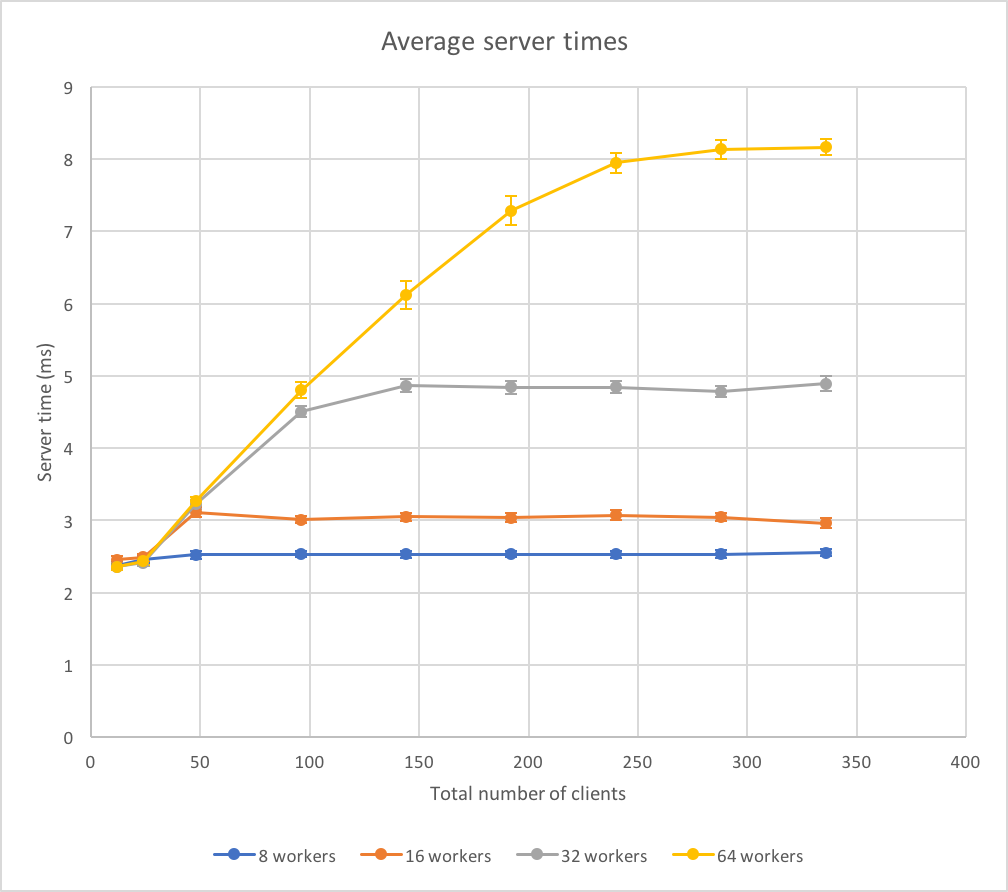
\includegraphics[width=\textwidth]{processing/graphics/throughput_writes_st.png}
        \caption{Average server times as a function of total number of clients}
        \label{png::throughput_writes_st}
    \end{minipage}
    \qquad
    \begin{minipage}[b]{.45\textwidth}
        \centering
        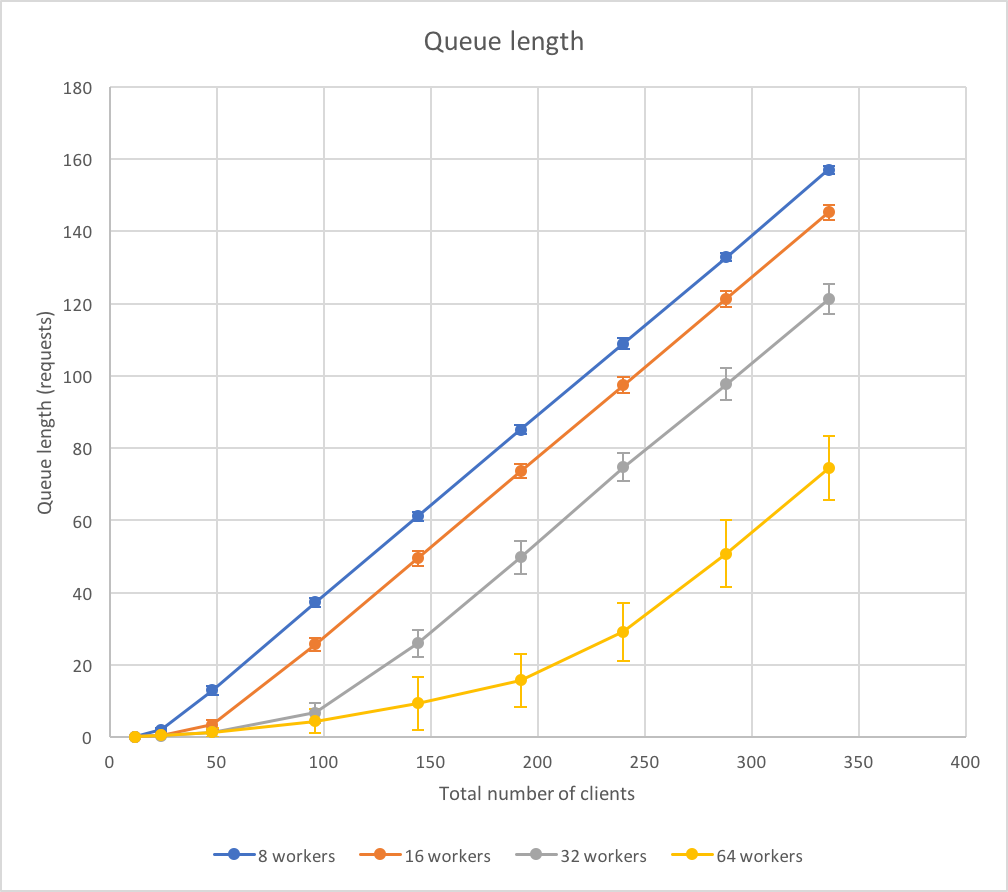
\includegraphics[width=\textwidth]{processing/graphics/throughput_writes_ql.png}
        \caption{Queue length as a function of total number of clients}
        \label{png::throughput_writes_ql}
    \end{minipage}
\end{figure}

Table \ref{table::max_through_section_4} shows maximum throughput as measured by middleware and clients as well as more information at that level of throughput. Note that for the throughput derived from the middleware response time, the following formula is used:
$$
X = \frac{N}{R + Z}
$$
The think time used ($Z$) is 0 as technically it would be equal to the time taken to send a response back to the client and the client sending a request back to the middleware. However, this would mean that $R + Z$, with $R$ being the response time measured by the middleware, is equal to the response time measured by the client. As this obviously follows operational laws, it would be redundant to compute this.

\begin{table}[!h]
    \centering
    \begin{tabular}{|l|p{1.5cm}|p{1.5cm}|p{1.5cm}|p{1.5cm}|}
        \hline                                            &   WT=8 &   WT=16 &   WT=32 &   WT=64 \\
        \hline Throughput (Middleware)                    &   6218 &  10 624 &  13 175 &  15 421 \\
        \hline Throughput (Derived from MW response time) &   6412 &  11 115 &  14 814 &  18 971 \\
        \hline Throughput (Client)                        &   6164 &  10 529 &  13 060 &  15 261 \\
        \hline Average time in queue                      &  34.88 &   27.24 &   14.62 &    9.50 \\
        \hline Average length of queue                    &  108.9 &   145.3 &    97.7 &    74.5 \\
        \hline Average time waiting for memcached         &   2.53 &    2.96 &    4.78 &    8.17 \\
        \hline
    \end{tabular}
    \caption{Maximum throughput for the full system}
    \label{table::max_through_section_4}
\end{table}

The figures displayed in table \ref{table::max_through_section_4} clearly show that 64 workers provide the highest throughput. Moreover, the gap between measured throughputs and throughputs computed with the interactive law increases with the number of workers. This is caused by the increase in difference between the response time measured by clients and the response time measured by the middlewares. That difference increases due to the fact that the net-thread has less available resources to read from the network as more worker threads read and write from network, hence creating a queue in the socket server. However, this is not a bottleneck as average queue lengths are still quite high. This would only become a problem if workers were able to process requests faster than the net-thread can read requests from the socket. However, this is by far not the case due to the time spent waiting for server responses.

\newpage

\section{Gets and Multigets}
In this section, three load generating client machines and three servers are used. Each load generating virtual machine runs two instances of memtier on a single thread with two clients each, and connected to one of two middlewares. Between repetitions, the number of keys requested by \mintinline{java}{multigets} is increased and tested on middleware configurations with both sharded and non-sharded reads. All middleware configurations use 64 clients.

Note that in order to correctly measure response times for \mintinline{java}{multigets}, the load used to portrait the data used below is read-only. Default load was used to check for behavioural changes in the middleware for mixed loads. However, the histograms acquired from the clients showed that the handling of \mintinline{java}{get} and \mintinline{java}{multiget} requests was unaffected by a mixed load. Therefore, as the middleware only outputs a single aggregate histogram for all types of requests, a read-only load is used in the analysis.

All standard deviations used for percentile information are computed as the deviation of all percentile measurements. Hence an average is taken across all repetitions, memtier machines, and memtier instances on each machine, and the standard deviation of these (18) measurements is used in the graphs for this section. Therefore, the error bars represent both variations between repetitions and variations across memtier instances.

Moreover, note that the actual sizes of the \mintinline{java}{multigets} is equivalent to their maximum size as the ratio was intentionally modified during the testing to ensure consistency. Therefore, from this point onwards, maximum key size will be equivalent to average \mintinline{java}{multiget} size.

\subsection{Sharded case}
Figures \ref{png::get_and_multigets_latency-keylen_sharded} shows the average response time as measured by clients and response times for 25\textsuperscript{th}, 50\textsuperscript{th}, 75\textsuperscript{th}, 90\textsuperscript{th} and 99\textsuperscript{th} percentiles.

\begin{figure}[!h]
    \centering
    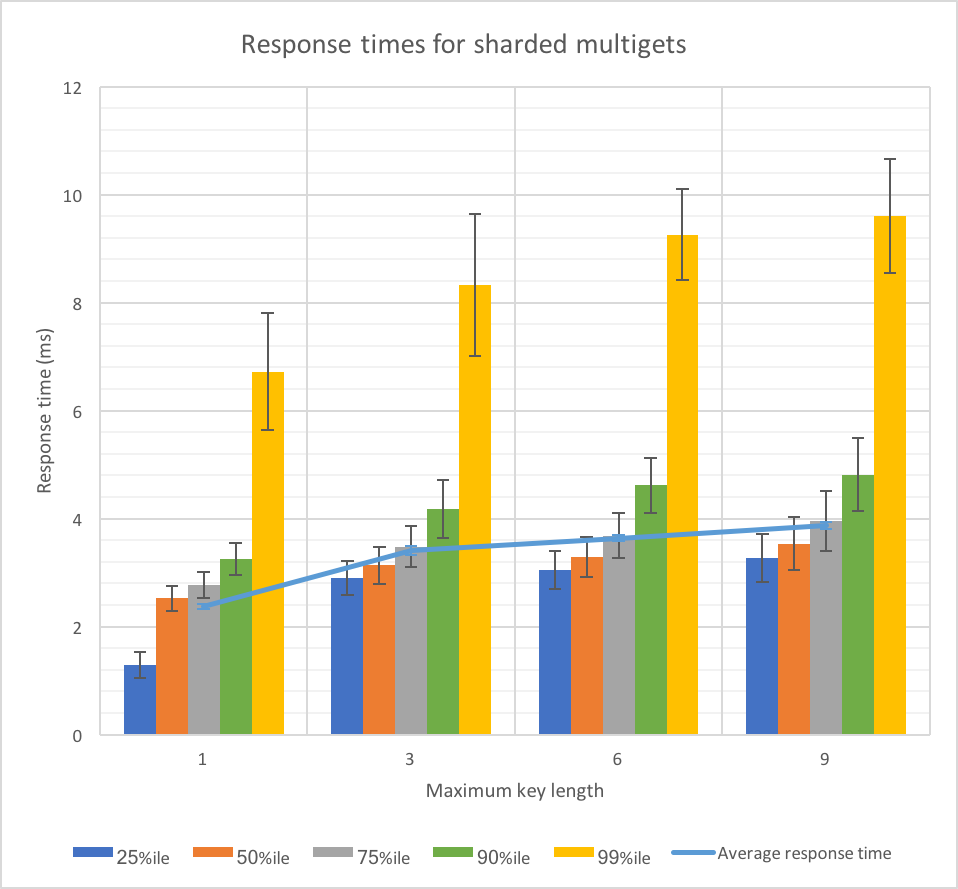
\includegraphics[width=0.6\textwidth]{processing/graphics/get_and_multigets_latency-keylen_sharded.png}
    \caption{Response times for sharded \mintinline{java}{multigets}}
    \label{png::get_and_multigets_latency-keylen_sharded}
\end{figure}

First, consider that a sharded \mintinline{java}{get} with a single key is equivalent to a non-sharded \mintinline{java}{get} of a single key. Hence the first data points are not representative of ``typical sharded behaviour''. Second, note that on actual sharded requests, the average response time is comparable to the response time from the 75\textsuperscript{th} percentile. This indicates that the 25\% of requests with the highest response times actually have much larger response times than the average, therefore resulting in a mean well above the median (50\textsuperscript{th} percentile). The reason for this phenomenon is that using three servers increases the likelihood of one server being slower than average.  In order to have a small server time, all contacted servers need to have low individual server times. This of course is much less likely than at least one server having a relatively long response time. In the latter case, the worker processing the sharded \mintinline{java}{multiget} is required to wait for the response of that server, significantly impacting overall response time for the client.

\subsubsection{Explanation}
Having only twelve total clients ($2\times6$ instances of memtier) distributed over two middlewares running both with 64 worker threads implies that workers are never completely utilised. In fact, most workers are idle during this experiment as too few requests are sent to the middlewares to require the usage of all workers. This is quite inefficient as those workers require memory and can create an unnecessary overhead with such a small number of clients.

Server response time still represents nearly the entire processing time. As long as this does not decrease, no higher throughputs are possible with a constant number of clients. However, for \mintinline{java}{multigets} of size 9, increasing the clients is actually very unlikely to improve throughput as the average amount of data sent to the network per server (10MB per second\footnote{\mintinline{shell}{processing/final/get_and_multigets/dstat.csv}}) is already reaching the maximum bandwidth.

The general increasing trend in average response times measured by the clients is due to increased server times as the maximum key number increases. This follows as a \mintinline{java}{multiget} with twice the number of keys requires twice as much data to be sent over the network and, unless memcached optimises \mintinline{java}{multigets}, twice the compute power for memcached.

\subsection{Non-Sharded case}
In the non-sharded case, average response time is comparable to the 50\textsuperscript{th} percentile response time (as seen on figure \ref{png::get_and_multigets_latency-keylen_non-sharded}). This follows from the middlewares only contacting a single server for each request, hence the likelihood of a server behaving better is comparable to the likelihood to a server behaving worse. As the worker thread handling the request does not need to wait for additional servers, these two scenarios balance out resulting in a mean relatively close to the median. However, note that the overall spread of percentile response times is larger than the one measured in the sharded case. This implies that the spread of the response time distribution is relatively broad, even if the average is close to the median.

\begin{figure}[!h]
    \centering
    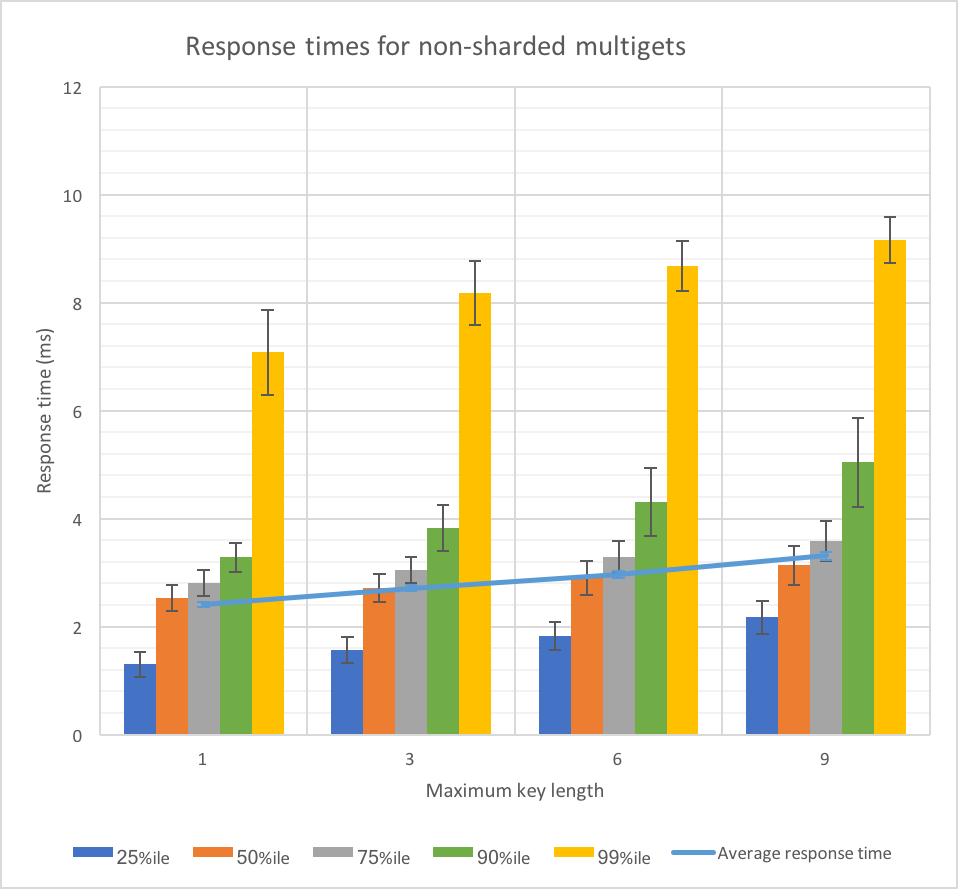
\includegraphics[width=0.6\textwidth]{processing/graphics/get_and_multigets_latency-keylen_non-sharded.png}
    \caption{Response times for non-sharded \mintinline{java}{multigets}}
    \label{png::get_and_multigets_latency-keylen_non-sharded}
\end{figure}

\subsubsection{Explanation}
As with the sharded case, the relatively low client count compared to the number of workers results in idle workers. Similarly to the sharded case, \mintinline{java}{multigets} of size 9 reach the network bandwidth with 11.5MB of data per second written to the network by servers. Hence increasing the client count would not result in higher throughputs.

The same increasing trend in average response times is visible for this configuration. This is caused for the same reasons as for sharded \mintinline{java}{multigets}.

\subsection{Histogram}
All histograms displayed in this section are the result of unweighted averages across all client instances / middleware hosts. Hence the histogram of response times given by some memtier instance has the same weight than any other memtier instance, irrespective of the actual throughput measured by said instance. This results in small inaccuracies in the data as memtier instances with smaller throughput should have a smaller impact on the histogram than other memtier instances.

\subsubsection{Sharded case}
Figure \ref{png::get_and_multigets_hist_sharded_clients} illustrates the response time histogram of sharded \mintinline{java}{multigets} as measured by the clients. Each bucket represents the percentage of total requests having a response time higher or equal to the bucket in question, yet lower than the next bucket. The first and last buckets represent the percentage of requests having lower and higher response times than the one indicated respectively.

As one can see, the vast majority of requests have a response time between 2.4 and 4.2 milliseconds. Moreover, the histogram shows a single peak in the distribution of response times. The reason for the very high percentage for the last bucket is only due to the grouping of all requests having response times higher than 6.9 milliseconds. The actual distribution decreases gradually until reaching zero.

\begin{figure}[!h]
    \centering
    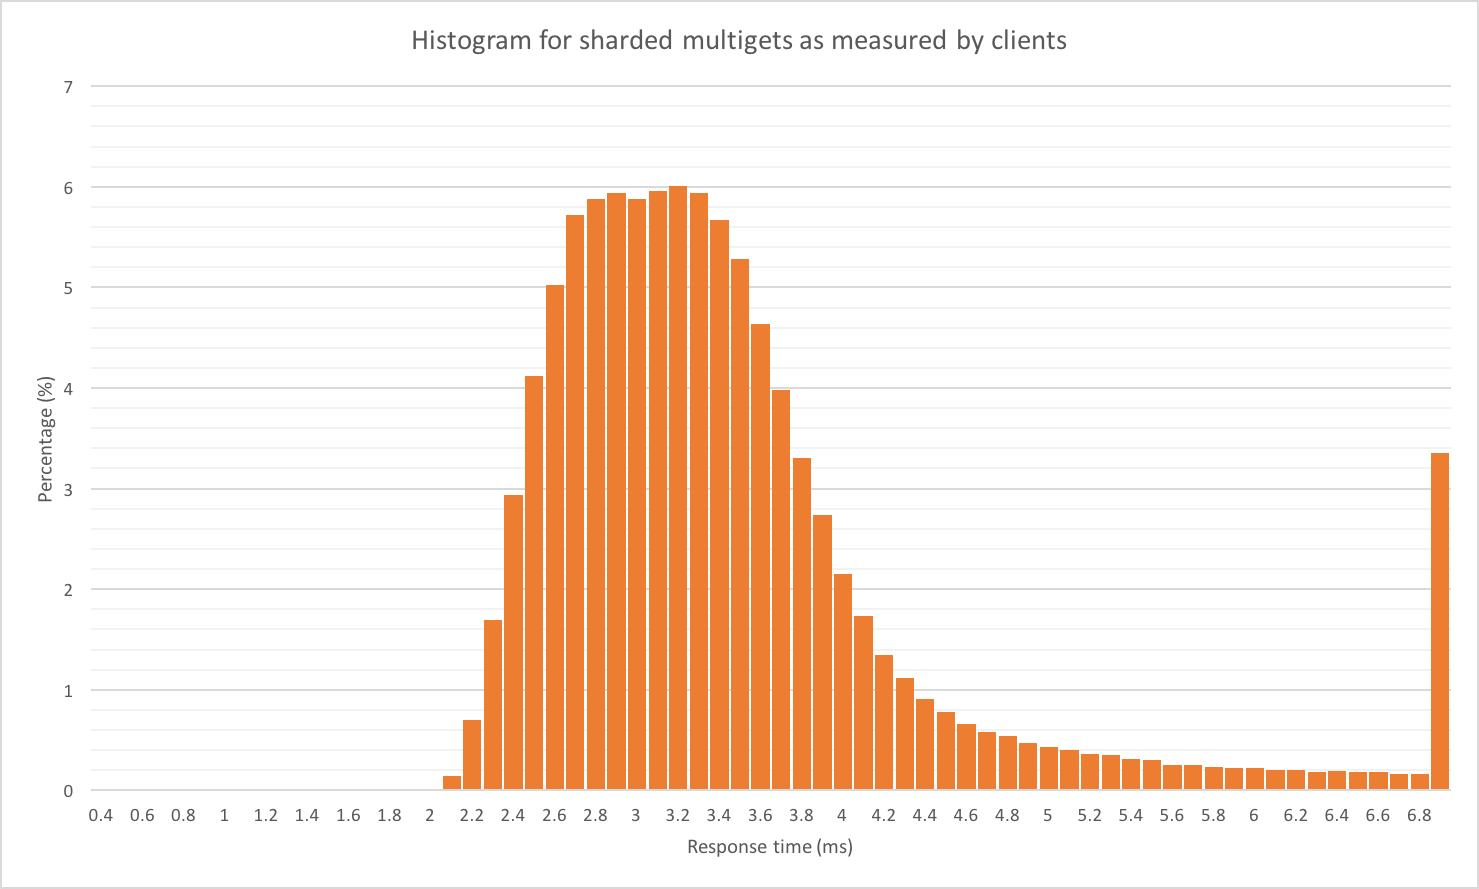
\includegraphics[width=0.7\textwidth]{processing/graphics/get_and_multigets_hist_sharded_clients.png}
    \caption{Histogram of response times for sharded \mintinline{java}{multigets} based on client data}
    \label{png::get_and_multigets_hist_sharded_clients}
\end{figure}

Figure \ref{png::get_and_multigets_hist_sharded_mws} represents the same data but measured on the middleware. As one can see, the overall response times are lower and more concentrated around the peak. The overall lower times are due to the fact that the time spent in network between clients and middlewares is not included in response time measurements for the middleware. The reason for more concentrated response times is the lack of network latency volatilities between clients and middlewares. These are random and add some spread to the response times observed by the clients.

\begin{figure}[!h]
    \centering
    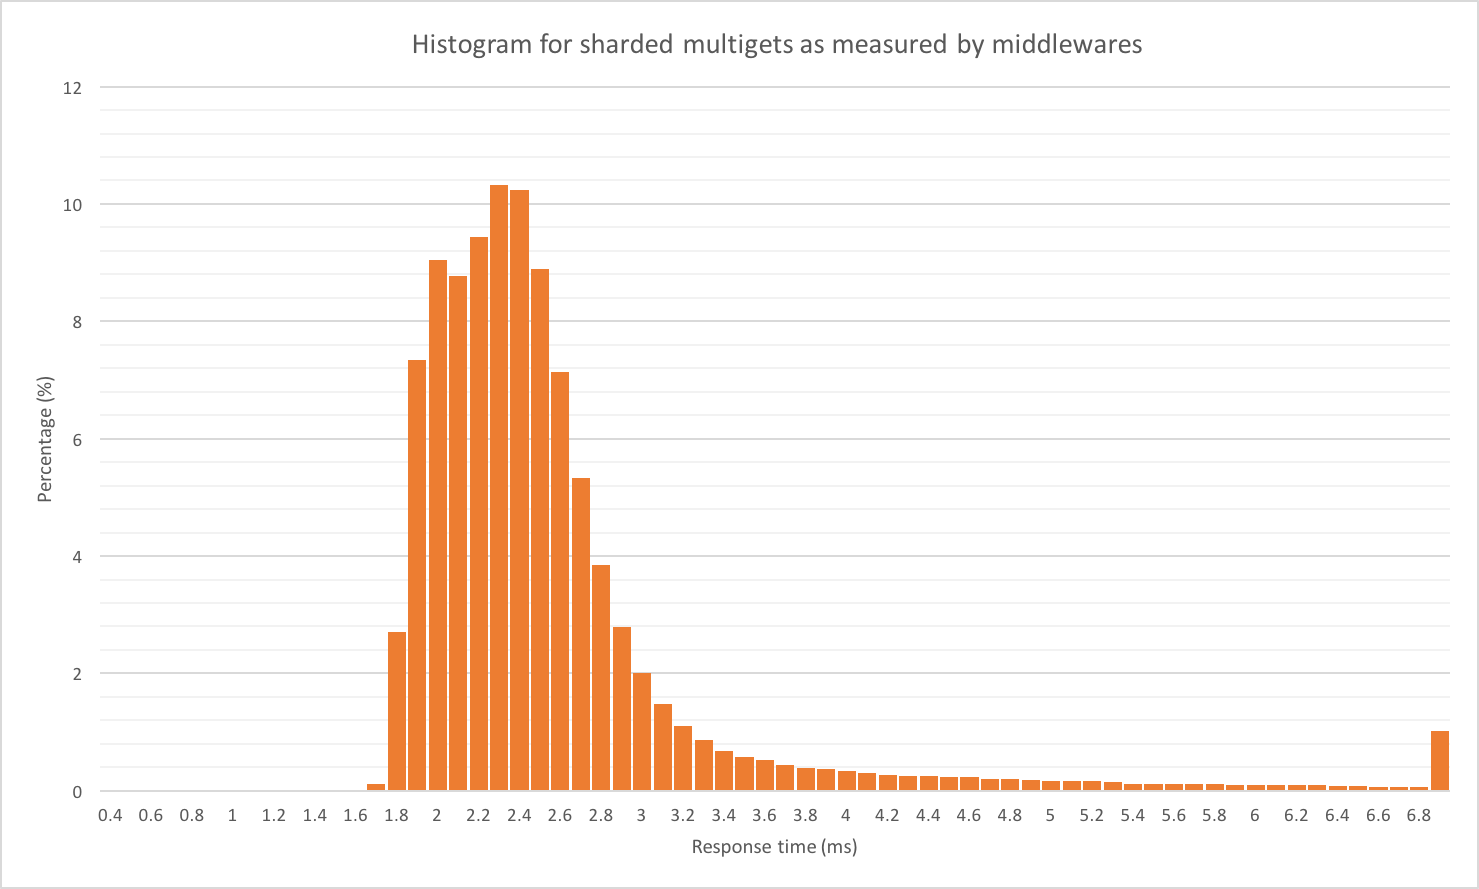
\includegraphics[width=0.7\textwidth]{processing/graphics/get_and_multigets_hist_sharded_mws.png}
    \caption{Histogram of response times for sharded \mintinline{java}{multigets} based on middleware data}
    \label{png::get_and_multigets_hist_sharded_mws}
\end{figure}

\subsubsection{Non-Sharded cases}
Figure \ref{png::get_and_multigets_hist_non-sharded_clients} shows the response times measured by clients for non-sharded \mintinline{java}{multigets}. As once can see, the overall spread of response times is much larger than for the sharded case. The vast majority of requests are amassed around two peaks. The second peak is comparable to the one seen in figure \ref{png::get_and_multigets_hist_sharded_clients} (if not as high) whereas the first peak has much lower response times. This is caused by network latencies being much lower for one server (namely ``\mintinline{java}{server1}''\footnote{\mintinline{shell}{logs/get_and_multigets(2017-11-18_13h10)/mw_._ping.log}}). In the sharded case, this did not impact service rates of the middleware as the middleware had to wait for all servers to respond. Hence the slowest servers (``\mintinline{java}{server2}'' and ``\mintinline{java}{server3}'') dictated the server time (here slow server means servers with high response times, even if due to network latencies). However, in the non-sharded case, about one third of all requests (due to load balancing) are sent to the server having lower network latencies, hence resulting in lower overall response times for this subset of requests. Because of this distribution of requests, one can also see that the first peak is smaller than the second one.

\begin{figure}[!h]
    \centering
    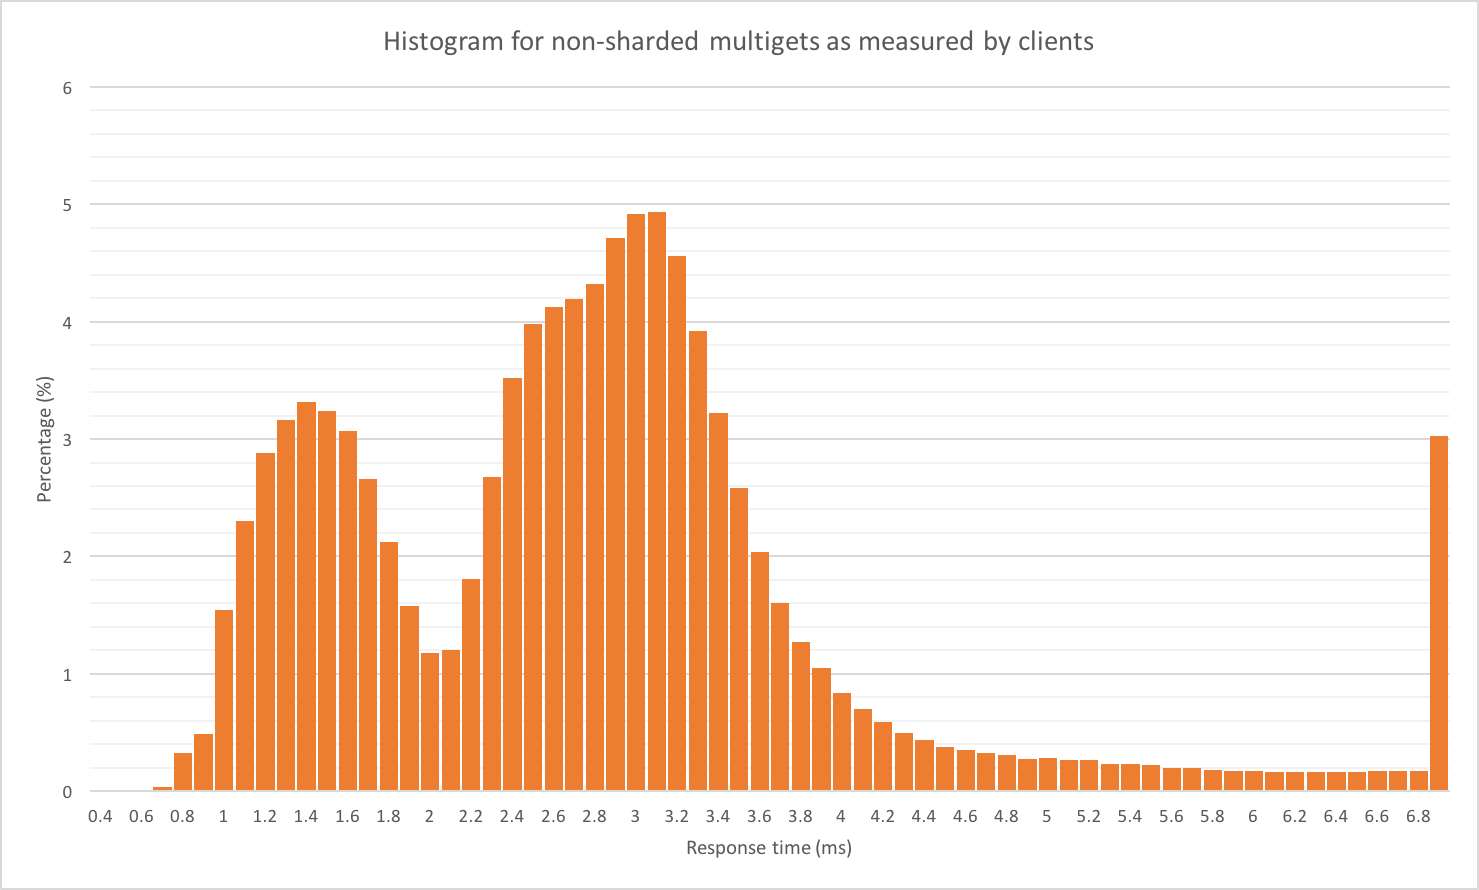
\includegraphics[width=0.7\textwidth]{processing/graphics/get_and_multigets_hist_non-sharded_clients.png}
    \caption{Histogram of response times for non-sharded \mintinline{java}{multigets} based on client data}
    \label{png::get_and_multigets_hist_non-sharded_clients}
\end{figure}

As seen in figure \ref{png::get_and_multigets_hist_non-sharded_mws}, the data collected on the middleware reflect the same as the clients. Moreover, the overall response times are again slightly lower than for clients and concentrated around the two peaks. This follows for the same reasons as for the sharded case.

\begin{figure}[!h]
    \centering
    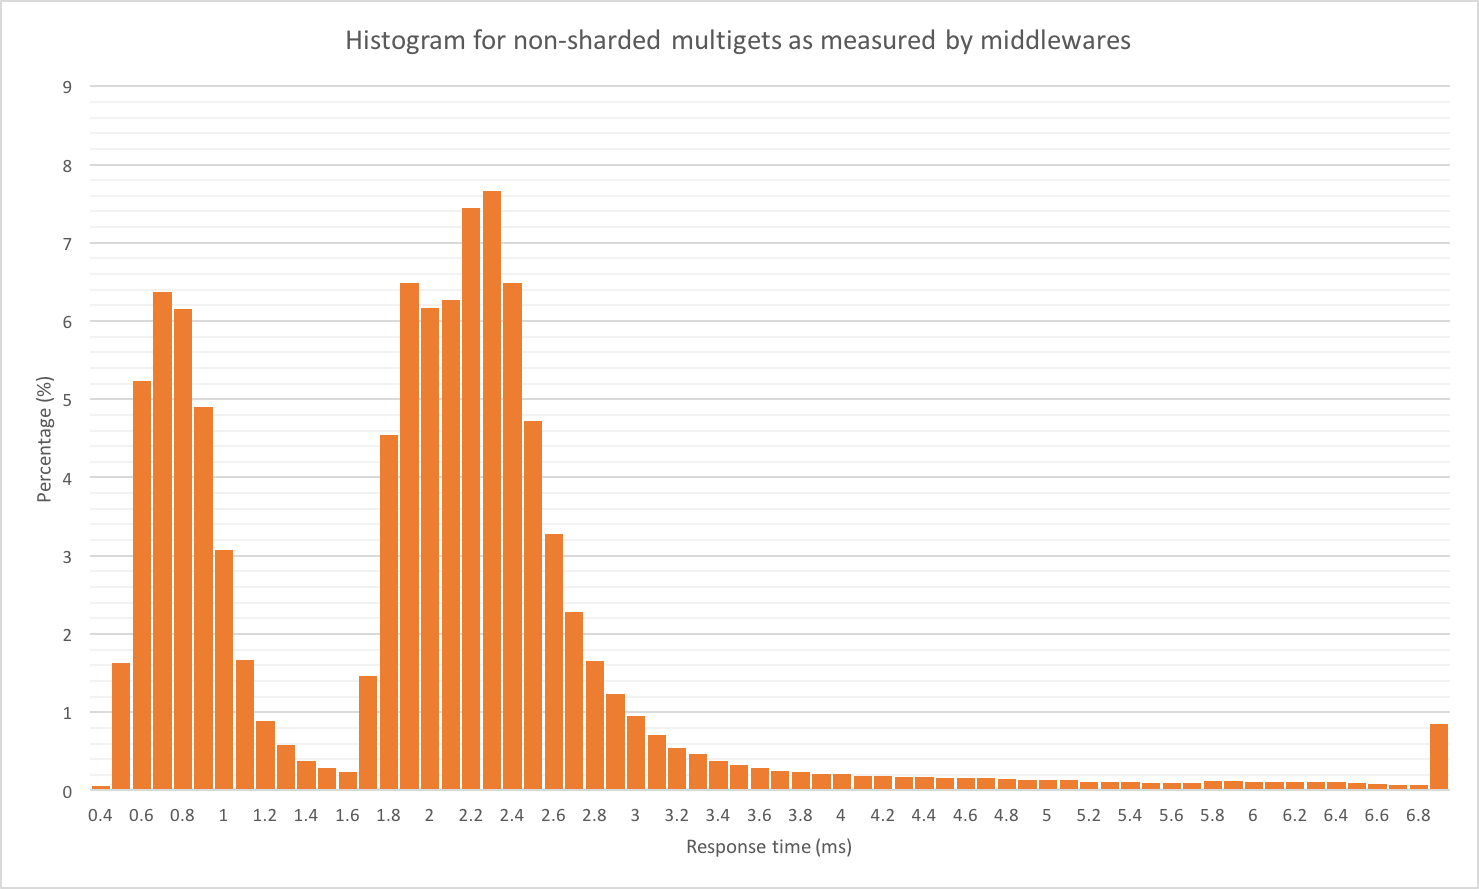
\includegraphics[width=0.7\textwidth]{processing/graphics/get_and_multigets_hist_non-sharded_mws.png}
    \caption{Histogram of response times for non-sharded \mintinline{java}{multigets} based on middleware data}
    \label{png::get_and_multigets_hist_non-sharded_mws}
\end{figure}

\subsection{Summary}
In general, non-sharded \mintinline{java}{multigets} are preferred over sharded ones. This is due to the fact that sharded requests cannot take advantage of the situation where a server or subset of servers behaves better than the rest. Therefore, non-sharded \mintinline{java}{multigets} have a lower average response time than sharded ones. However, due to the potentially large discrepancy between server behaviours, non-sharded requests are not very consistent in terms of response times. This is seen in figure \ref{png::get_and_multigets_latency-keylen_non-sharded}, where the difference in response times between 25\textsuperscript{th}, 50\textsuperscript{th}, and 75\textsuperscript{th} percentiles is much larger than in the sharded case. Nonetheless, as speed and throughput are usually the primary goals of such systems, non-sharded requests are superior.

\section{2K Analysis}
The experiments conducted in this section is are 6 different $2^k\cdot r$ experiments with three factors ($k = 3$) and three repetitions ($r = 3$). For three different types of workload (read-only, write-only, and read-write), the modified factors are:
\begin{enumerate}
    \item the number of servers used as backends (2 or 3), denoted $A$;
    \item the number of middlewares used (1 or 2), denoted $B$;
    \item the number of worker thread used per middleware (8 or 32), denoted $C$.
\end{enumerate}
Each of these configurations are then analysed for throughput and response time. Moreover, notice that all measurements will be taken from the middleware(s). This has the objective to reduce inaccuracies in variation measurements due to network latencies between clients and middlewares.

The following variables are defined:
\begin{align}
    x_A &=
    \begin{cases}
        -1 \quad &\text{if 2 servers are used}\\
        1 \quad &\text{if 3 servers are used}
    \end{cases}\label{eq::x_a}\\
    x_B &=
    \begin{cases}
        -1 \quad &\text{if 1 middleware is used}\\
        1 \quad &\text{if 2 middlewares are used}
    \end{cases}\label{eq::x_b}\\
    x_C &=
    \begin{cases}
        -1 \quad &\text{if 8 workers are used}\\
        1 \quad &\text{if 32 workers are used}
    \end{cases}\label{eq::x_c}
\end{align}

The model used is multiplicative as every middleware has a number of workers and each of these workers is connected to all servers. Therefore, the data in the following tables under the headings ``Repetitions'' is actually the \textbf{logarithm} of throughput or response time. All other computations within the tables is then based on that data.

\subsection{Read-only workload}
Table \ref{table::ro_2k_through} illustrates the impact on throughput of changing the factors. The last row in this table gives the portion of the variation affected by the change in the given factor.

From the last row in said table, one can see that the only factors affecting throughput are the number of middlewares and the number of workers. The number of workers has a slightly bigger impact, as the actual change in number of workers quadruples when going from 8 to 32 workers, whereas only doubles by adding a second middleware. However, note that the effect of increasing workers is only slightly better than the effect of adding a middleware. Therefore, it is preferred to increase from one middleware to two rather than doubling the number of workers on a single middleware.

All cross-effects between variables are insignificant, not even reaching one percent in any of the cases.


\afterpage{%
    \clearpage% Flush earlier floats (otherwise order might not be correct)
    \thispagestyle{fancy}%
    \begin{landscape}% Landscape page
        \centering

        \vspace*{1cm}

        \resizebox{0.75\paperheight}{!}{
            \begin{tabular}{|*{15}{r|}}
                \hline\multicolumn{8}{|c|}{\textbf{Configuration}} & \multicolumn{3}{|c|}{\textbf{Repetitions}} & \multicolumn{4}{|c|}{\textbf{Statistics}} \\
                \hline\multicolumn{1}{|c|}{$I$} & \multicolumn{1}{|c|}{$A$} & \multicolumn{1}{|c|}{$B$} & \multicolumn{1}{|c|}{$C$} & \multicolumn{1}{|c|}{$AB$} & \multicolumn{1}{|c|}{$AC$} & \multicolumn{1}{|c|}{$BC$} & \multicolumn{1}{|c|}{$ABC$} & \multicolumn{1}{|c|}{1} & \multicolumn{1}{|c|}{2} & \multicolumn{1}{|c|}{3} & \multicolumn{1}{|c|}{mean} & \multicolumn{1}{|c|}{error 1} & \multicolumn{1}{|c|}{error 2} & \multicolumn{1}{|c|}{error 3} \\
                \hline\hline 1 & 1 & 1 & 1 & 1 & 1 & 1 & 1 & 4.338152331 & 4.341791014 & 4.351575288 & 4.343839544 & -0.005687213 & -0.00204853 & 0.007735743 \\
                \hline 1 & 1 & 1 & -1 & 1 & -1 & -1 & -1 & 3.974227789 & 3.967104915 & 3.973830703 & 3.971721136 & 0.002506653 & -0.004616221 & 0.002109567 \\
                \hline 1 & 1 & -1 & 1 & -1 & 1 & -1 & -1 & 4.03632692 & 4.035952778 & 4.034917589 & 4.035732429 & 0.000594491 & 0.000220349 & -0.00081484 \\
                \hline 1 & 1 & -1 & -1 & -1 & -1 & 1 & 1 & 3.619358159 & 3.619262944 & 3.624463873 & 3.621028325 & -0.001670166 & -0.001765382 & 0.003435548 \\
                \hline 1 & -1 & 1 & 1 & -1 & -1 & 1 & -1 & 4.347825024 & 4.350403338 & 4.350422961 & 4.349550441 & -0.001725417 & 0.000852897 & 0.00087252 \\
                \hline 1 & -1 & 1 & -1 & -1 & 1 & -1 & 1 & 4.022168459 & 4.030861717 & 4.034256862 & 4.029095679 & -0.00692722 & 0.001766038 & 0.005161182 \\
                \hline 1 & -1 & -1 & 1 & 1 & -1 & -1 & 1 & 4.045849877 & 4.051759146 & 4.042921865 & 4.046843629 & -0.000993752 & 0.004915517 & -0.003921764 \\
                \hline 1 & -1 & -1 & -1 & 1 & 1 & 1 & -1 & 3.686242903 & 3.685602921 & 3.689396553 & 3.687080792 & -0.00083789 & -0.001477871 & 0.002315761 \\
                \hline\multicolumn{15}{|c|}{\textbf{Aggregates}} \\
                \hline 32.08489198 & -0.140249107 & 1.303521624 & 1.467040111 & 0.014078227 & 0.106604914 & -0.08189377 & -0.00327762 & \multicolumn{3}{|l|}{\textbf{Total}} & \multicolumn{2}{|r|}{} & \textbf{SST} & \textbf{SSE} \\
                \hline 4.010611497 & -0.017531138 & 0.162940203 & 0.183380014 & 0.001759778 & 0.013325614 & -0.010236721 & -0.000409702 & \multicolumn{3}{|l|}{\textbf{Total/8}} & \multicolumn{2}{|r|}{} & 1.458775161 & 0.000278188 \\
                \hline & 0.505641976 & 43.67967397 & 55.32569577 & 0.005094937 & 0.292144257 & 0.172402927 & 0.00027616 & \multicolumn{3}{|l|}{\textbf{Percentage impact}} & \multicolumn{4}{|l|}{} \\
                \hline
            \end{tabular}
        }
        \captionof{table}{Read-only 2\textsuperscript{k}r analysis for throughput}
        \label{table::ro_2k_through}

        \vspace{2cm}

        \resizebox{0.75\paperheight}{!}{
            \begin{tabular}{|*{15}{r|}}
                \hline\multicolumn{8}{|c|}{\textbf{Configuration}} & \multicolumn{3}{|c|}{\textbf{Repetitions}} & \multicolumn{4}{|c|}{\textbf{Statistics}} \\
                \hline\multicolumn{1}{|c|}{$I$} & \multicolumn{1}{|c|}{$A$} & \multicolumn{1}{|c|}{$B$} & \multicolumn{1}{|c|}{$C$} & \multicolumn{1}{|c|}{$AB$} & \multicolumn{1}{|c|}{$AC$} & \multicolumn{1}{|c|}{$BC$} & \multicolumn{1}{|c|}{$ABC$} & \multicolumn{1}{|c|}{1} & \multicolumn{1}{|c|}{2} & \multicolumn{1}{|c|}{3} & \multicolumn{1}{|c|}{mean} & \multicolumn{1}{|c|}{error 1} & \multicolumn{1}{|c|}{error 2} & \multicolumn{1}{|c|}{error 3} \\
                \hline\hline 1 & 1 & 1 & 1 & 1 & 1 & 1 & 1 & 0.826011299 & 0.82045359 & 0.805116722 & 0.81719387 & 0.008817429 & 0.00325972 & -0.012077148 \\
                \hline 1 & 1 & 1 & -1 & 1 & -1 & -1 & -1 & 1.287864319 & 1.29415737 & 1.287244059 & 1.28975525 & -0.001890931 & 0.004402121 & -0.00251119 \\
                \hline 1 & 1 & -1 & 1 & -1 & 1 & -1 & -1 & 1.187524257 & 1.188001791 & 1.187870768 & 1.187798939 & -0.000274682 & 0.000202853 & 7.18296E-05 \\
                \hline 1 & 1 & -1 & -1 & -1 & -1 & 1 & 1 & 1.648799585 & 1.649266261 & 1.644363093 & 1.647476313 & 0.001323272 & 0.001789948 & -0.00311322 \\
                \hline 1 & -1 & 1 & 1 & -1 & -1 & 1 & -1 & 0.806318625 & 0.820689889 & 0.808797077 & 0.811935197 & -0.005616572 & 0.008754692 & -0.00313812 \\
                \hline 1 & -1 & 1 & -1 & -1 & 1 & -1 & 1 & 1.236231432 & 1.227235028 & 1.223332742 & 1.228933067 & 0.007298365 & -0.001698039 & -0.005600325 \\
                \hline 1 & -1 & -1 & 1 & 1 & -1 & -1 & 1 & 1.171455198 & 1.164427122 & 1.173661728 & 1.169848016 & 0.001607182 & -0.005420894 & 0.003813712 \\
                \hline 1 & -1 & -1 & -1 & 1 & 1 & 1 & -1 & 1.579507473 & 1.581580792 & 1.577908109 & 1.579665458 & -0.000157985 & 0.001915334 & -0.001757349 \\
                \hline\multicolumn{15}{|c|}{\textbf{Aggregates}} \\
                \hline 9.73260611 & 0.151842633 & -1.436971342 & -1.759054066 & -0.019680922 & -0.105423442 & -0.020064433 & -0.005703578 & \multicolumn{3}{|l|}{\textbf{Total}} & \multicolumn{2}{|r|}{} & \textbf{SST} & \textbf{SSE} \\
                \hline 1.216575764 & 0.018980329 & -0.179621418 & -0.219881758 & -0.002460115 & -0.01317793 & -0.002508054 & -0.000712947 & \multicolumn{3}{|l|}{\textbf{Total/8}} & \multicolumn{2}{|r|}{} & 1.948343575 & 0.000537106 \\
                \hline & 0.443765132 & 39.74311818 & 59.55580511 & 0.007455154 & 0.213914441 & 0.007748533 & 0.000626124 & \multicolumn{3}{|l|}{\textbf{Percentage impact}} & \multicolumn{4}{|l|}{} \\
                \hline
            \end{tabular}
        }
        \captionof{table}{Read-only 2\textsuperscript{k}r analysis for response time}
        \label{table::ro_2k_latency}

    \end{landscape}
    \clearpage% Flush page
}

As expected, the results observed in table \ref{table::ro_2k_latency} show the same behaviour to the previous table mapped to response time. However, impacts have grown in importance. This entire shift in the significance of the factors is caused by the network latencies between middleware and clients not being taken into account. As a consequence, the response times used in table \ref{table::ro_2k_latency} are lower than the actual one. Therefore changes in response time caused by the modifications in the configuration feel more significant than when measured by the client.


\subsection{Write-only workload}
Table \ref{table::wo_2k_through} illustrates the effect of changes in the factors outlined in equation \ref{eq::x_a}, \ref{eq::x_b} and \ref{eq::x_c}. For write-only workloads, the effects observed are extremely similar to read-only workloads, both for throughput and response time.

\afterpage{%
    \clearpage% Flush earlier floats (otherwise order might not be correct)
    \thispagestyle{fancy}%
    \begin{landscape}% Landscape page
        \centering

        \vspace*{1cm}

        \resizebox{0.75\paperheight}{!}{
            \begin{tabular}{|*{15}{r|}}
                \hline\multicolumn{8}{|c|}{\textbf{Configuration}} & \multicolumn{3}{|c|}{\textbf{Repetitions}} & \multicolumn{4}{|c|}{\textbf{Statistics}} \\
                \hline\multicolumn{1}{|c|}{$I$} & \multicolumn{1}{|c|}{$A$} & \multicolumn{1}{|c|}{$B$} & \multicolumn{1}{|c|}{$C$} & \multicolumn{1}{|c|}{$AB$} & \multicolumn{1}{|c|}{$AC$} & \multicolumn{1}{|c|}{$BC$} & \multicolumn{1}{|c|}{$ABC$} & \multicolumn{1}{|c|}{1} & \multicolumn{1}{|c|}{2} & \multicolumn{1}{|c|}{3} & \multicolumn{1}{|c|}{mean} & \multicolumn{1}{|c|}{error 1} & \multicolumn{1}{|c|}{error 2} & \multicolumn{1}{|c|}{error 3} \\
                \hline\hline 1 & 1 & 1 & 1 & 1 & 1 & 1 & 1 & 4.100565245 & 4.108614911 & 4.109351976 & 4.106177377 & -0.005612133 & 0.002437533 & 0.003174599 \\
                \hline 1 & 1 & 1 & -1 & 1 & -1 & -1 & -1 & 3.784667209 & 3.788414095 & 3.78358828 & 3.785556528 & -0.000889319 & 0.002857567 & -0.001968248 \\
                \hline 1 & 1 & -1 & 1 & -1 & 1 & -1 & -1 & 3.80815187 & 3.801720053 & 3.808356164 & 3.806076029 & 0.002075841 & -0.004355976 & 0.002280135 \\
                \hline 1 & 1 & -1 & -1 & -1 & -1 & 1 & 1 & 3.423945917 & 3.418226692 & 3.415670165 & 3.419280925 & 0.004664992 & -0.001054232 & -0.003610759 \\
                \hline 1 & -1 & 1 & 1 & -1 & -1 & 1 & -1 & 4.162679013 & 4.161450361 & 4.165328921 & 4.163152765 & -0.000473751 & -0.001702404 & 0.002176156 \\
                \hline 1 & -1 & 1 & -1 & -1 & 1 & -1 & 1 & 3.802315251 & 3.798190388 & 3.795133258 & 3.798546299 & 0.003768952 & -0.000355911 & -0.003413041 \\
                \hline 1 & -1 & -1 & 1 & 1 & -1 & -1 & 1 & 3.858680034 & 3.88385654 & 3.883808304 & 3.875448293 & -0.016768259 & 0.008408247 & 0.008360011 \\
                \hline 1 & -1 & -1 & -1 & 1 & 1 & 1 & -1 & 3.448317831 & 3.445220719 & 3.450012261 & 3.44785027 & 0.000467561 & -0.002629552 & 0.002161991 \\
                \hline\multicolumn{15}{|c|}{\textbf{Aggregates}} \\
                \hline 30.40208849 & -0.167906768 & 1.304777452 & 1.499620442 & 0.02797645 & -0.084788535 & -0.129165811 & -0.003182698 & \multicolumn{3}{|l|}{\textbf{Total}} & \multicolumn{2}{|r|}{} & \textbf{SST} & \textbf{SSE} \\
                \hline 3.800261061 & -0.020988346 & 0.163097182 & 0.187452555 & 0.003497056 & -0.010598567 & -0.016145726 & -0.000397837 & \multicolumn{3}{|l|}{\textbf{Total/8}} & \multicolumn{2}{|r|}{} & 1.502153674 & 0.000592149 \\
                \hline & 0.703806555 & 42.50008412 & 56.14093056 & 0.019538991 & 0.179469712 & 0.416497172 & 0.000252876 & \multicolumn{3}{|l|}{\textbf{Percentage impact}} & \multicolumn{4}{|l|}{} \\
                \hline
            \end{tabular}
        }
        \captionof{table}{Write-only 2\textsuperscript{k}r analysis for throughput}
        \label{table::wo_2k_through}

        \vspace{2cm}

        \resizebox{0.75\paperheight}{!}{
            \begin{tabular}{|*{15}{r|}}
                \hline\multicolumn{8}{|c|}{\textbf{Configuration}} & \multicolumn{3}{|c|}{\textbf{Repetitions}} & \multicolumn{4}{|c|}{\textbf{Statistics}} \\
                \hline\multicolumn{1}{|c|}{$I$} & \multicolumn{1}{|c|}{$A$} & \multicolumn{1}{|c|}{$B$} & \multicolumn{1}{|c|}{$C$} & \multicolumn{1}{|c|}{$AB$} & \multicolumn{1}{|c|}{$AC$} & \multicolumn{1}{|c|}{$BC$} & \multicolumn{1}{|c|}{$ABC$} & \multicolumn{1}{|c|}{1} & \multicolumn{1}{|c|}{2} & \multicolumn{1}{|c|}{3} & \multicolumn{1}{|c|}{mean} & \multicolumn{1}{|c|}{error 1} & \multicolumn{1}{|c|}{error 2} & \multicolumn{1}{|c|}{error 3} \\
                \hline\hline 1 & 1 & 1 & 1 & 1 & 1 & 1 & 1 & 1.103271737 & 1.098848274 & 1.089784516 & 1.097301509 & 0.005970228 & 0.001546765 & -0.007516993 \\
                \hline 1 & 1 & 1 & -1 & 1 & -1 & -1 & -1 & 1.486449401 & 1.480127832 & 1.487654847 & 1.484744027 & 0.001705374 & -0.004616195 & 0.00291082 \\
                \hline 1 & 1 & -1 & 1 & -1 & 1 & -1 & -1 & 1.420646402 & 1.425229339 & 1.418471457 & 1.421449066 & -0.000802664 & 0.003780273 & -0.002977609 \\
                \hline 1 & 1 & -1 & -1 & -1 & -1 & 1 & 1 & 1.8454549 & 1.852149031 & 1.854865792 & 1.850823241 & -0.005368341 & 0.00132579 & 0.004042551 \\
                \hline 1 & -1 & 1 & 1 & -1 & -1 & 1 & -1 & 1.042514533 & 1.046544559 & 1.047016451 & 1.045358514 & -0.002843981 & 0.001186045 & 0.001657937 \\
                \hline 1 & -1 & 1 & -1 & -1 & 1 & -1 & 1 & 1.4514018 & 1.470165334 & 1.472406571 & 1.464657902 & -0.013256101 & 0.005507433 & 0.007748669 \\
                \hline 1 & -1 & -1 & 1 & 1 & -1 & -1 & 1 & 1.370173582 & 1.346685171 & 1.346990413 & 1.354616389 & 0.015557194 & -0.007931218 & -0.007625976 \\
                \hline 1 & -1 & -1 & -1 & 1 & 1 & 1 & -1 & 1.819480188 & 1.823913089 & 1.819035236 & 1.820809504 & -0.001329316 & 0.003103585 & -0.001774268 \\
                \hline\multicolumn{15}{|c|}{\textbf{Aggregates}} \\
                \hline 11.53976015 & 0.168875534 & -1.355636248 & -1.702309195 & -0.024817294 & 0.068675812 & 0.088825385 & -0.004962071 & \multicolumn{3}{|l|}{\textbf{Total}} & \multicolumn{2}{|r|}{} & \textbf{SST} & \textbf{SSE} \\
                \hline 1.442470019 & 0.021109442 & -0.169454531 & -0.212788649 & -0.003102162 & 0.008584476 & 0.011103173 & -0.000620259 & \multicolumn{3}{|l|}{\textbf{Total/8}} & \multicolumn{2}{|r|}{} & 1.792368433 & 0.000853927 \\
                \hline & 0.596674461 & 38.44946728 & 60.62906509 & 0.012885843 & 0.098676011 & 0.165073811 & 0.000515146 & \multicolumn{3}{|l|}{\textbf{Percentage impact}} & \multicolumn{4}{|l|}{} \\
                \hline
            \end{tabular}
        }
        \captionof{table}{Write-only 2\textsuperscript{k}r analysis for response time}
        \label{table::wo_2k_latency}

    \end{landscape}
    \clearpage% Flush page
}


\subsection{Read-Write workload}
As expected, since the effects were similar to write-only and for read-only workloads, the impact of the factors chosen for this analysis is also the same when using a read-write workload. This can be seen in tables \ref{table::rw_2k_through} and \ref{table::rw_2k_latency}.


\afterpage{%
    \clearpage% Flush earlier floats (otherwise order might not be correct)
    \thispagestyle{fancy}%
    \begin{landscape}% Landscape page
        \centering

        \vspace*{1cm}

        \resizebox{0.75\paperheight}{!}{
            \begin{tabular}{|*{15}{r|}}
                \hline\multicolumn{8}{|c|}{\textbf{Configuration}} & \multicolumn{3}{|c|}{\textbf{Repetitions}} & \multicolumn{4}{|c|}{\textbf{Statistics}} \\
                \hline\multicolumn{1}{|c|}{$I$} & \multicolumn{1}{|c|}{$A$} & \multicolumn{1}{|c|}{$B$} & \multicolumn{1}{|c|}{$C$} & \multicolumn{1}{|c|}{$AB$} & \multicolumn{1}{|c|}{$AC$} & \multicolumn{1}{|c|}{$BC$} & \multicolumn{1}{|c|}{$ABC$} & \multicolumn{1}{|c|}{1} & \multicolumn{1}{|c|}{2} & \multicolumn{1}{|c|}{3} & \multicolumn{1}{|c|}{mean} & \multicolumn{1}{|c|}{error 1} & \multicolumn{1}{|c|}{error 2} & \multicolumn{1}{|c|}{error 3} \\
                \hline\hline 1 & 1 & 1 & 1 & 1 & 1 & 1 & 1 & 4.214519993 & 4.217456635 & 4.206204336 & 4.212726988 & 0.001793004 & 0.004729647 & -0.006522652 \\
                \hline 1 & 1 & 1 & -1 & 1 & -1 & -1 & -1 & 3.888889628 & 3.887768461 & 3.88709099 & 3.88791636 & 0.000973268 & -0.000147898 & -0.00082537 \\
                \hline 1 & 1 & -1 & 1 & -1 & 1 & -1 & -1 & 3.922951108 & 3.917921487 & 3.919346173 & 3.920072923 & 0.002878185 & -0.002151436 & -0.000726749 \\
                \hline 1 & 1 & -1 & -1 & -1 & -1 & 1 & 1 & 3.532751195 & 3.533548056 & 3.531876306 & 3.532725186 & 2.60094E-05 & 0.00082287 & -0.000848879 \\
                \hline 1 & -1 & 1 & 1 & -1 & -1 & 1 & -1 & 4.261166183 & 4.26102037 & 4.263555297 & 4.26191395 & -0.000747767 & -0.00089358 & 0.001641347 \\
                \hline 1 & -1 & 1 & -1 & -1 & 1 & -1 & 1 & 3.921279296 & 3.914645233 & 3.921422438 & 3.919115656 & 0.00216364 & -0.004470423 & 0.002306782 \\
                \hline 1 & -1 & -1 & 1 & 1 & -1 & -1 & 1 & 3.970864443 & 3.97004744 & 3.973773041 & 3.971561641 & -0.000697198 & -0.001514201 & 0.002211399 \\
                \hline 1 & -1 & -1 & -1 & 1 & 1 & 1 & -1 & 3.57535818 & 3.57082304 & 3.576593272 & 3.574258164 & 0.001100016 & -0.003435124 & 0.002335108 \\
                \hline\multicolumn{15}{|c|}{\textbf{Aggregates}} \\
                \hline 31.28029087 & -0.173407954 & 1.28305504 & 1.452260137 & 0.012635439 & -0.027943406 & -0.117042293 & -0.008031925 & \multicolumn{3}{|l|}{\textbf{Total}} & \multicolumn{2}{|r|}{} & \textbf{SST} & \textbf{SSE} \\
                \hline 3.910036358 & -0.021675994 & 0.16038188 & 0.181532517 & 0.00157943 & -0.003492926 & -0.014630287 & -0.001003991 & \multicolumn{3}{|l|}{\textbf{Total/8}} & \multicolumn{2}{|r|}{} & 1.425168774 & 0.00014479 \\
                \hline & 0.791230457 & 43.31671796 & 55.49499322 & 0.004200932 & 0.020545828 & 0.36045463 & 0.001697479 & \multicolumn{3}{|l|}{\textbf{Percentage impact}} & \multicolumn{4}{|l|}{} \\
                \hline
            \end{tabular}
        }
        \captionof{table}{Read-write 2\textsuperscript{k}r analysis for throughput}
        \label{table::rw_2k_through}

        \vspace{2cm}

        \resizebox{0.75\paperheight}{!}{
            \begin{tabular}{|*{15}{r|}}
                \hline\multicolumn{8}{|c|}{\textbf{Configuration}} & \multicolumn{3}{|c|}{\textbf{Repetitions}} & \multicolumn{4}{|c|}{\textbf{Statistics}} \\
                \hline\multicolumn{1}{|c|}{$I$} & \multicolumn{1}{|c|}{$A$} & \multicolumn{1}{|c|}{$B$} & \multicolumn{1}{|c|}{$C$} & \multicolumn{1}{|c|}{$AB$} & \multicolumn{1}{|c|}{$AC$} & \multicolumn{1}{|c|}{$BC$} & \multicolumn{1}{|c|}{$ABC$} & \multicolumn{1}{|c|}{1} & \multicolumn{1}{|c|}{2} & \multicolumn{1}{|c|}{3} & \multicolumn{1}{|c|}{mean} & \multicolumn{1}{|c|}{error 1} & \multicolumn{1}{|c|}{error 2} & \multicolumn{1}{|c|}{error 3} \\
                \hline\hline 1 & 1 & 1 & 1 & 1 & 1 & 1 & 1 & 0.976465709 & 0.97325092 & 0.980023957 & 0.976580195 & -0.000114487 & -0.003329275 & 0.003443762 \\
                \hline 1 & 1 & 1 & -1 & 1 & -1 & -1 & -1 & 1.37513759 & 1.376077722 & 1.376501701 & 1.375905671 & -0.000768081 & 0.000172051 & 0.00059603 \\
                \hline 1 & 1 & -1 & 1 & -1 & 1 & -1 & -1 & 1.306654261 & 1.309797488 & 1.306826462 & 1.307759404 & -0.001105143 & 0.002038084 & -0.000932941 \\
                \hline 1 & 1 & -1 & -1 & -1 & -1 & 1 & 1 & 1.736233396 & 1.736097529 & 1.738027303 & 1.736786076 & -0.00055268 & -0.000688547 & 0.001241227 \\
                \hline 1 & -1 & 1 & 1 & -1 & -1 & 1 & -1 & 0.929725972 & 0.92370591 & 0.930625494 & 0.928019125 & 0.001706847 & -0.004313215 & 0.002606368 \\
                \hline 1 & -1 & 1 & -1 & -1 & 1 & -1 & 1 & 1.341156462 & 1.34644047 & 1.340120857 & 1.342572596 & -0.001416134 & 0.003867874 & -0.00245174 \\
                \hline 1 & -1 & -1 & 1 & 1 & -1 & -1 & 1 & 1.254328071 & 1.256270581 & 1.252590871 & 1.254396508 & -6.8437E-05 & 0.001874074 & -0.001805637 \\
                \hline 1 & -1 & -1 & -1 & 1 & 1 & 1 & -1 & 1.692714027 & 1.697785413 & 1.691933701 & 1.694144381 & -0.001430353 & 0.003641033 & -0.002210679 \\
                \hline\multicolumn{15}{|c|}{\textbf{Aggregates}} \\
                \hline 10.61616396 & 0.177898736 & -1.37000878 & -1.682653492 & -0.014110447 & 0.025949196 & 0.054895599 & 0.004506795 & \multicolumn{3}{|l|}{\textbf{Total}} & \multicolumn{2}{|r|}{} & \textbf{SST} & \textbf{SSE} \\
                \hline 1.327020495 & 0.022237342 & -0.171251098 & -0.210331686 & -0.001763806 & 0.00324365 & 0.00686195 & 0.000563349 & \multicolumn{3}{|l|}{\textbf{Total/8}} & \multicolumn{2}{|r|}{} & 1.779036163 & 0.000110752 \\
                \hline & 0.667101959 & 39.56336226 & 59.6809701 & 0.004196894 & 0.014193657 & 0.063521617 & 0.000428136 & \multicolumn{3}{|l|}{\textbf{Percentage impact}} & \multicolumn{4}{|l|}{} \\
                \hline
            \end{tabular}
        }
        \captionof{table}{Read-write 2\textsuperscript{k}r analysis for response time}
        \label{table::rw_2k_latency}

    \end{landscape}
    \clearpage% Flush page
}

\subsection{Summary}
As seen in tables \ref{table::ro_2k_through}, \ref{table::ro_2k_latency}, \ref{table::wo_2k_through}, \ref{table::wo_2k_latency}, \ref{table::rw_2k_through}, and \ref{table::rw_2k_latency}, the most important factors affecting the performance of the system are the number of workers per middleware and the number of middlewares used. The importance of these factor does not vary significantly between different workloads.


\newpage

\section{Queuing Model}
This section provides an analysis of the system under different queuing models. First, the experimental results on section \ref{section::queue_model} will be compared to M/M/1 and M/M/m queuing model. Then, section \ref{section::net_queues} will be used to build a network of queues. In each case, the results of the queuing models will be compared to the results obtained from the tests.

\subsection{M/M/1}
Figure \ref{png::mm1_queue} shows the model used for this subsection. In this case, the system used during section \ref{section::queue_model} is modelled as a queue with a single entity providing the service (the equivalent of ``server'' in traditional queuing theory). This differs from the actual system model used during the experiment as two middlewares were used (therefore two separate queues), each having a variable amount of entities providing the service (worker threads).

\begin{figure}[!h]
    \centering
    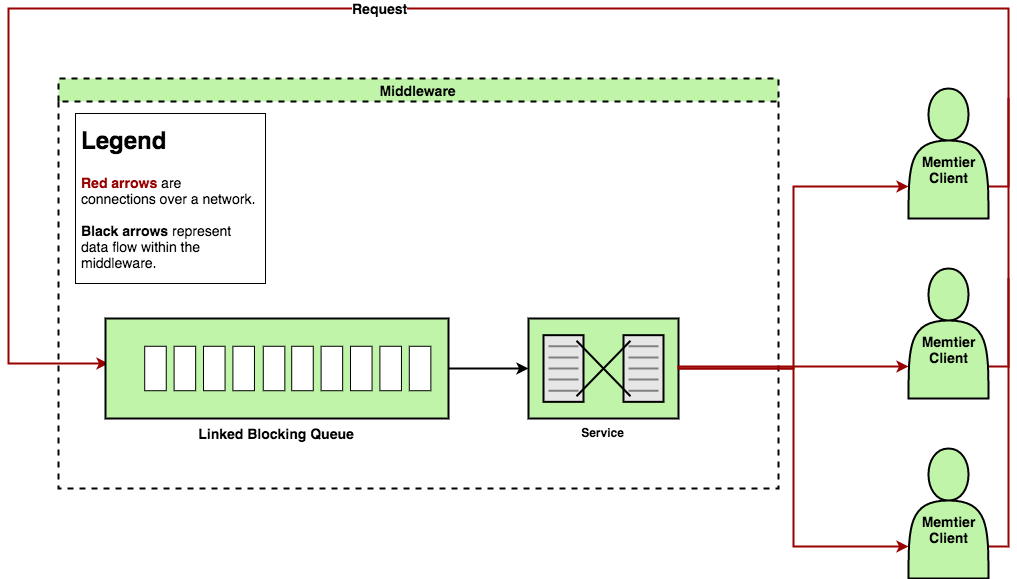
\includegraphics[width=\textwidth]{processing/graphics/mm1_queue.png}
    \caption{The middlewares modelled as an M/M/1 queue}
    \label{png::mm1_queue}
\end{figure}

The input to this model are the following:
\begin{enumerate}
    \item The \textit{service rate} will be computed from the mean service time at maximum throughput of the middlewares (shown in \ref{table::max_through_section_4}). The service time is computed from the difference between average response time measured on the middlewares and average queuing times (both taken at maximum throughput configurations). The inverse of this difference is then taken and multiplied by the total number of worker threads in the system. The result of this is used as the service rate.
    \item The throughput as measured by the middleware will be taken as the \textit{arrival rate}.
\end{enumerate}

The reasoning behind the choice of computation of these parameters is rather simple. For the service rate, due to the parallelism introduced by the workers, if a single worker thread were to perform the same work sequentially, it would require that thread to be exactly as many times faster than the average at there are workers in parallel. Hence the service time of this single worker can be computed by dividing the average service time of the parallel workers by the number of parallel workers. This is equivalent to multiplying the average service rate of the parallel workers by the total number of workers. Notice that this is the number of worker across the entire system, i.e. both middlewares. Therefore, in order to compute the service rate used in this subsection for the 8 worker configuration, the average service time measured during the experiment is multiplied by 16.

For the arrival rate, the reasoning is even more simplistic. As all virtual memtier clients will wait for a response from the middlewares before sending another request, it is trivial that the average throughput is equal to the average arrival rate.

Using these parameters, one obtains the data shown in tables \ref{table::mm1_data_8}, \ref{table::mm1_data_16}, \ref{table::mm1_data_32}, and \ref{table::mm1_data_64}. In these tables, \textbf{AR} denotes arrival rate, \textbf{SR} denotes service rate, \textbf{ST} denotes service time, \textbf{Util} denotes utilisation, \textbf{QL} denotes queue length, \textbf{QT} denotes queue time, and \textbf{RT} denotes response time.

\begin{table}
    \centering
    \resizebox{\textwidth}{!}{
        \begin{tabular}{|l|r|r|r|r|r|r|r|r|}
            \hline \multicolumn{8}{|c|}{\textbf{8 Workers (16 total)}} \\
            \hline \multicolumn{1}{|c|}{\textbf{Clients}} & \multicolumn{1}{|c|}{\textbf{AR}} & \multicolumn{1}{|c|}{\textbf{SR}} & \multicolumn{1}{|c|}{\textbf{ST (ms)}} & \multicolumn{1}{|c|}{\textbf{Util (\%)}} & \multicolumn{1}{|c|}{\textbf{QL}} & \multicolumn{1}{|c|}{\textbf{QT (ms)}} & \multicolumn{1}{|c|}{\textbf{RT (ms)}} \\
            \hline
            \hline 2 &   3714.358 &   6271.214 &    0.15946 &     59.229 &    0.86042 &    0.23165 &    0.39111 \\
            \hline 4 &   5998.812 &   6271.214 &    0.15946 &     95.656 &     21.065 &     3.5116 &     3.6711 \\
            \hline 8 &   6218.021 &   6271.214 &    0.15946 &     99.152 &      115.9 &      18.64 &       18.8 \\
            \hline 16 &   6207.667 &   6271.214 &    0.15946 &     98.987 &     96.696 &     15.577 &     15.736 \\
            \hline 24 &   6212.946 &   6271.214 &    0.15946 &     99.071 &     105.64 &     17.003 &     17.162 \\
            \hline 32 &   6198.538 &   6271.214 &    0.15946 &     98.841 &     84.301 &       13.6 &      13.76 \\
            \hline 40 &   6217.821 &   6271.214 &    0.15946 &     99.149 &     115.46 &      18.57 &     18.729 \\
            \hline 48 &   6202.592 &   6271.214 &    0.15946 &     98.906 &     89.399 &     14.413 &     14.573 \\
            \hline 56 &   6155.137 &   6271.214 &    0.15946 &     98.149 &     52.045 &     8.4556 &      8.615 \\
            \hline
        \end{tabular}
    }
    \caption{Data for M/M/1 queuing model for 8 worker configuration}
    \label{table::mm1_data_8}
\end{table}

In table \ref{table::mm1_data_8}, one can clearly see that the highest utilisation is reached with 8 clients per thread. This follows as it is the point of highest throughput found by the middleware. Moreover, nearly full utilisation is reached already at 4 clients per thread. This coincides with the point of saturation found during the analysis in section \ref{section::queue_model}. Queue lengths and therefore also queue time do not coincide at all with data measured by the middleware. This is due to the fact that the client count gives an upper bound to the number of requests in the system. Therefore, at say 8 clients per thread, there is not enough total clients (48) to even generate 115 requests simultaneously.

On the other hand, note that at higher client counts, the queue length is much lower than the ones given by the measurements. This is due the model design. A single worker has a different impact on a queue to 16 workers being 16 times slower.

As queue length impacts queue time, the queue times computed by the model do not match response times measured during the experiment. Similarly, as queue time impacts response time, the response times are very different to the measurements as well.

\begin{table}
    \centering
    \resizebox{\textwidth}{!}{
        \begin{tabular}{|l|r|r|r|r|r|r|r|r|}
            \hline \multicolumn{8}{|c|}{\textbf{16 Workers (32 total)}} \\
            \hline \multicolumn{1}{|c|}{\textbf{Clients}} & \multicolumn{1}{|c|}{\textbf{AR}} & \multicolumn{1}{|c|}{\textbf{SR}} & \multicolumn{1}{|c|}{\textbf{ST (ms)}} & \multicolumn{1}{|c|}{\textbf{Util (\%)}} & \multicolumn{1}{|c|}{\textbf{QL}} & \multicolumn{1}{|c|}{\textbf{QT (ms)}} & \multicolumn{1}{|c|}{\textbf{RT (ms)}} \\
            \hline
            \hline 2 &   3621.567 &   10692.54 &   0.093523 &      33.87 &    0.17347 &     0.0479 &    0.14142 \\
            \hline 4 &   6814.504 &   10692.54 &   0.093523 &     63.731 &     1.1199 &    0.16434 &    0.25786 \\
            \hline 8 &   9249.221 &   10692.54 &   0.093523 &     86.502 &     5.5433 &    0.59932 &    0.69285 \\
            \hline 16 &    10412.3 &   10692.54 &   0.093523 &     97.379 &     36.181 &     3.4749 &     3.5684 \\
            \hline 24 &    10259.3 &   10692.54 &   0.093523 &     95.948 &     22.721 &     2.2147 &     2.3082 \\
            \hline 32 &   10320.58 &   10692.54 &   0.093523 &     96.521 &     26.781 &     2.5949 &     2.6885 \\
            \hline 40 &    10164.5 &   10692.54 &   0.093523 &     95.062 &     18.299 &     1.8003 &     1.8938 \\
            \hline 48 &   10287.29 &   10692.54 &   0.093523 &      96.21 &     24.423 &     2.3741 &     2.4676 \\
            \hline 56 &   10623.76 &   10692.54 &   0.093523 &     99.357 &     153.46 &     14.445 &     14.538 \\
            \hline
        \end{tabular}
    }
    \caption{Data for M/M/1 queuing model for 16 worker configuration}
    \label{table::mm1_data_16}
\end{table}

Table \ref{table::mm1_data_16} illustrates the data obtained when applying the M/M/1 model to the system running two middlewares with 16 worker threads as a configuration. Once more, the system reaches near full utilisation at the same point saturation was observed during the experiment. Notice that this time queue lengths and queue times are reasonably accurate before the point of saturation. However, past that point they no longer match data gathered during the experiment.

Moreover, small changes in the utilisation result in very large changes in queue lengths when utilisation is close to 100\%. This is again due to the design of this model. As the model assumes only one very fast worker, reaching high utilisations has much more impact on the queue than when modelling with more workers.

\begin{table}
    \centering
    \resizebox{\textwidth}{!}{
        \begin{tabular}{|l|r|r|r|r|r|r|r|r|}
            \hline \multicolumn{8}{|c|}{\textbf{32 Workers (64 total)}} \\
            \hline \multicolumn{1}{|c|}{\textbf{Clients}} & \multicolumn{1}{|c|}{\textbf{AR}} & \multicolumn{1}{|c|}{\textbf{SR}} & \multicolumn{1}{|c|}{\textbf{ST (ms)}} & \multicolumn{1}{|c|}{\textbf{Util (\%)}} & \multicolumn{1}{|c|}{\textbf{QL}} & \multicolumn{1}{|c|}{\textbf{QT (ms)}} & \multicolumn{1}{|c|}{\textbf{RT (ms)}} \\
            \hline
            \hline 2 &   3725.717 &   13278.59 &   0.075309 &     28.058 &    0.10943 &   0.029371 &    0.10468 \\
            \hline 4 &   7082.292 &   13278.59 &   0.075309 &     53.336 &    0.60963 &   0.086078 &    0.16139 \\
            \hline 8 &   10030.78 &   13278.59 &   0.075309 &     75.541 &     2.3331 &    0.23259 &     0.3079 \\
            \hline 16 &   12332.62 &   13278.59 &   0.075309 &     92.876 &     12.108 &    0.98181 &     1.0571 \\
            \hline 24 &   12871.18 &   13278.59 &   0.075309 &     96.932 &     30.624 &     2.3792 &     2.4545 \\
            \hline 32 &   12993.27 &   13278.59 &   0.075309 &     97.851 &     44.561 &     3.4296 &     3.5049 \\
            \hline 40 &   13032.93 &   13278.59 &   0.075309 &      98.15 &     52.072 &     3.9954 &     4.0707 \\
            \hline 48 &    13175.4 &   13278.59 &   0.075309 &     99.223 &     126.69 &     9.6159 &     9.6912 \\
            \hline 56 &   12834.42 &   13278.59 &   0.075309 &     96.655 &     27.929 &     2.1761 &     2.2514 \\
            \hline
        \end{tabular}
    }
    \caption{Data for M/M/1 queuing model for 32 worker configuration}
    \label{table::mm1_data_32}
\end{table}

Table \ref{table::mm1_data_32} shows utilisation levels above 90\% for 16 clients per thread and above. This is also the point of saturation observed during experiments. For the rest of the data, the same analysis as given for 16 workers can be applied here.


\begin{table}
    \centering
    \resizebox{\textwidth}{!}{
        \begin{tabular}{|l|r|r|r|r|r|r|r|r|}
            \hline \multicolumn{8}{|c|}{\textbf{64 Workers (128 total)}} \\
            \hline \multicolumn{1}{|c|}{\textbf{Clients}} & \multicolumn{1}{|c|}{\textbf{AR}} & \multicolumn{1}{|c|}{\textbf{SR}} & \multicolumn{1}{|c|}{\textbf{ST (ms)}} & \multicolumn{1}{|c|}{\textbf{Util (\%)}} & \multicolumn{1}{|c|}{\textbf{QL}} & \multicolumn{1}{|c|}{\textbf{QT (ms)}} & \multicolumn{1}{|c|}{\textbf{RT (ms)}} \\
            \hline
            \hline 2 &   3712.546 &    15590.7 &   0.064141 &     23.813 &   0.074427 &   0.020047 &   0.084188 \\
            \hline 4 &   7000.029 &    15590.7 &   0.064141 &     44.899 &    0.36585 &   0.052265 &    0.11641 \\
            \hline 8 &     9851.5 &    15590.7 &   0.064141 &     63.188 &     1.0846 &     0.1101 &    0.17424 \\
            \hline 16 &   12849.02 &    15590.7 &   0.064141 &     82.415 &     3.8624 &     0.3006 &    0.36474 \\
            \hline 24 &   13445.12 &    15590.7 &   0.064141 &     86.238 &     5.4041 &    0.40194 &    0.46608 \\
            \hline 32 &   13990.43 &    15590.7 &   0.064141 &     89.736 &     7.8452 &    0.56076 &     0.6249 \\
            \hline 40 &   14844.52 &    15590.7 &   0.064141 &     95.214 &     18.942 &      1.276 &     1.3402 \\
            \hline 48 &   15243.51 &    15590.7 &   0.064141 &     97.773 &     42.929 &     2.8162 &     2.8803 \\
            \hline 56 &   15421.14 &    15590.7 &   0.064141 &     98.912 &      89.96 &     5.8335 &     5.8977 \\
            \hline
        \end{tabular}
    }
    \caption{Data for M/M/1 queuing model for 64 worker configuration}
    \label{table::mm1_data_64}
\end{table}

The data illustrated in table \ref{table::mm1_data_64} shows the M/M/1 model applied to the system with a configuration of 64 workers per middleware. As close to full utilisation is reached much later, queue lengths computed here are much more accurate. However, response times are not accurate at all. This is caused by the fact that service times are much higher than used in the model. In fact, the real average service rate is nearly three milliseconds longer than the response time given in the last row of table \ref{table::mm1_data_64}.

\subsection{M/M/m}

\begin{figure}[!h]
    \centering
    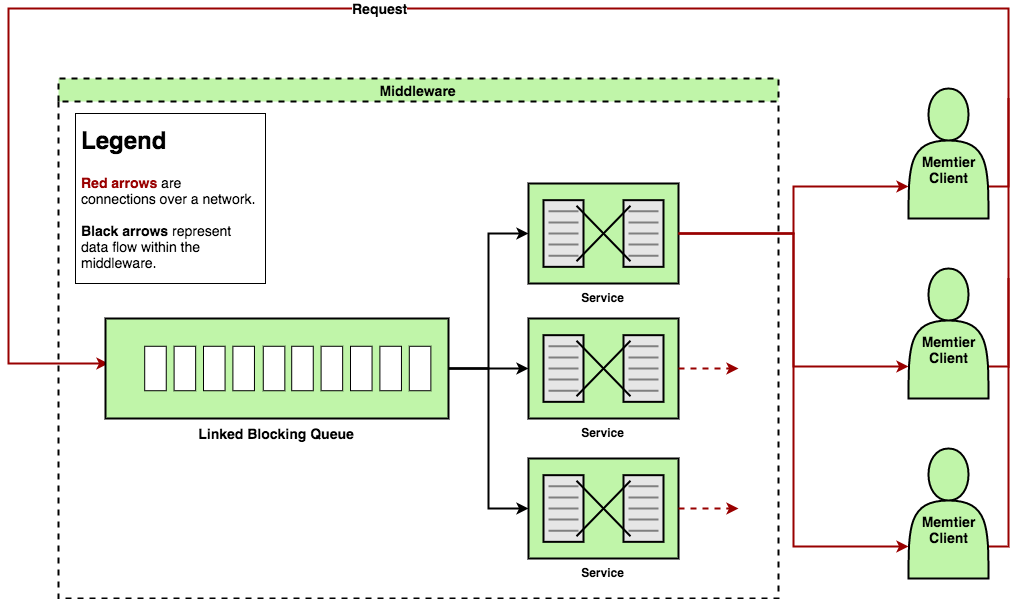
\includegraphics[width=\textwidth]{processing/graphics/mmn_queue.png}
    \caption{The middlewares modelled as an M/M/m queue}
    \label{png::mmn_queue}
\end{figure}

Figure \ref{png::mmn_queue} illustrates the model used in this subsection. A variable amount of services are run in parallel. These services are worker threads and their number varies from one configuration to another. Note that a single queue is still used instead of two distinct ones as in the real system (one for each middleware). The input to this model are the following:

\begin{enumerate}
    \item The \textit{service rate} is computed from the mean service time at maximum throughput of the middlewares. The average service time is computed as for the M/M/1 model. Then it's inverse is taken as the service rate.
    \item The arrival rate is computed as for the M/M/1 model.
\end{enumerate}

The server count ($m$) used for the model is equal to twice the number of worker threads used in the configurations. This follows from the way the service rate was computed. As the service rate taken from the average service times of a worker, the total number of workers in the system (twice the number given in the configuration as two middlewares are used) serves as the count of service providing entities for the model.

\begin{table}
    \centering
    \resizebox{\textwidth}{!}{
        \begin{tabular}{|l|r|r|r|r|r|r|r|r|}
            \hline \multicolumn{8}{|c|}{\textbf{8 Workers (16 total)}} \\
            \hline \multicolumn{1}{|c|}{\textbf{Clients}} & \multicolumn{1}{|c|}{\textbf{AR}} & \multicolumn{1}{|c|}{\textbf{SR}} & \multicolumn{1}{|c|}{\textbf{ST (ms)}} & \multicolumn{1}{|c|}{\textbf{Util (\%)}} & \multicolumn{1}{|c|}{\textbf{QL}} & \multicolumn{1}{|c|}{\textbf{QT (ms)}} & \multicolumn{1}{|c|}{\textbf{RT (ms)}} \\
            \hline
            \hline 2 &   3714.358 &   391.9509 &     2.5513 &     59.229 &   0.054926 &   0.014787 &     2.5661 \\
            \hline 4 &   5998.812 &   391.9509 &     2.5513 &     95.656 &     17.778 &     2.9636 &     5.5149 \\
            \hline 8 &   6218.021 &   391.9509 &     2.5513 &     99.152 &     112.28 &     18.058 &     20.609 \\
            \hline 16 &   6207.667 &   391.9509 &     2.5513 &     98.987 &     93.091 &     14.996 &     17.548 \\
            \hline 24 &   6212.946 &   391.9509 &     2.5513 &     99.071 &     102.02 &     16.421 &     18.972 \\
            \hline 32 &   6198.538 &   391.9509 &     2.5513 &     98.841 &      80.71 &     13.021 &     15.572 \\
            \hline 40 &   6217.821 &   391.9509 &     2.5513 &     99.149 &     111.84 &     17.987 &     20.539 \\
            \hline 48 &   6202.592 &   391.9509 &     2.5513 &     98.906 &     85.802 &     13.833 &     16.385 \\
            \hline 56 &   6155.137 &   391.9509 &     2.5513 &     98.149 &     48.521 &      7.883 &     10.434 \\
            \hline
        \end{tabular}
    }
    \caption{Data for M/M/16 queuing model for 8 worker configuration}
    \label{table::mmn_data_8}
\end{table}

Table \ref{table::mmn_data_8} shows the data for a M/M/16 model based on arrival rates and service rates computed from the data measured at maximum throughput for this configuration. Notice that utilisation computed using this model is exactly equal to utilisations computed by the M/M/1 models (see figure \ref{table::mm1_data_8}). This immediately follows from the way service rates were computed.

Moreover, notice that response times no longer approach zero as clients decrease. This is caused as the service time provides a lower bound and M/M/m models provide more realistic approximations of service times. However, generally speaking, this does not results in accurate response times, queue length, or queue times. The actual service time increases as more load is put onto the system. Therefore, the constant service time cannot provide a realistic enough model to accurately approximate response times and queue lengths. On the other hand, as the service time for 8 workers is the most stable one, response times for low load configurations given by the model are actually relatively close to the real values. This is no longer observable for configurations with more workers as service rates vary greatly as more load is added.

\begin{table}
    \centering
    \resizebox{\textwidth}{!}{
        \begin{tabular}{|l|r|r|r|r|r|r|r|r|}
            \hline \multicolumn{8}{|c|}{\textbf{16 Workers (32 total)}} \\
            \hline \multicolumn{1}{|c|}{\textbf{Clients}} & \multicolumn{1}{|c|}{\textbf{AR}} & \multicolumn{1}{|c|}{\textbf{SR}} & \multicolumn{1}{|c|}{\textbf{ST (ms)}} & \multicolumn{1}{|c|}{\textbf{Util (\%)}} & \multicolumn{1}{|c|}{\textbf{QL}} & \multicolumn{1}{|c|}{\textbf{QT (ms)}} & \multicolumn{1}{|c|}{\textbf{RT (ms)}} \\
            \hline
            \hline 2 &   3621.567 &   334.1419 &     2.9927 &      33.87 & 7.5977e-08 & 2.0979e-08 &     2.9927 \\
            \hline 4 &   6814.504 &   334.1419 &     2.9927 &     63.731 &   0.020496 &  0.0030077 &     2.9957 \\
            \hline 8 &   9249.221 &   334.1419 &     2.9927 &     86.502 &     2.1091 &    0.22803 &     3.2208 \\
            \hline 16 &    10412.3 &   334.1419 &     2.9927 &     97.379 &     30.912 &     2.9688 &     5.9615 \\
            \hline 24 &    10259.3 &   334.1419 &     2.9927 &     95.948 &     17.717 &     1.7269 &     4.7197 \\
            \hline 32 &   10320.58 &   334.1419 &     2.9927 &     96.521 &     21.672 &     2.0999 &     5.0926 \\
            \hline 40 &    10164.5 &   334.1419 &     2.9927 &     95.062 &     13.456 &     1.3238 &     4.3166 \\
            \hline 48 &   10287.29 &   334.1419 &     2.9927 &      96.21 &     19.371 &      1.883 &     4.8757 \\
            \hline 56 &   10623.76 &   334.1419 &     2.9927 &     99.357 &     147.81 &     13.913 &     16.906 \\
            \hline
        \end{tabular}
    }
    \caption{Data for M/M/32 queuing model for 16 worker configuration}
    \label{table::mmn_data_16}
\end{table}

The data displayed in table \ref{table::mmn_data_16} can be analysed in a very similar fashion to the M/M/16 model above. As previously said, response times for low loads are no longer accurate. The instability in service rates is nearly exclusively due to increases in server times for more load. As more load is available due to higher client counts and more worker threads running in parallel, requests stagnate in the memcached servers, making server times longer for the middleware. As these server times are included in the service time, the latter also increase. Therefore, response times for low loads can actually much shorter than the service times given at highest throughput setups.

\begin{table}
    \centering
    \resizebox{\textwidth}{!}{
        \begin{tabular}{|l|r|r|r|r|r|r|r|r|}
            \hline \multicolumn{8}{|c|}{\textbf{32 Workers (64 total)}} \\
            \hline \multicolumn{1}{|c|}{\textbf{Clients}} & \multicolumn{1}{|c|}{\textbf{AR}} & \multicolumn{1}{|c|}{\textbf{SR}} & \multicolumn{1}{|c|}{\textbf{ST (ms)}} & \multicolumn{1}{|c|}{\textbf{Util (\%)}} & \multicolumn{1}{|c|}{\textbf{QL}} & \multicolumn{1}{|c|}{\textbf{QT (ms)}} & \multicolumn{1}{|c|}{\textbf{RT (ms)}} \\
            \hline
            \hline 2 &   3725.717 &   207.4779 &     4.8198 &     28.058 & 1.2683e-17 &  3.404e-18 &     4.8198 \\
            \hline 4 &   7082.292 &   207.4779 &     4.8198 &     53.336 & 3.8535e-06 & 5.4411e-07 &     4.8198 \\
            \hline 8 &   10030.78 &   207.4779 &     4.8198 &     75.541 &   0.063017 &  0.0062823 &     4.8261 \\
            \hline 16 &   12332.62 &   207.4779 &     4.8198 &     92.876 &     5.9315 &    0.48096 &     5.3008 \\
            \hline 24 &   12871.18 &   207.4779 &     4.8198 &     96.932 &     23.068 &     1.7922 &      6.612 \\
            \hline 32 &   12993.27 &   207.4779 &     4.8198 &     97.851 &     36.671 &     2.8223 &     7.6421 \\
            \hline 40 &   13032.93 &   207.4779 &     4.8198 &      98.15 &      44.07 &     3.3814 &     8.2012 \\
            \hline 48 &    13175.4 &   207.4779 &     4.8198 &     99.223 &     118.29 &     8.9779 &     13.798 \\
            \hline 56 &   12834.42 &   207.4779 &     4.8198 &     96.655 &     20.473 &     1.5951 &     6.4149 \\
            \hline
        \end{tabular}
    }
    \caption{Data for M/M/64 queuing model for 32 worker configuration}
    \label{table::mmn_data_32}
\end{table}

Table \ref{table::mmn_data_32} shows the same issues as the two before. The response time computed by the model is too low until 16 clients per thread and then it does not increase enough compared to the real values.

\begin{table}
    \centering
    \resizebox{\textwidth}{!}{
        \begin{tabular}{|l|r|r|r|r|r|r|r|r|}
            \hline \multicolumn{8}{|c|}{\textbf{64 Workers (128 total)}} \\
            \hline \multicolumn{1}{|c|}{\textbf{Clients}} & \multicolumn{1}{|c|}{\textbf{AR}} & \multicolumn{1}{|c|}{\textbf{SR}} & \multicolumn{1}{|c|}{\textbf{ST (ms)}} & \multicolumn{1}{|c|}{\textbf{Util (\%)}} & \multicolumn{1}{|c|}{\textbf{QL}} & \multicolumn{1}{|c|}{\textbf{QT (ms)}} & \multicolumn{1}{|c|}{\textbf{RT (ms)}} \\
            \hline
            \hline 2 &   3712.546 &   121.8023 &       8.21 &     23.813 & 5.5415e-40 & 1.4926e-40 &       8.21 \\
            \hline 4 &   7000.029 &   121.8023 &       8.21 &     44.899 & 6.8162e-16 & 9.7374e-17 &       8.21 \\
            \hline 8 &     9851.5 &   121.8023 &       8.21 &     63.188 & 1.4478e-06 & 1.4696e-07 &       8.21 \\
            \hline 16 &   12849.02 &   121.8023 &       8.21 &     82.415 &   0.099012 &  0.0077058 &     8.2177 \\
            \hline 24 &   13445.12 &   121.8023 &       8.21 &     86.238 &    0.41633 &   0.030965 &      8.241 \\
            \hline 32 &   13990.43 &   121.8023 &       8.21 &     89.736 &     1.3906 &   0.099393 &     8.3094 \\
            \hline 40 &   14844.52 &   121.8023 &       8.21 &     95.214 &     9.4545 &     0.6369 &     8.8469 \\
            \hline 48 &   15243.51 &   121.8023 &       8.21 &     97.773 &     31.719 &     2.0808 &     10.291 \\
            \hline 56 &   15421.14 &   121.8023 &       8.21 &     98.912 &     77.925 &     5.0531 &     13.263 \\
            \hline
        \end{tabular}
    }
    \caption{Data for M/M/128 queuing model for 64 worker configuration}
    \label{table::mmn_data_64}
\end{table}

The queue lengths in table \ref{table::mmn_data_64} are the correct order of magnitude. However, with the exception of the last row of the table, queue length still have a significant error (easily reaching over 100\% deviations to the real values).


\subsection{Network of Queues}
Figure \ref{png::network_queues_1mw} shows the system from section \ref{section::net_queues} with a single middleware. The queue considered in the middleware is the same as for the M/M/m models. However, note that each client instance and instance of memcached also has a queue. The queue for memecached models the internal queue used by memcached. In the specifications of memcached, one can read that when launching with a single thread (as performed during the experiments), memcached uses a listener thread to listen to requests and stores to a queue. The single worker thread then processes requests on the queue.

The motivation behind the queue used for the memtier instances is very similar. As numerous worker threads are used in the middleware, memtier can receive more than two responses simultaneously. However, because at most two threads are used in memtier, not all responses can be handled immediately. Hence creating a queueing situation.

Figure \ref{png::network_queues_2mw} shows the same model but with two separate middlewares.

\begin{SidewaysFigure}
    \centering
    \begin{minipage}[b]{0.9\paperheight}
        \centering
        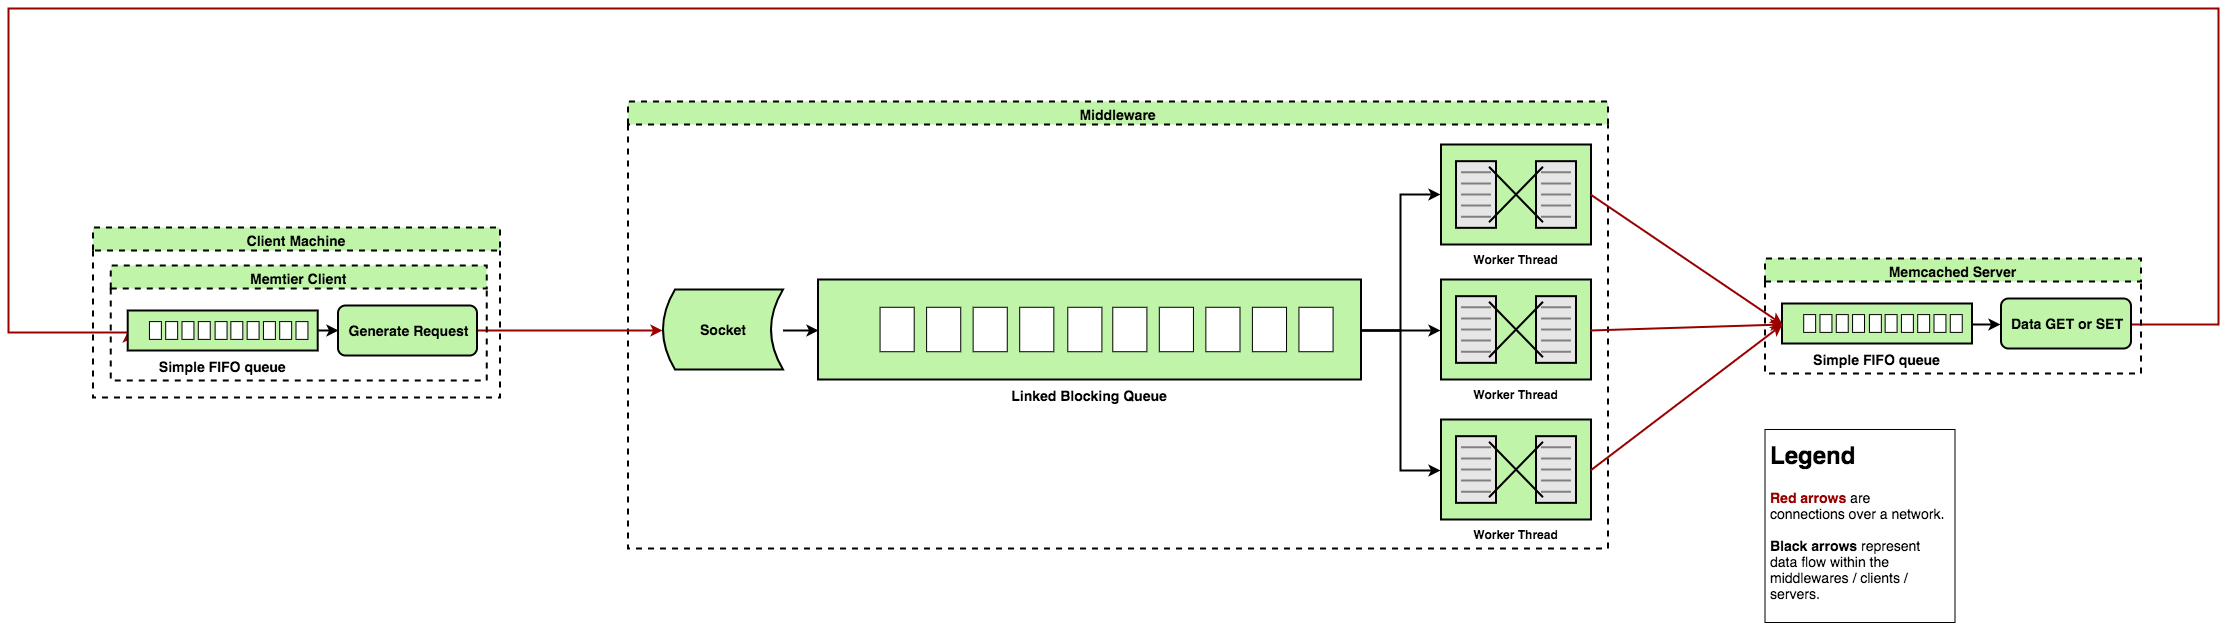
\includegraphics[width=0.65\paperheight]{processing/graphics/network_queues_1mw.png}
        \caption{System modelled as a network of queues for a single middleware}
        \label{png::network_queues_1mw}
    \end{minipage}

    \hfill
    \vspace*{1cm}

    \begin{minipage}[b]{0.9\paperheight}
        \centering
        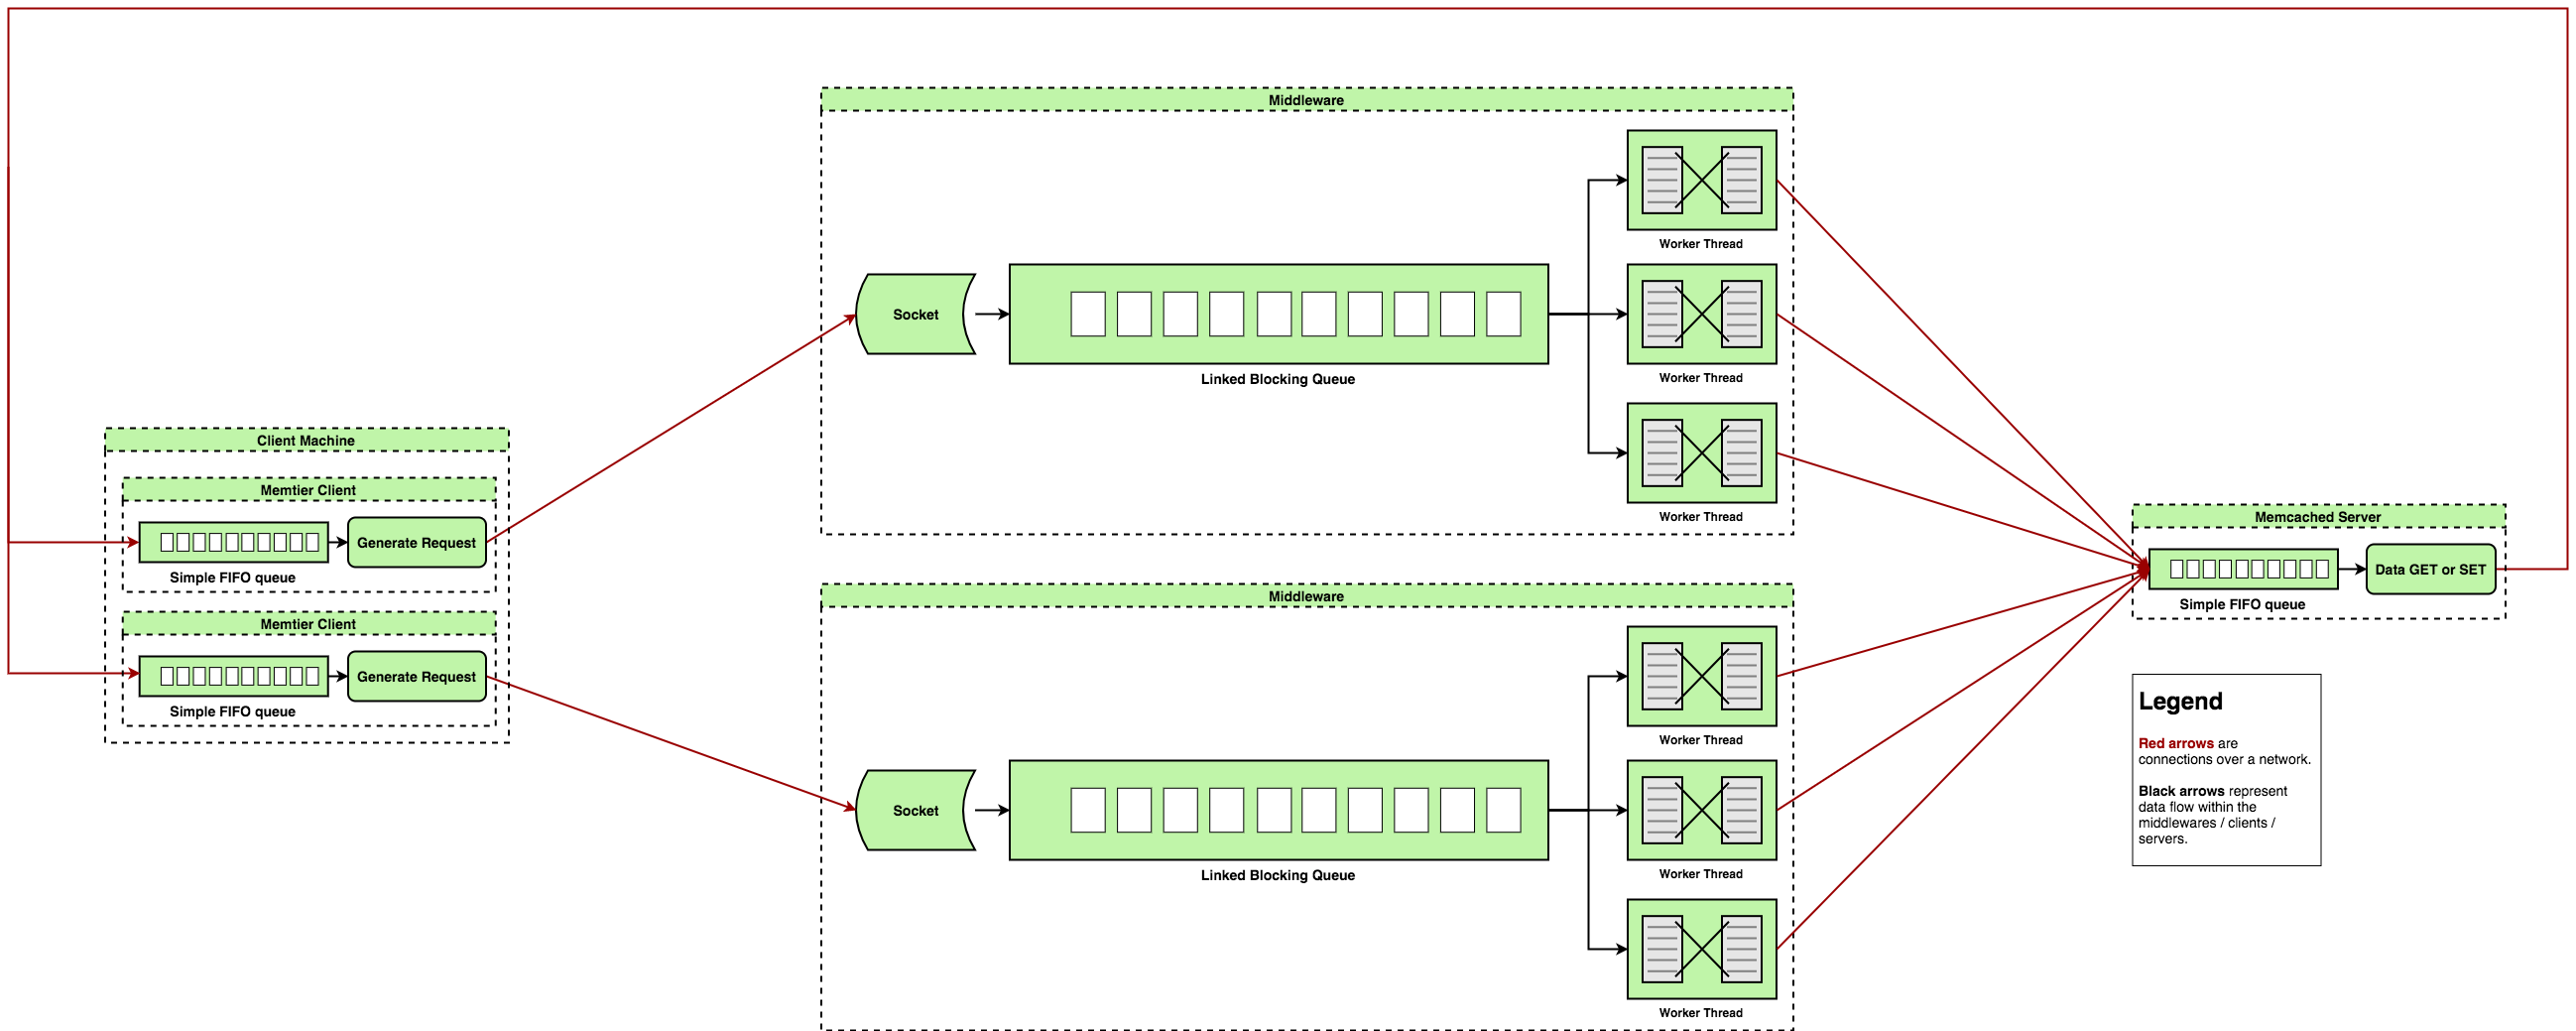
\includegraphics[width=0.65\paperheight]{processing/graphics/network_queues_2mw.png}
        \caption{System modelled as a network of queues for two middlewares}
        \label{png::network_queues_2mw}
    \end{minipage}
\end{SidewaysFigure}



The data flow represented in these schemas is not accurate as no flow leads back from the servers to the middleware. As the model does not consider any queue when data is passed back from the servers to the middleware, the flow is represented as going directly from the server to the clients.

\subsubsection{Single middleware}
First, note that the system is closed. No data is passed out of the system, and no data arrives from the outside.

Second, the number of requests per job is exactly one in each device. This would be different for sets and sharded multigets when using several backend servers. However, as only a single memcached server is used, each job spawns only a single request across all devices in the entire system.

Third, as all but the middleware use a M/M/1 model and the data flow as no fork between individual queuing models, the visit count for each device is exactly one. Moreover, the visit count for each service in each device is one, with the exception of the workers in the middleware, where the average visit count is one over the number of workers used in the middleware device.

Fourth, the total number of jobs in the system is taken as the average throughput as measured by the client. As no jobs are lost, no jobs are received from outside the system, and no jobs are sent outside the system, the average throughput as measured by the client can also be used as the average arrival rate for each device.

Finally, in order to compute properties of individual devices in the system, their respective response time will be used. As memtier does not involve any think time, one can assume that the cycle time across the system is the response time as measured by the clients. Then, by the forced flow law, the sum of individual response times from each device is equal to the response time measured by the client. Furthermore, the response time for the backend server is known as it is measured as the server time by the middleware. Moreover, the time a requests spends in the middleware is known as it can be computed by the time between reception of a request from a client and the time the request is completed. As the server is considered a separate device in this model, the server time can be deducted from this time interval to compute the time spend either in queue or processing in a worker within the middleware. The resulting time give the response time of the middleware. Thus, by the forced flow law, the response time of the client machine can be computed by subtracting the middleware's and the server's response times from the system response time.

The service time of the middleware can be observed from the measured timestamps. This usually varies between 0.032 and 0.047 milliseconds\footnote{\label{source::q_network}\mintinline{shell}{processing/final/queuing_model/network.xlsx}}, depending on load. In the case of the server and the client, service times can be computed the following way:
\begin{align}
    E[r] &= \frac{1/\mu}{1 - \rho}\\
    E[r] \cdot\mu &= \frac{1}{1 - \rho}\\
    \frac{1}{E[r]\cdot\mu} &= 1 - \rho\\
    \frac{1}{E[r]\cdot\mu} &= 1 - \frac{\lambda}{\mu}\\
    \frac{\lambda}{\mu} &= 1 - \frac{1}{E[r]\cdot\mu}\\
    \lambda &= \mu - \frac{1}{E[r]}\\
    \mu &= \lambda + \frac{1}{E[r]}\\
    \frac{1}{S} &= \lambda + \frac{1}{E[r]}\\
    S &= \frac{1}{\lambda + \frac{1}{E[r]}} \label{eq::service_time}
\end{align}
where $S$ is the service time, $E[r]$ the expected response time, $\lambda$ the arrival rate, and $\mu$ the service rate.

Obviously, this does not account for any network latencies between passing from one device to another. However, as the baselines for the performance of both clients and servers have been measured in a previous section, one can tell whether the performance is bound by the network or a client/server device.

Using the service time as explained above, the utilisation law can be used in order to compute utilisation of devices. Moreover, Little's law allows to compute the mean number of jobs in each device. This permits to model the middleware's queuing lengths.

\paragraph{Queue lengths}
Using Little's law, the queue times in the middleware can be computed. This is achieved by taking the average time spent in the middleware (without server time) and multiplying it by the system throughput. The reason the system throughput can be used is because the average visit count of a job in the middleware is exactly one. This gives very good approximations of the middleware's queue lengths\footref{source::q_network}. Note this computation does not take into account that workers may be processing requests, hence removing them from the queue. The reason this is not considered is due to the fact that close to the entirety of a workers processing time is taken up by server times, during which, according to the model, the request is not in the middleware anymore.

\paragraph{Worker utilisation}
The average visit count for a single worker is one over the total number of workers used in the middleware. Hence, using the forced flow law, one can compute the service demand and utilisation of the workers. This reaches a maximum at 8 workers, eighty total clients, and get operations with only 3.07 percent utilisation\footref{source::q_network}. Therefore the workers clearly do not represent a bottleneck.

\paragraph{Memcached server}
Using equation \ref{eq::service_time}, the service time of the server can be computed, hence allowing to also compute its utilisation. Figures \ref{png::q_network_svr_util_1mw_reads} and \ref{png::q_network_svr_util_1mw_writes} show the computed utilisation based on total client count for all worker configurations. One can clearly observe that utilisation reaches very high levels as the system saturates. However, the baselines without the middleware showed that higher levels of throughput were possible for a single memcached server. Therefore, the high utilisation shown on the graphs is a result of network latencies. These latencies are not considered in the model design but are included in the server's response time.
\begin{figure}[!h]
    \centering
    \begin{minipage}[b]{.45\textwidth}
        \centering
        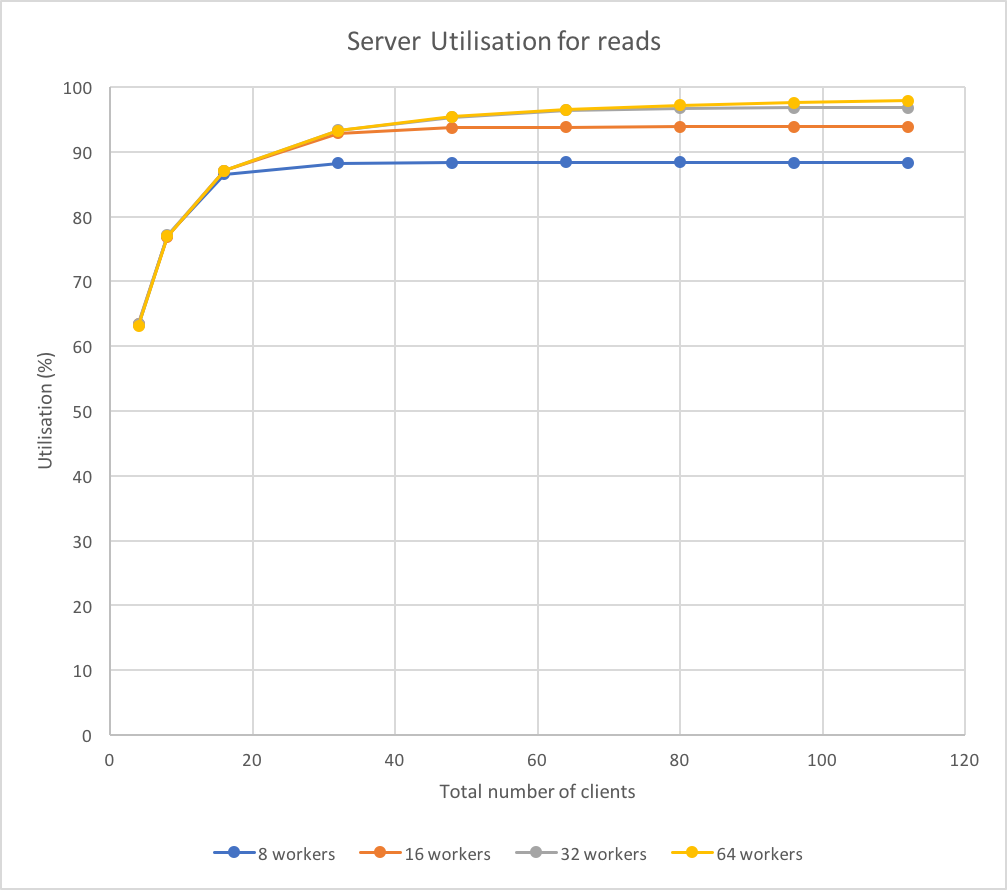
\includegraphics[width=\textwidth]{processing/graphics/q_network_svr_util_1mw_reads.png}
        \caption{Memcached server utilisation for reads}
        \label{png::q_network_svr_util_1mw_reads}
    \end{minipage}
    \qquad
    \begin{minipage}[b]{.45\textwidth}
        \centering
        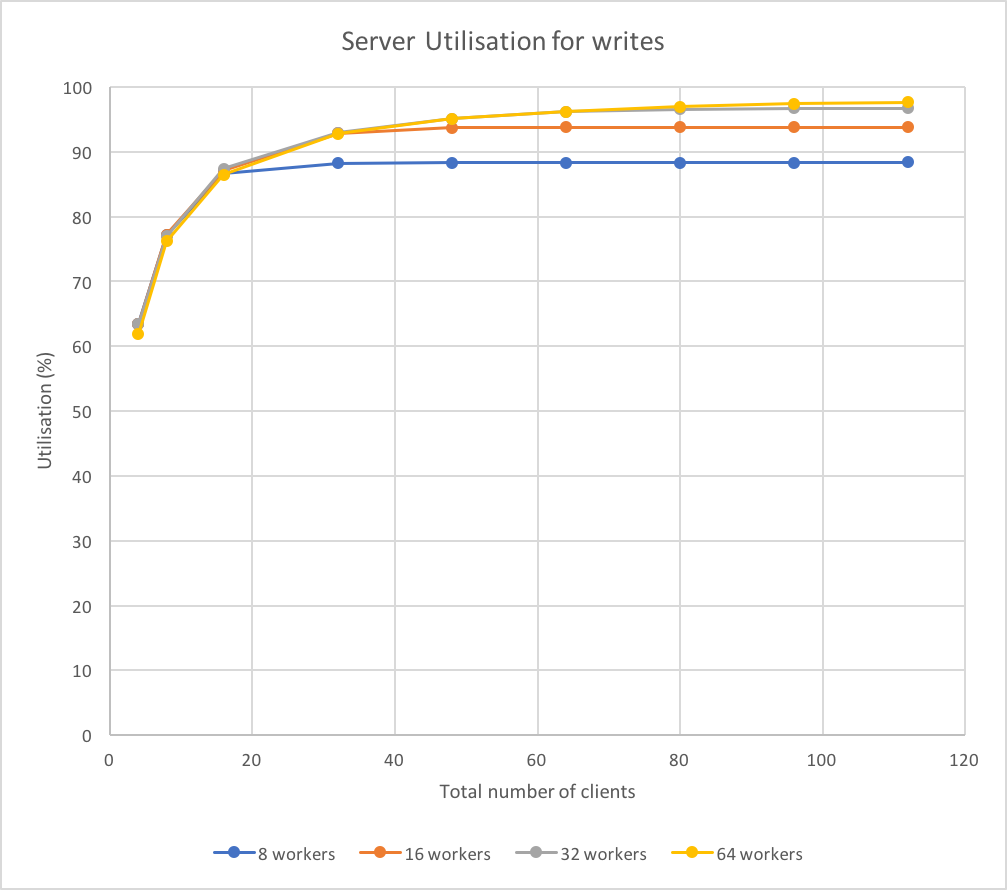
\includegraphics[width=\textwidth]{processing/graphics/q_network_svr_util_1mw_writes.png}
        \caption{Memcached server utilisation for writes}
        \label{png::q_network_svr_util_1mw_writes}
    \end{minipage}
\end{figure}


\paragraph{Memtier client}
Using the same equation as for the server, one can compute the utilisation of clients. Figures \ref{png::q_network_clt_util_1mw_reads} and \ref{png::q_network_clt_util_1mw_writes} show the utilisation of clients. Clients also reach very high utilisation levels. However, similarly to memcached, the baselines at the beginning of this report clearly show that clients can handle much more requests per seconds than the number of jobs in the system during these experiments. Again, network latencies are included in the utilisation computation as they are included in the response time computed for clients. Therefore, the actual bottleneck here is the network.
\begin{figure}[!h]
    \centering
    \begin{minipage}[b]{.45\textwidth}
        \centering
        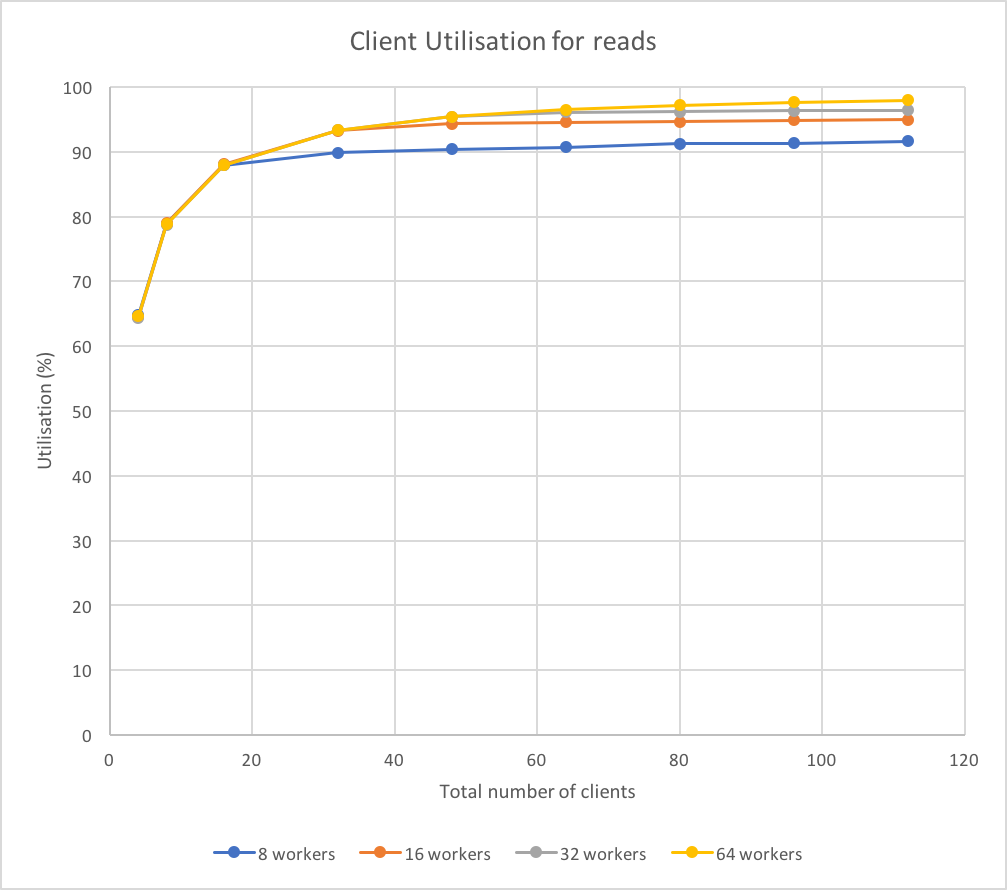
\includegraphics[width=\textwidth]{processing/graphics/q_network_clt_util_1mw_reads.png}
        \caption{Memtier client utilisation for reads}
        \label{png::q_network_clt_util_1mw_reads}
    \end{minipage}
    \qquad
    \begin{minipage}[b]{.45\textwidth}
        \centering
        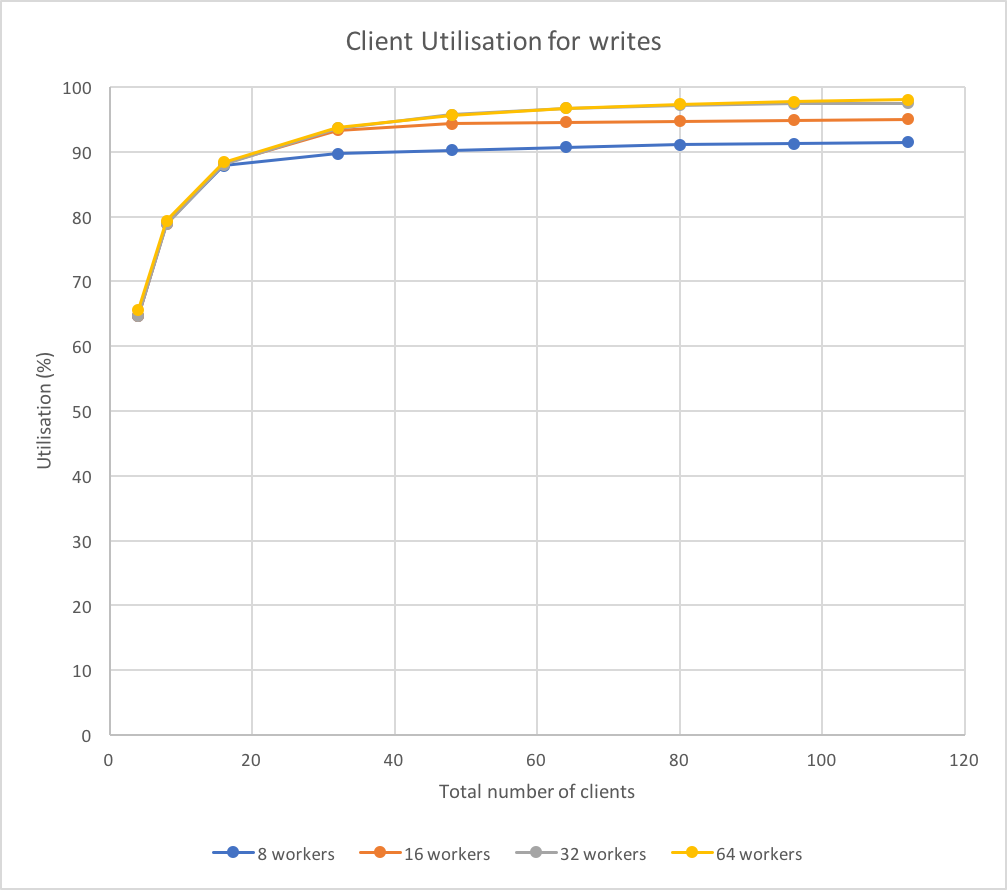
\includegraphics[width=\textwidth]{processing/graphics/q_network_clt_util_1mw_writes.png}
        \caption{Memtier client utilisation for writes}
        \label{png::q_network_clt_util_1mw_writes}
    \end{minipage}
\end{figure}

\paragraph{Summary}
There is no significant difference in utilisation between the client and the server. The service times computed using equation \ref{eq::service_time} are nearly equal for the client and the server. Moreover, their visit count is exactly one hence resulting in very similar service demand. This indicates that they present a comparable bottleneck (using bottleneck analysis as service demand is proportional to utilisation). This implies that the overall bottleneck in this system is the network.


\subsubsection{Two middlewares}
Just as for the single middleware model, the system under consideration is closed. However, in contrast to the model above, the visit count in each device is no longer one. In the case of the clients and the middlewares, the client count is one half. Therefore, even though the computations for measurements are performed very similarly for this model compared to the one presented above, they are not the same. For example, the average throughput of a single middleware is only half the measured throughput from the clients. This follows as throughputs from individual clients were added in post-processing to get the overall throughput of the system.

Server service times and client service times computations can remain unchanged. In the server case this is obvious as the queuing model does not change between single and two middleware models. In the case of clients, half the system's throughput must be taken as the arrival rate as the job visit count for each client instance is only one half.

\paragraph{Queue lengths}
Using Little's law the average queue length between the two middlewares can be computed. These estimates are very accurate\footnote{\label{source::q_network}\mintinline{shell}{processing/final/queuing_model/network.xlsx}}. Table \ref{talbe::ql_comparison} shows the values for the model compared to the measured values for eight worker read configurations.
\begin{table}
    \centering
    \begin{tabular}{|l|r|r|}
        \hline\multicolumn{1}{|c|}{\textbf{Clients}} & \multicolumn{1}{|c|}{\textbf{Queue Length Measured}} & \multicolumn{1}{|c|}{\textbf{Queue Length computed}} \\
        \hline\hline 4 & 0.083333333 & 0.124644061 \\
        \hline 8 & 0.214583333 & 0.313031324 \\
        \hline 16 & 0.514583333 & 0.683040185 \\
        \hline 32 & 2.9875 & 2.984606201 \\
        \hline 48 & 9.329166667 & 9.740633864 \\
        \hline 64 & 17.5375 & 17.49674752 \\
        \hline 80 & 24.92291667 & 25.46997539 \\
        \hline 96 & 33.11666667 & 33.39988338 \\
        \hline 112 & 40.24583333 & 41.34618177 \\
        \hline
    \end{tabular}
    \caption{Queue length model comparison}
    \source{processing/final/queuing\_model/network.xlsx}
    \label{talbe::ql_comparison}
\end{table}

\paragraph{Worker utilisation}
Worker utilisation is even lower than in the single middleware model. This was to be expected, as throughput does not double but the number of total workers (across both middleware) doubles. This once again shows that workers do not present a bottleneck.

\paragraph{Memcached server}
Figures \ref{png::q_network_svr_util_2mw_reads} and \ref{png::q_network_svr_util_2mw_writes} show server utilisations for reads and writes respectively. Notice that server utilisations reach higher levels than for the single middleware model. This is caused by an increased load on the server. However, note that, still, lower worker configurations result in lower utilisation, indicating the network is still the bottleneck.
\begin{figure}[!h]
    \centering
    \begin{minipage}[b]{.45\textwidth}
        \centering
        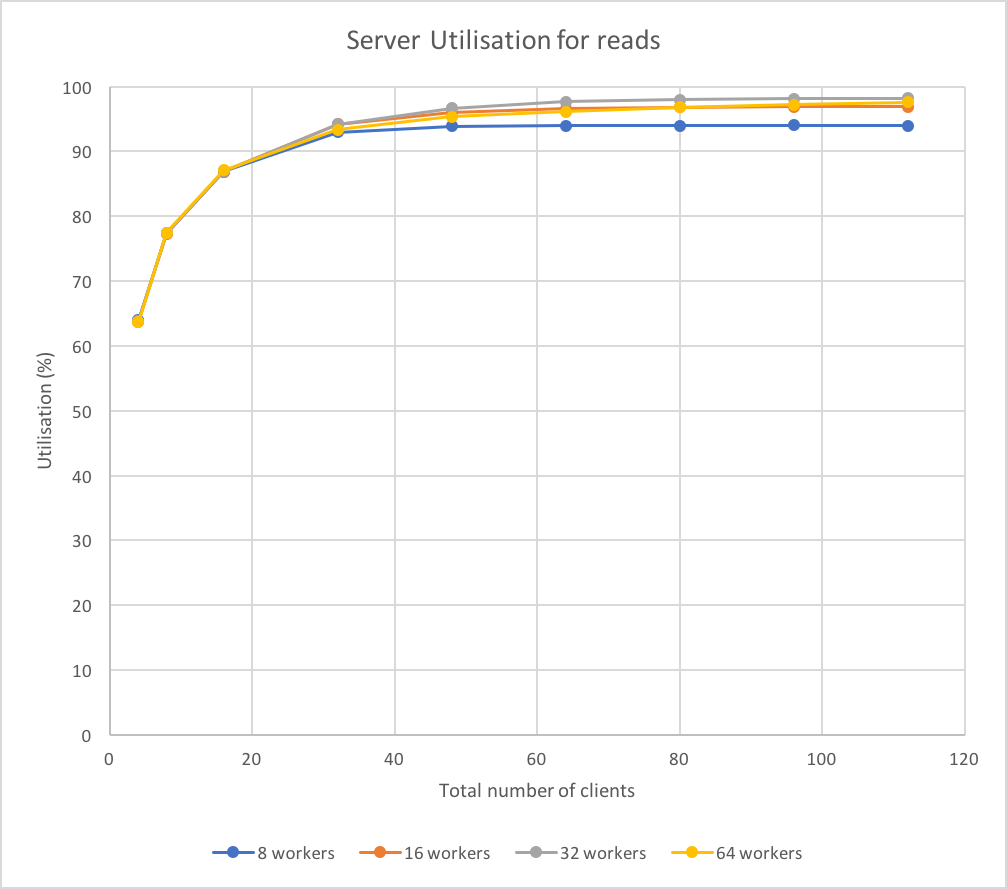
\includegraphics[width=\textwidth]{processing/graphics/q_network_svr_util_2mw_reads.png}
        \caption{Memcached server utilisation for reads}
        \label{png::q_network_svr_util_2mw_reads}
    \end{minipage}
    \qquad
    \begin{minipage}[b]{.45\textwidth}
        \centering
        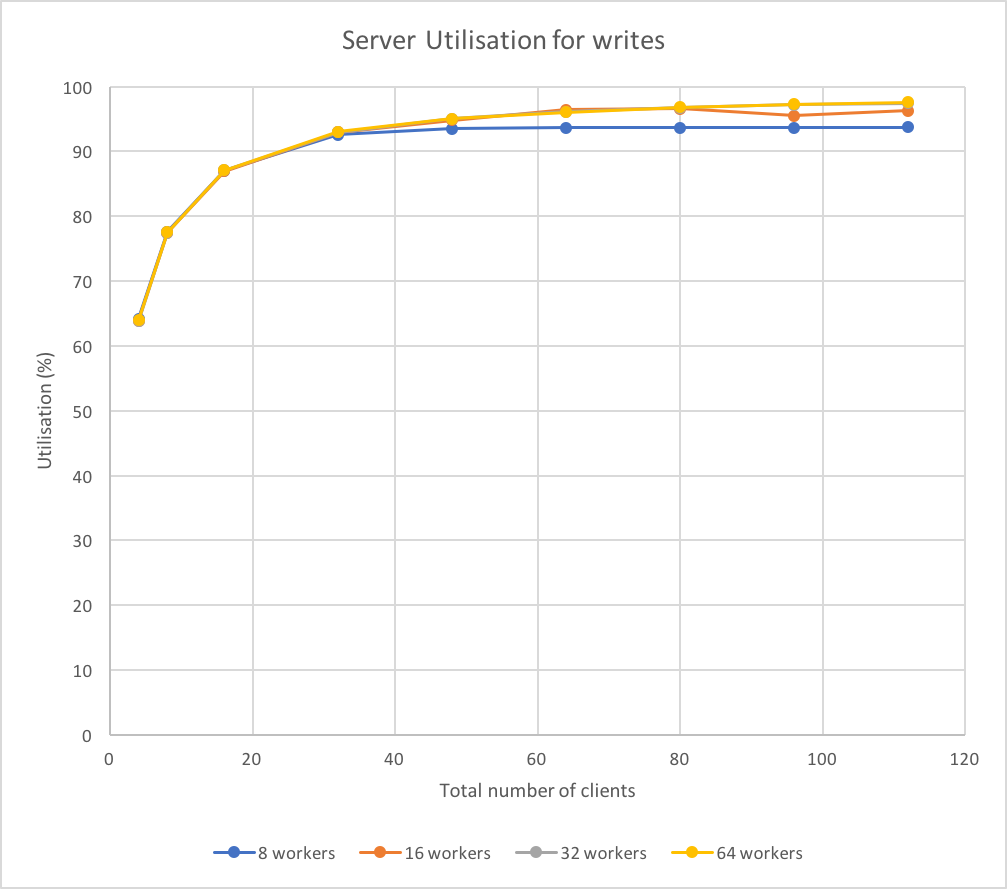
\includegraphics[width=\textwidth]{processing/graphics/q_network_svr_util_2mw_writes.png}
        \caption{Memcached server utilisation for writes}
        \label{png::q_network_svr_util_2mw_writes}
    \end{minipage}
\end{figure}

\paragraph{Memtier clients}
Client utilisation again is similar to the single middleware model, indicating the network as a bottleneck in the system.

\subsubsection{Summary}
As shown in both network of queues models above, the bottleneck in this system is the network. As sending requests over the network takes some time, this creates a lower bound on response times and hence an upper bound on system throughput. Considering these latencies are much larger than actual compute times, these create a serious bound. Adding workers reduces their effect as it allows several requests to be sent over the network concurrently. However, reducing network latencies would improve the system's performance for all worker counts significantly.

\end{document}
